%\def\HO{1}
\ifx\HO\undefined
\documentclass[9pt]{beamer}
\usepackage{pgfpages}
\usepackage{beamerthemesplit}
\usetheme[headheight=0pt,footheight=0pt]{boxes}
\else
\documentclass[9pt,handout]{beamer}
\usepackage{pgfpages}
\usepackage{beamerthemesplit}
\usetheme[headheight=0pt,footheight=0pt]{boxes}
\pgfpagesuselayout{4 on 1}[a4paper,border shrink=5mm,landscape]
\fi

\usepackage{tikz}
\usetikzlibrary{cd}

\usepackage{amsmath}
\usepackage{verbatim}
\usepackage{bm}
\usepackage{xr}
\externaldocument{../../notes/linear}

\definecolor{olivegreen}{cmyk}{0.64,0,0.95,0.40}
\definecolor{rawsienna}{cmyk}{0,0.72,1,0.45}
\definecolor{maroon}{cmyk}{0,1,1,0.5}

\newcommand{\GREENYELLOW}[1]{{\color{greenyellow}#1}}
\newcommand{\YELLOW}[1]{{\color{yellow}#1}}
\newcommand{\YLW}[1]{{\color{yellow}#1}}
\newcommand{\GOLDENROD}[1]{{\color{goldenrod}#1}}
\newcommand{\DANDELION}[1]{{\color{dandelion}#1}}
\newcommand{\APRICOT}[1]{{\color{apricot}#1}}
\newcommand{\PEACH}[1]{{\color{peach}#1}}
\newcommand{\MELON}[1]{{\color{melon}#1}}
\newcommand{\YELLOWORANGE}[1]{{\color{yelloworange}#1}}
\newcommand{\ORANGE}[1]{{\color{orange}#1}}
\newcommand{\BURNTORANGE}[1]{{\color{burntorange}#1}}
\newcommand{\BITTERSWEET}[1]{{\color{bittersweet}#1}}
\newcommand{\REDORANGE}[1]{{\color{redorange}#1}}
\newcommand{\MAHOGANY}[1]{{\color{mahogany}#1}}
\newcommand{\MAROON}[1]{{\color{maroon}#1}}
\newcommand{\BRICKRED}[1]{{\color{brickred}#1}}
\newcommand{\RED}[1]{{\color{red}#1}}
\newcommand{\ORANGERED}[1]{{\color{orangered}#1}}
\newcommand{\RUBINERED}[1]{{\color{rubinered}#1}}
\newcommand{\WILDSTRAWBERRY}[1]{{\color{wildstrawberry}#1}}
\newcommand{\SALMON}[1]{{\color{salmon}#1}}
\newcommand{\CARNATIONPINK}[1]{{\color{carnationpink}#1}}
\newcommand{\MAGENTA}[1]{{\color{magenta}#1}}
\newcommand{\VIOLETRED}[1]{{\color{violetred}#1}}
\newcommand{\RHODAMINE}[1]{{\color{rhodamine}#1}}
\newcommand{\MULBERRY}[1]{{\color{mulberry}#1}}
\newcommand{\REDVIOLET}[1]{{\color{redviolet}#1}}
\newcommand{\FUCHSIA}[1]{{\color{fuchsia}#1}}
\newcommand{\LAVENDER}[1]{{\color{lavender}#1}}
\newcommand{\THISTLE}[1]{{\color{thistle}#1}}
\newcommand{\ORCHID}[1]{{\color{orchid}#1}}
\newcommand{\DARKORCHID}[1]{{\color{darkorchid}#1}}
\newcommand{\PURPLE}[1]{{\color{purple}#1}}
\newcommand{\PLUM}[1]{{\color{plum}#1}}
\newcommand{\VIOLET}[1]{{\color{violet}#1}}
\newcommand{\ROYALPURPLE}[1]{{\color{royalpurple}#1}}
\newcommand{\BLUEVIOLET}[1]{{\color{blueviolet}#1}}
\newcommand{\PERIWINKLE}[1]{{\color{periwinkle}#1}}
\newcommand{\CADETBLUE}[1]{{\color{cadetblue}#1}}
\newcommand{\CORNFLOWERBLUE}[1]{{\color{cornflowerblue}#1}}
\newcommand{\MIDNIGHTBLUE}[1]{{\color{midnightblue}#1}}
\newcommand{\NAVYBLUE}[1]{{\color{navyblue}#1}}
\newcommand{\ROYALBLUE}[1]{{\color{royalblue}#1}}
\newcommand{\BLUE}[1]{{\color{blue}#1}}
\newcommand{\CERULEAN}[1]{{\color{cerulean}#1}}
\newcommand{\CYAN}[1]{{\color{cyan}#1}}
\newcommand{\PROCESSBLUE}[1]{{\color{processblue}#1}}
\newcommand{\SKYBLUE}[1]{{\color{skyblue}#1}}
\newcommand{\TURQUOISE}[1]{{\color{turquoise}#1}}
\newcommand{\TEALBLUE}[1]{{\color{tealblue}#1}}
\newcommand{\AQUAMARINE}[1]{{\color{aquamarine}#1}}
\newcommand{\BLUEGREEN}[1]{{\color{bluegreen}#1}}
\newcommand{\EMERALD}[1]{{\color{emerald}#1}}
\newcommand{\JUNGLEGREEN}[1]{{\color{junglegreen}#1}}
\newcommand{\SEAGREEN}[1]{{\color{seagreen}#1}}
\newcommand{\GREEN}[1]{{\color{green}#1}}
\newcommand{\FORESTGREEN}[1]{{\color{forestgreen}#1}}
\newcommand{\PINEGREEN}[1]{{\color{pinegreen}#1}}
\newcommand{\LIMEGREEN}[1]{{\color{limegreen}#1}}
\newcommand{\YELLOWGREEN}[1]{{\color{yellowgreen}#1}}
\newcommand{\SPRINGGREEN}[1]{{\color{springgreen}#1}}
\newcommand{\OLIVEGREEN}[1]{{\color{olivegreen}#1}}
\newcommand{\OLG}[1]{{\color{olivegreen}#1}}
\newcommand{\RAWSIENNA}[1]{{\color{rawsienna}#1}}
\newcommand{\SEPIA}[1]{{\color{sepia}#1}}
\newcommand{\BROWN}[1]{{\color{brown}#1}}
\newcommand{\TAN}[1]{{\color{tan}#1}}
\newcommand{\GRAY}[1]{{\color{gray}#1}}
\newcommand{\WHITE}[1]{{\color{white}#1}}
\newcommand{\BLACK}[1]{{\color{black}#1}}



\newcommand{\bbm}       {\left[\begin{matrix}}
\newcommand{\ebm}       {\end{matrix}\right]}
\newcommand{\bsm}       {\left[\begin{smallmatrix}}
\newcommand{\esm}       {\end{smallmatrix}\right]}
\newcommand{\bpm}       {\begin{pmatrix}}
\newcommand{\epm}       {\end{pmatrix}}
\newcommand{\bcf}[2]{\left(\begin{array}{c}{#1}\\{#2}\end{array}\right)}

\newcommand{\csch}     {\operatorname{csch}}
\newcommand{\sech}     {\operatorname{sech}}
\newcommand{\arcsinh}  {\operatorname{arcsinh}}
\newcommand{\arccosh}  {\operatorname{arccosh}}
\newcommand{\arctanh}  {\operatorname{arctanh}}

\newcommand{\range}     {\operatorname{range}}
\newcommand{\img}       {\operatorname{image}}
\newcommand{\trans}     {\operatorname{trans}}
\newcommand{\trc}       {\operatorname{trace}}
\newcommand{\trace}     {\operatorname{trace}}
\newcommand{\adj}       {\operatorname{adj}}
\newcommand{\spn}       {\operatorname{span}}
\newcommand{\chr}       {\operatorname{char}}

\newcommand{\tint}{\textstyle\int}
\newcommand{\tm}{\times}
\newcommand{\sse}{\subseteq}
\newcommand{\st}{\;|\;}
\newcommand{\sm}{\setminus}
\newcommand{\iffa}      {\Leftrightarrow}
\newcommand{\xra}{\xrightarrow}
\newcommand{\ip}[1]{\langle #1\rangle}
\newcommand{\op}{\oplus}
\newcommand{\half}{\tfrac{1}{2}}
\newcommand{\ov}{\overline}
\renewcommand{\:}{\colon}
\newcommand{\hB}        {\widehat{B}}

\newcommand{\N}         {{\mathbb{N}}}
\newcommand{\Z}         {{\mathbb{Z}}}
\newcommand{\Q}         {{\mathbb{Q}}}
\newcommand{\R}         {{\mathbb{R}}}
\newcommand{\C}         {{\mathbb{C}}}

\newcommand{\al}        {\alpha}
\newcommand{\bt}        {\beta} 
\newcommand{\gm}        {\gamma}
\newcommand{\dl}        {\delta}
\newcommand{\ep}        {\epsilon}
\newcommand{\zt}        {\zeta}
\newcommand{\et}        {\eta}
\newcommand{\tht}       {\theta}
\newcommand{\io}        {\iota}
\newcommand{\kp}        {\kappa}
\newcommand{\lm}        {\lambda}
\newcommand{\ph}        {\phi}
\newcommand{\ch}        {\chi}
\newcommand{\ps}        {\psi}
\newcommand{\rh}        {\rho}
\newcommand{\sg}        {\sigma}
\newcommand{\om}        {\omega}

\newcommand{\va}        {\mathbf{a}}
\newcommand{\vb}        {\mathbf{b}}
\newcommand{\vc}        {\mathbf{c}}
\newcommand{\vd}        {\mathbf{d}}
\newcommand{\ve}        {\mathbf{e}}
\newcommand{\vn}        {\mathbf{n}}
\newcommand{\vt}        {\mathbf{t}}
\newcommand{\vu}        {\mathbf{u}}
\newcommand{\vv}        {\mathbf{v}}
\newcommand{\vw}        {\mathbf{w}}
\newcommand{\vx}        {\mathbf{x}}
\newcommand{\vy}        {\mathbf{y}}
%\newcommand{\vlm}       {\mathbf{\lambda}}
\newcommand{\vlm}       {\bm{\lambda}}

\newcommand{\xx}        {x\vphantom{x'}}
\newcommand{\yy}        {y\vphantom{y'}}

\newcommand{\CA}        {{\mathcal{A}}}
\newcommand{\CB}        {{\mathcal{B}}}
\newcommand{\CC}        {{\mathcal{C}}}
\newcommand{\CP}        {{\mathcal{P}}}
\newcommand{\CU}        {{\mathcal{U}}}
\newcommand{\CV}        {{\mathcal{V}}}
\newcommand{\CW}        {{\mathcal{W}}}
\newcommand{\CX}        {{\mathcal{X}}}
\newcommand{\CY}        {{\mathcal{Y}}}

\newcommand{\EMPH}[1]{\emph{\RED{#1}}}
\newcommand{\DEFN}[1]{\emph{\PURPLE{#1}}}
\newcommand{\VEC}[1]    {\mathbf{#1}}

\newcommand{\ghost}{{\tiny $\color[rgb]{1,1,1}.$}}

\newcommand{\ms}{\medskip\par}
\newcommand{\bs}{\bigskip\par}
\newcommand{\es}{\mbox{\RED{$\bigcirc$}}}

\renewenvironment{theorem}[1]{\textbf{Theorem \ref{#1}: }}{\par}
\renewenvironment{lemma}[1]{\textbf{Lemma \ref{#1}: }}{\par}
\newenvironment{proposition}[1]{\textbf{Proposition \ref{#1}: }}{\par}
\renewenvironment{corollary}[1]{\textbf{Corollary \ref{#1}: }}{\par}

\newenvironment{remark}[1]{\textbf{Remark \ref{#1}: }}{\par}
\newenvironment{predefinition}[1]{\textbf{Predefinition \ref{#1}: }}{\par}
\renewenvironment{definition}[1]{\textbf{Definition \ref{#1}: }}{\par}
\renewenvironment{example}[1]{\textbf{Example \ref{#1}: }}{\par}
\newenvironment{algorithm}[1]{\textbf{Algorithm \ref{#1}: }}{\par}
\newenvironment{exercise}[1]{\textbf{Exercise \ref{#1}: }}{\par}

\renewenvironment{solution}{{\noindent \textbf{Solution: }}}{}
%\renewenvironment{proof}{{\noindent \textbf{Proof: }}}{}
\renewenvironment{proof}{{\noindent \textbf{Proof: }}}{}

\newcommand{\lbl}[1]{#1}

\title{Introduction}
\author{}

\begin{document}

%\slideCaption{\color{white}}

\begin{frame}[t]
\frametitle{}
 {\Huge
  \vspace{3ex}
  \begin{center}
   Vector spaces and\\ Fourier Theory
  \end{center}
 }
\end{frame}

\begin{frame}[t]
 \frametitle{Syllabus}
 \begin{itemize}
  \uncover<2->{\item[1] \textbf{Vector spaces and linear maps:} 
   Definitions and examples.
  }
  \uncover<3->{\item[2] \textbf{Subspaces:}
   Definitions and examples, (direct) sums and intersections.
  }
  \uncover<4->{\item[3] \textbf{Independence and spanning sets:}
   Definitions and examples.  Bases.
  }
  \uncover<5->{\item[4] \textbf{Linear maps out of $\R^n$:}
   A linear map $\R^n\to V$ is the same as a list of $n$ elements of $V$.
  }
  \uncover<6->{\item[5] \textbf{Matrices for linear maps:}
   Definitions, properties, change of basis.
  }
  \uncover<7->{\item[6] \textbf{Theorems about bases:}
   Invariance of dimension, rank-nullity formula, 
   $\dim(U+V)+\dim(U\cap V)=\dim(U)+\dim(V)$.
  } 
  \uncover<8->{\item[7] \textbf{Eigenvalues and eigenvectors:}
   for abstract vector spaces.
  }
  \uncover<9->{\item[8] \textbf{Inner products:}
   Definitions and examples. The Cauchy-Schwartz inequality,
   projections, the Gram-Schmidt procedure.
  }
  \uncover<10->{\item[9] \textbf{Adjoints of linear maps:}
   Definition, proof of existence and uniqueness.
  }
  \uncover<11->{\item[10] \textbf{Diagonalisation of self-adjoint operators:}
   Self-adjoint operators have real eigenvalues, and admit an orthonormal
   basis of eigenvectors.
  }
  \uncover<12->{\item[11] \textbf{Fourier theory:}
   in terms of inner product spaces.
  }
 \end{itemize}
\end{frame}

\begin{frame}[t]
 \frametitle{Vector spaces}
 \uncover<2->{
  \begin{predefinition}{predef-vector-space}
   A \DEFN{vector space} (over $\R$) is a nonempty set $V$ of things
   such that
   \begin{itemize}
   \item[(a)] If $u$ and $v$ are elements of $V$, then $u+v$
    is an also an element of $V$.
   \item[(b)] If $u$ is an element of $V$ and $t$ is a real
    number, then $tu$ is an element of $V$.
   \end{itemize}
  \end{predefinition}
 } \uncover<3->{
  This definition is not strictly meaningful or rigorous; we
  will pick holes in it later.  But it will do for the moment.
  \bigskip\par
  
 } 
 \uncover<4->{
  \begin{example}{eg-R-three}
   The set $\R^3$ of all three-dimensional vectors is a vector
   space, because the sum of two vectors is a vector (eg
   $\bsm 1\\2\\3 \esm+\bsm 3\\2\\1\esm=\bsm 4\\4\\4\esm$) and
   the product of a real number and a vector is a vector (eg
   $3\bsm 1\\2\\3\esm=\bsm 3\\6\\9\esm$).  In the same way,
   the set $\R^2$ of two-dimensional vectors is also a vector
   space.
  \end{example}
 }
\end{frame}

% 
\begin{frame}[t]
 \frametitle{Row and column vectors}
 We generally use column vectors (rather than row vectors),
 as this makes formulae with matrix multiplication work
 better.  \bigskip\par
 
 However, column vectors often fit awkwardly on the page, so
 we use the following notational device:
 \begin{align*}
  [ 1 ,\; 2 ,\; 3 ,\; 4 ] ^T 
  \hspace{3em} &\text{ means }  \hspace{3em} 
  \bsm 1 \\ 2 \\ 3 \\ 4 \esm \\
  [ a+b ,\; b+c ,\; c+d ,\; d+e ,\; e+a ] ^T 
  \hspace{3em} &\text{ means }  \hspace{3em} 
  \bsm a+b \\ b+c \\ c+d \\ d+e \\ e+a \esm
 \end{align*}
 and so on.
\end{frame}

% 
\begin{frame}[t]
 \frametitle{The space $\R^n$}
 \uncover<2->{
  \begin{example}{eg-Rn}
   For any natural number $n$ the set $\R^n$ of vectors of
   length $n$ is a vector space.  For example, the vectors
   $u=\bsm 1&2&4&8&16\esm^T$ and $v=\bsm 1&-2&4&-8&16\esm^T$
   are elements of $\R^5$, with $u+v=\bsm 2&0&8&0&32\esm^T$.
   We can even consider the set $\R^\infty$ of all infinite
   sequences of real numbers, which is again a vector space.
  \end{example}
  \vspace{4ex}
 }
 \uncover<3->{
  \begin{example}{eg-easy}
   The set $\{0\}$ is a trivial example of a vector space (but
   it is important in the same way that the number zero is
   important).  This space can also be thought of as $\R^0$.
   \uncover<4->{We often write it as $0$ rather than $\{0\}$.
    
    \vspace{2ex}
   }
   \uncover<5->{Another trivial example is that $\R$ itself is a vector
    space (which can be thought of as $\R^1$).}
  \end{example}
 }
\end{frame}

% 
\begin{frame}[t]
 \frametitle{Physical vectors}
 \uncover<2->{
  \begin{example}{eg-physical}
   The set $U$ of physical vectors is a vector space. 
   
   \uncover<3->{We can define some elements of $U$ by
    \begin{itemize}
    \item $\va$ is the vector from Sheffield to London
    \item $\vb$ is the vector from London to Cardiff
    \item $\vc$ is the vector from Sheffield to Cardiff
    \item $\vd$ is the vector from the centre of the earth to the north
     pole
    \item $\ve$ is the vector from the south pole to the north pole.
    \end{itemize}
   } \uncover<4->{
    We then have $\va+\vb=\vc$ and $2\vd=\ve$.
    \begin{center}
     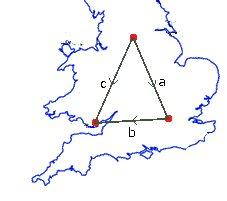
\includegraphics[scale=0.3]{uk}
     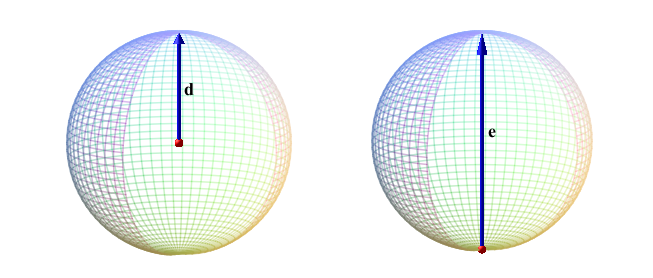
\includegraphics[scale=0.2]{globes}
    \end{center}
   } \uncover<5->{
    Once we have agreed on where our axes should point, and
    what units of length we should use, we can identify $U$
    with $\R^3$. 
   } 
  \end{example}
 }
\end{frame}

% 
\begin{frame}[t]
 \frametitle{The space of functions}
 \uncover<2->{
  \begin{example}{eg-FR}
   The set $F(\R)$ of all functions from $\R$ to $\R$ is a
   vector space, because we can add any two functions to get a
   new function, and we can multiply a function by a number to
   get a new function.
   \vspace{3ex}
   
   \uncover<3->{For example, we can define functions
    $f,g,h\:\R\xra{}\R$ by
    \[
     f(x) = e^x \hspace{4em}
     g(x) = e^{-x} \hspace{4em}
     h(x) = \cosh(x) = \frac{e^x + e^{-x}}{2},
    \]
    so $f$, $g$ and $h$ are elements of $F(\R)$.  
    \vspace{3ex}
    
   }
   \uncover<4->{Then $f+g$
    and $2h$ are again functions, in other words $f+g\in F(\R)$
    and $2h\in F(\R)$.  Of course we actually have $f+g=2h$ in
    this example.
    \vspace{3ex}
    
   }
   \uncover<5->{
    For this to work properly, we must insist that $f(x)$ is
    defined for all $x$, and is a real number for all $x$; it
    cannot be infinite or imaginary.  Thus the rules $p(x)=1/x$
    and $q(x)=\sqrt{x}$ do not define elements $p,q\in F(\R)$.
   }
  \end{example}
 }
\end{frame}

% 
\begin{frame}[t]
 \frametitle{Smaller spaces of functions}
 \uncover<2->{
  \begin{example}{eg-CR}
   In practise, we do not generally want to consider the set
   $F(\R)$ of \emph{all} functions.  
   \uncover<3->{Instead we consider
    \begin{itemize}
    \item The set $C(\R)$ of continuous functions
     \uncover<4->{
     \item The set $C^\infty(\R)$ of ``smooth'' functions\\ 
      (those which can be differentiated arbitrarily often)
     } \uncover<5->{ 
     \item the set $\R[x]$ of polynomial functions \\
      \uncover<6->{(eg $p(x)=1+x+x^2+x^3$ defines an element $p\in\R[x]$)}
     }
    \end{itemize}}
   \uncover<7->{If $f$ and $g$ are continuous then
    $f+g$ and $tf$ are continuous, so $C(\R)$ is a vector
    space.
    \vspace{2ex}
    
   }  
   \uncover<8->{
    If $f$ and $g$ are smooth then $f+g$ and $tf$ are
    smooth, so $C^\infty(\R)$ is a vector space.  
    \vspace{2ex}
    
   }
   \uncover<9->{
    If $f$ and $g$ are polynomials then $f+g$ and $tf$
    are polynomials, so $\R[x]$ is a vector space.
   }
  \end{example}
 }
\end{frame}

% 
\begin{frame}[t]
 \frametitle{Smaller spaces of functions}
 \uncover<2->{\begin{example}{eg-Cab}
   Let $[a,b]$ denote the interval
   $\{x\in\R\st a\leq x\leq b\}$
   \bigskip
   
   \uncover<3->{We write $C[a,b]$ for
    the set of continuous functions $f\:[a,b]\xra{}\R$.
    \bigskip
    
   }
   \uncover<4->{
    For example, the rule $f(x)=1/x$ defines a continuous function
    on the interval $[1,2]$.
   }
   \uncover<5->{  
    (The only potential problem is at the point $x=0$, but
    $0\not\in[1,2]$, so we do not need to worry about it.)
    \bigskip
    
   }
   \uncover<6->{
    We thus have an element $f\in C[1,2]$. 
    \bigskip
    
   }
   \uncover<7->{
    We can define another element $g\in C[1,2]$ by
    $g(x)=2/|x|$.
    \bigskip
    
   }
   \uncover<8->{
    We actually have $g=2f$, because $f$ and $g$ are defined as
    functions on $[1,2]$, and $|x|=x$ for all $x\in[1,2]$.
   }
  \end{example}}
\end{frame}

% 
\begin{frame}[t]
 \frametitle{Spaces of matrices}
 \uncover<2->{\begin{example}{eg-matrices}
   The set $M_2\R$ of $2\tm 2$ matrices (with real entries) is
   a vector space. \uncover<3->{
    Indeed, if we add two such matrices, we
    get another $2\tm 2$ matrix, for example
    \[ \bsm 1 & 0 \\ 0 & 4 \esm + \bsm 0 & 2 \\ 3 & 0 \esm =
     \bsm 1 & 2 \\ 3 & 4 \esm.
    \]
   }
   \uncover<4->{
    Similarly, if we multiply a $2\tm 2$ matrix by a real
    number, we get another $2\tm 2$ matrix, for example
    \[ 7 \bsm 1 & 2 \\ 3 & 4 \esm = \bsm 7 & 14 \\ 21 & 28 \esm. \]
   }
   \uncover<5->{
    We can identify $M_2\R$ with $\R^4$, by the rule
    \[ \bsm a & b \\ c & d \esm \leftrightarrow
     \bsm a \\ b \\ c \\ d \esm.
    \]
   }
   \uncover<6->{
    More generally, for any $n$ the set $M_n\R$ of $n\tm n$
    square matrices is a vector space, which can be identified
    with $\R^{n^2}$.  \bigskip\par
   }
   \uncover<7->{
    More generally still, for any $n$ and
    $m$, the set $M_{n,m}\R$ of $n\tm m$ matrices is a vector
    space, which can be identified with $\R^{nm}$.
   }
  \end{example}}
\end{frame}

\begin{frame}[t]
 \frametitle{The set of all lists}
 \uncover<2->{\begin{example}{eg-lists}
   Let $L$ be the set of all finite lists of real numbers.
   \medskip
   
   For example, the lists $\va=(10,20,30,40)$ and
   $\vb=(5,6,7)$ and $\vc=(1,\pi,\pi^2)$ define three elements
   $\va,\vb,\vc\in L$.  
   \uncover<3->{
    Is $L$ a vector space?  
    \medskip
    
   }
   \uncover<4->{
    In trying to
    answer this question, we will reveal some inadequacies of
    Predefinition~\ref{predef-vector-space}. 
    \medskip
    
   }
   \uncover<5->{
    It seems clear that $L$ is closed under scalar
    multiplication: for example $100\vb=(500,600,700)$, which
    is another element of $L$.
    \medskip
    
   }
   \uncover<6->{
    
    The real issue is closure under
    addition.  \\
    For example, is $\va+\vb$ an element of $L$?  
    \medskip
    
   }
   
   \uncover<7->{
    We cannot answer this unless we know what $\va+\vb$ means.
   }
  \end{example}
 }
\end{frame}

\begin{frame}[t]
 \frametitle{The set of all lists}
 \uncover<2->{
  \[ L = \{\text{ all finite lists of real numbers }\}
   \hspace{2em}
   \va=(10,20,30,40) 
   \hspace{2em}
   \vb=(5,6,7)
  \]
  \medskip
  What does $\va+\vb$ mean?
 }
 \uncover<3->{There are at least three possible meanings:}
 \uncover<4->{
  \begin{itemize}
  \item[(1)] $\va+\vb$ could mean $(10,20,30,40,5,6,7)$ \\
   (the list $\va$ followed by the list $\vb$).
   \uncover<5->{\item[(2)] $\va+\vb$ could mean $(15,26,37)$\\
    (chop off $\va$ to make the lists the same length, then
    add them together).}
   \uncover<6->{\item[(3)] $\va+\vb$ could mean $(15,26,37,40)$\\ 
    (add zeros to the end of $\vb$ to make the lists the same
    length, then add them together.)}
  \end{itemize}
 }
 \uncover<7->{
  The point is that the expression $\va+\vb$ does not have a
  meaning until we decide to give it one.
  \medskip
  
 }  
 \uncover<8->{(Strictly
  speaking, the same is true of the expression $100\vb$, but
  in that case there is only one reasonable possibility for
  what it should mean.)
  \medskip 
  
 }   
\end{frame}

\begin{frame}[t]
 \frametitle{The set of all lists}
 \uncover<2->{
  To avoid this kind of ambiguity, we
  should say that a vector space is a set \emph{together with
   a definition of addition} etc.
  \medskip
  
 }
 \uncover<3->{
  Suppose we use the 3rd definition of addition,
  so $\va+\vb=(15,26,37,40)$.  
  \medskip
  
 }
 \uncover<4->{
  The ordinary rules of
  algebra would tell us that $(\va + (-1).\va) + \vb=\vb$.
  \medskip
  
 }
 \uncover<5->{ 
  However, in fact we have
  \begin{align*}
   (\va + (-1).\va) + \vb &=
   ((10,20,30,40) + (-10,-20,-30,-40)) + (5,6,7) \\
   &= (0,0,0,0) + (5,6,7) = (5,6,7,0) 
   \RED{\neq} (5,6,7) = \vb. \vspace{-3ex}
  \end{align*}
  Thus, the ordinary rules of algebra do not hold.  
  \medskip
  
 }
 \uncover<6->{
  We do not want to deal with this kind of thing; we only want to
  consider sets where addition and scalar multiplication work
  in the usual way.  We must therefore give a more careful
  definition of a vector space, which will allow us to say
  that $L$ is not a vector space, so we need not think about
  it. 
  \medskip
  
 }
 \uncover<7->{
  (If we used either of the other definitions of addition
  then things would still go wrong; details are left as an
  exercise.)
  
 }
\end{frame}

\begin{frame}[t]
 \frametitle{A more precise definition}
 \uncover<2->{
  Our next attempt at a definition is as follows:
  \bigskip
  
 }
 \uncover<3->{
  \begin{predefinition}{predef-vector-space-ii}
   A \DEFN{vector space} over $\R$ is a nonempty set $V$, together
   with a definition of what it means to add elements of $V$
   or multiply them by real numbers, such that
   \begin{itemize}
   \item[(a)] If $u$ and $v$ are elements of $V$, then $u+v$ is an
    also an element of $V$.
   \item[(b)] If $u$ is an element of $V$ and $t$ is a real number, then
    $tu$ is an element of $V$.
   \item[(c)] All the usual algebraic rules for addition and
    multiplication hold.
   \end{itemize}
  \end{predefinition}
  \bigskip
  
 }
 \uncover<4->{
  In the course we will be content with an informal
  understanding of the phrase ``all the usual algebraic
  rules'', but for completeness, we will give an explicit list of
  axioms.
 }
\end{frame}

\begin{frame}[t]
 \frametitle{The real definition}
 \uncover<2->{
  \begin{definition}{defn-real-vector-space}
   A \DEFN{vector space} over $\R$ is a set $V$, together with an
   element $0\in V$ and a definition of what it means to add
   elements of $V$ or multiply them by real numbers%
   \uncover<3->{, such that
    \begin{itemize} 
    \item[(a)] If $u$ and $v$ are elements of $V$, then $u+v$
     is an also an element of $V$.
    \item[(b)] If $v$ is an element of $V$ and $t$ is a real
     number, then $tv$ is an element of $V$.
     \uncover<4->{
     \item[(c)] For any elements $u,v,w\in V$ and any real
      numbers $s,t$, the following equations hold:\\
      \parbox{6cm}{\begin{itemize}
       \item[(1)] $0+v=v$
       \item[(2)] $u+v=v+u$
       \item[(3)] $u+(v+w)=(u+v)+w$
       \item[(4)] $0u=0$
       \end{itemize}}
      \parbox{4cm}{\begin{itemize}
       \item[(5)] $1u=u$
       \item[(6)] $(st)u=s(tu)$
       \item[(7)] $(s+t)u=su+tu$
       \item[(8)] $s(u+v)=su+sv$.
       \end{itemize}}
     }
    \end{itemize} 
   } 
  \end{definition}
  \uncover<5->{
   Note that there are many rules that do not appear explicitly
   in the above list, such as the fact that
   $t(u+v-w/t)=tu+tv-w$, but it turns out that all such rules
   can be deduced from the ones listed.  We will not discuss
   any such deductions.
  }}
\end{frame}

\begin{frame}[t]
 \frametitle{Zero}
 \uncover<2->{
  \begin{remark}{rem-zero-notation}
   We will usually use the symbol $0$ for the zero element of
   whatever vector space we are considering.  
   \bigskip
   
   \uncover<3->{
    Thus $0$ could mean 
    \begin{itemize}
    \item the vector $\bsm 0\\0\\0\esm$ 
     \hspace{6.06em} (if we are working with $\R^3$)
     \uncover<4->{
     \item the zero matrix $\bsm 0&0&0\\0&0&0\esm$
      \hspace{2.9em} (if we are working with $M_{2,3}\R$)}
     \uncover<5->{
     \item the zero function 
      \hspace{5em} (if we are working with $C(\R)$)}
    \end{itemize}
   }
   \uncover<6->{or whatever.
    \bigskip
    
   }
   \uncover<7->{
    Occasionally it will be important to distinguish between
    the zero elements in different vector spaces.  In that
    case, we write $0_V$ for the zero element of $V$.  
    \bigskip
    
   }
   \uncover<8->{
    For example:
    \[ 0_{\R^2}=\bsm 0\\0\esm \hspace{4em}
     0_{M_2\R}=\bsm 0&0\\0&0\esm.
    \]
   }
  \end{remark}
 }
\end{frame}

\begin{frame}[t]
 \frametitle{Vector spaces over other fields}
 \uncover<2->{
  One can also consider vector spaces over fields other than
  $\R$; the most important case for us will be the field $\C$
  of complex numbers.  We record the definitions for
  completeness. 
  \bigskip
  
 }
 \uncover<3->{
  \begin{definition}{defn-field}
   A \DEFN{field} is a set $K$ together with elements
   $0,1\in K$ and a definition of what it means to add or
   multiply two elements of $K$\uncover<4->{, such that:
    \begin{enumerate}
    \item[(a)] The usual rules of algebra are valid.  
     \uncover<5->{
      More explicitly, for all $a,b,c\in K$ the following equations hold: \\
      \parbox{6cm}{
       \begin{itemize}
       \item $0+a=a$
       \item $a+(b+c)=(a+b)+c$
       \item $a+b=b+a$
       \item $1.a=a$
       \end{itemize}}
      \parbox{4cm}{
       \begin{itemize}
       \item $a(bc)=(ab)c$
       \item $ab=ba$
       \item $a(b+c)=ab+ac$
       \end{itemize}}
     }
     \uncover<6->{
     \item[(b)] For every $a\in K$ there is an element $-a$ with
      $a+(-a)=0$.}
     \uncover<7->{
     \item[(c)] For every $a\in K$ with $a\neq 0$ there is an
      element $a^{-1}\in K$ with $aa^{-1}=1$.}
     \uncover<8->{
     \item[(d)] $1\neq 0$ \hspace{2em}
      (or equivalently, $K\neq\{0\}$).}
    \end{enumerate}}
  \end{definition}
 }
\end{frame}

\begin{frame}[t]
 \frametitle{Examples of fields}
 \uncover<2->{
  \begin{example}{eg-fields}
   Recall that 
   \begin{align*}
    \Z &= \{ \text{ integers } \} =
    \{ \dotsc,-2,-1,0,1,2,3,4,\dotsc \} \\
    \Q &= \{ \text{ rational numbers } \} =
    \{ a/b\st a,b\in\Z\;,\; b\neq 0\} \\
    \R &= \{ \text{ real numbers } \} \\
    \C &= \{ \text{ complex numbers } \} = 
    \{ x+iy\st x,y\in\R \},
   \end{align*}
   \uncover<3->{so $\Z\subset\Q\subset\R\subset\C$.
    \bigskip
    
   }  
   \uncover<4->{
    Then $\R$, $\C$ and $\Q$ are fields.
    \bigskip
    
   }  
   \uncover<5->{
    The ring $\Z$ is not a field, because axiom~(c) is not
    satisfied: there is no element $2^{-1}$ \emph{in the
     set $\Z$} for which $2.2^{-1}=1$.
    \bigskip
    
   }  
   \uncover<6->{
    One can show that the ring $\Z/n\Z$ is a field if and only
    if $n$ is a prime number.
   }
  \end{example}
 }
\end{frame}

\begin{frame}[t]
 \frametitle{Vector spaces over other fields}
 \uncover<2->{
  \begin{definition}{defn-vector-space}
   A \DEFN{vector space} over a field $K$ is a set $V$, together with
   an element $0\in V$ and a definition of what it means to
   add elements of $V$ or multiply them by elements of $K$
   \uncover<3->{, such that
    \begin{itemize}
    \item[(a)] If $u$ and $v$ are elements of $V$, then $u+v$ is an
     also an element of $V$.
    \item[(b)] If $v$ is an element of $V$ and $t$ is an
     element of $K$, then $tv\in V$.
     \uncover<4->{\item[(c)] For any elements $u,v,w\in V$ and any elements
      $s,t\in K$, the following equations hold:\\
      \parbox{6cm}{\begin{itemize}
       \item[(1)] $0+v=v$
       \item[(2)] $u+v=v+u$
       \item[(3)] $u+(v+w)=(u+v)+w$
       \item[(4)] $0u=0$
       \end{itemize}}
      \parbox{4cm}{\begin{itemize}
       \item[(5)] $1u=u$
       \item[(6)] $(st)u=s(tu)$
       \item[(7)] $(s+t)u=su+tu$
       \item[(8)] $s(u+v)=su+sv$.
       \end{itemize}}
     }
    \end{itemize}  
   }
  \end{definition}
 }
 \uncover<5->{\begin{example}{eg-other-fields}
   Almost all our examples work over any field $K$.\\  
   \uncover<6->{$M_4\Q=\{4\tm 4 \text{ matrices with entries
     in } \Q\}$ is a vector space over $\Q$.\\}
   \uncover<7->{$\C[x]=\{\text{polynomials with
     complex coefficients}\}$ is a vector space over $\C$.
   }
  \end{example}}
 
\end{frame}

\begin{frame}[t]
 \frametitle{Linear maps}
 \uncover<2->{
  \begin{definition}{defn-linear}
   Let $V,W$ be vector spaces.  Let $\phi\:V\xra{}W$ be a
   function \\
   \uncover<3->{
    (so for each element $v\in V$ we have an element
    $\phi(v)\in W$).\\}
   \uncover<4->{
    We say that $\phi$ is \DEFN{linear} if 
    \begin{itemize}
     \uncover<5->{\item[(a)] For any $v$ and $v'$ in $V$, we have
      $\phi(v+v')=\phi(v)+\phi(v')$ in $W$.}
     \uncover<6->{\item[(b)] For any $t\in\R$ and $v\in V$ we have
      $\phi(tv)=t\phi(v)$ in $W$. }
    \end{itemize}
   }
   \uncover<7->{By taking $t=v=0$ in~(b), we see that a linear map must satisfy
    $\phi(0)=0$.
    \bigskip
    
   }
   \uncover<8->{
    Further simple arguments also show that
    $\phi(v-v')=\phi(v)-\phi(v')$.
   }
  \end{definition}
  \bigskip
  
 }
 \uncover<9->{\begin{remark}{rem-linear-condensed}
   The definition can be reformulated slightly as follows.  A
   map $\phi\:V\to W$ is linear iff
   \begin{itemize}
   \item[(c)] For any $t,t'\in\R$ and any $v,v'\in V$ we have
    $\phi(tv+t'v')=t\phi(v)+t'\phi(v')$. 
   \end{itemize}
   \uncover<10->{
    To show that this reformulation is valid, we must show that
    if~(c) holds, then so do~(a) and~(b); and conversely,
    if~(a) and~(b) hold, then so does~(c).
    \bigskip
    
   }
   \uncover<11->{This is left as an exercise.}
  \end{remark}
 }
\end{frame}

\begin{frame}[t]
 \frametitle{Linear maps}
 \uncover<2->{
  \begin{definition}{defn-linear}
   Let $V,W$ be vector spaces.  Let $\phi\:V\xra{}W$ be a
   function \\
   \uncover<3->{
    (so for each element $v\in V$ we have an element
    $\phi(v)\in W$).\\}
   \uncover<4->{
    We say that $\phi$ is \DEFN{linear} if 
    \begin{itemize}
     \uncover<5->{\item[(a)] For any $v$ and $v'$ in $V$, we have
      $\phi(v+v')=\phi(v)+\phi(v')$ in $W$.}
     \uncover<6->{\item[(b)] For any $t\in\R$ and $v\in V$ we have
      $\phi(tv)=t\phi(v)$ in $W$. }
    \end{itemize}
   }
   \uncover<7->{By taking $t=v=0$ in~(b), we see that a linear map must satisfy
    $\phi(0)=0$.
    \bigskip
    
   }
   \uncover<8->{
    Further simple arguments also show that
    $\phi(v-v')=\phi(v)-\phi(v')$. 
   }
  \end{definition}
  \bigskip
  
 }
 \uncover<9->{\begin{remark}{rem-linear-condensed}
   The definition can be reformulated slightly as follows.  A
   map $\phi\:V\to W$ is linear iff
   \begin{itemize}
   \item[(c)] For any $t,t'\in\R$ and any $v,v'\in V$ we have
    $\phi(tv+t'v')=t\phi(v)+t'\phi(v')$. 
   \end{itemize}
   \uncover<10->{
    To show that this reformulation is valid, we must show that
    if~(c) holds, then so do~(a) and~(b); and conversely,
    if~(a) and~(b) hold, then so does~(c).
    \bigskip
    
   }
   \uncover<11->{This is left as an exercise. \;\es}
  \end{remark}
 }
\end{frame}

\begin{frame}[t]
 \frametitle{Linear maps from $\R$ to $\R$}
 \uncover<2->{\begin{example}{eg-square-nonlinear}
   Consider $f,g\:\R\xra{}\R$ given by $f(x)=2x$ and
   $g(x)=x^2$.\bigskip\par
   \uncover<3->{
    $g(x+x') = x^2 + x'^2 + 2xx' \neq x^2 + x'^2 = g(x) + g(x'),$
    so $g$ is not linear.  \bigskip\par
    
   }
   \uncover<4->{
    Similarly, $\sin(x+x')\neq\sin(x)+\sin(x')$ so $\sin$
    is not linear.  
   }  \uncover<5->{  
    \begin{align*}
     \hspace{-2em} \text{ On the other hand: } \hspace{3em} f(x+x') &=
     2(x+x') = 2x + 2x' = f(x) + f(x') \\
     f(tx) &= 2tx = t f(x)  \hspace{3em}\text{ so $f$ is linear. }
    \end{align*}
   }
  \end{example}}
 
 \uncover<6->{\begin{example}{eg-LRR}
   For any number $m\in\R$, we can define
   $\mu_m\:\R\xra{}\R$ by $\mu_m(x)=mx$ 
   \uncover<7->{(so $f$ in the
    previous example is $\mu_2$).}  
   \uncover<8->{We have
    \begin{align*}
     \mu_m(x+x') &= m(x+x') = mx+mx' = \mu_m(x) + \mu_m(x') \\
     \mu_m(tx)   &= mtx = tmx = t\mu_m(x),
    \end{align*}}
   \uncover<9->{so $\mu_m$ is linear.}
   \uncover<10->{Note also that the graph of
    $\mu_m$ is a straight line of slope $m$ through the origin;
    this is essentially the reason for the word ``linear''. \quad\es}
  \end{example}
 }
\end{frame}

\begin{frame}[t]
 \frametitle{Rotation is linear}
 \uncover<2->{
  \begin{example}{eg-rot-linear}
   For any $\vv\in\R^2$, we let $\rho(\vv)$ be the vector obtained
   by rotating $\vv$ through $90$ degrees anticlockwise around
   the origin.
   \uncover<3->{
    It is well-known that the formula for this is
    $\rho\bsm x\\ y\esm=\bsm -y\\ x\esm$.
    \begin{center}
     \begin{tikzpicture}[scale=2]
      \draw[->] (-0.7,0) -- (1.2,0);
      \draw[->] (0,-0.2) -- (0,1.2);
      \draw[blue] (0,0) -- ( 0.8, 0.6);
      \draw[blue] (0,0) -- (-0.6, 0.8);
      \draw[dotted] ( 0.8, 0.6) -- ( 0.8, 0.0);
      \draw[dotted] (-0.6, 0.8) -- ( 0.0, 0.8);
      \draw( 1.00, 0.6) node {$\bsm x \\ y\esm$};
      \draw(-0.85, 0.8) node {$\bsm -y \\ x\esm$};
      \fill ( 0.0, 0.0) circle(0.03);
      \fill ( 0.8, 0.6) circle(0.03);
      \fill (-0.6, 0.8) circle(0.03);
     \end{tikzpicture}
    \end{center}}
   \uncover<4->{We thus have
    \begin{align*}
     \rho\left(\bsm \xx\\\yy\esm+\bsm x'\\ y'\esm\right) &=
     \rho\bsm \xx+x'\\ \yy+y'\esm =
     \bsm -\yy-y'\\ \xx+x'\esm =
     \bsm -\yy\\ \xx\esm + \bsm -y'\\ x'\esm = 
     \rho\bsm \xx\\ \yy\esm + \rho\bsm x'\\ y'\esm \\
     \rho\left(t\bsm \xx\\ \yy\esm\right) &=
     \rho\bsm t\xx\\ t\yy\esm =
     \bsm -t\yy \\ t\xx\esm = 
     t\rho\bsm \xx\\ \yy\esm,
    \end{align*}
    so $\rho$ is linear. \quad\es}
  \end{example}}
\end{frame}

\begin{frame}[t]
 \frametitle{More general rotations}
 \uncover<2->{More generally, let $\text{rot}_\theta(\vv)$ be the vector
  obtained by rotating $\vv$ anticlockwise by an angle of
  $\tht$ around the origin.}
 \bs
 \uncover<3->{Then
  \[ \text{rot}_\theta\bsm x\\ y\esm =
   \bsm \cos(\theta)x - \sin(\theta)y \\
   \sin(\theta)x + \cos(\theta)y \esm
  \]}\bs
 \uncover<4->{Using this, we see that $\text{rot}_\theta\:\R^2\to\R^2$ is
  a linear map. \quad\es}
\end{frame}

\begin{frame}[t]
 \frametitle{Reflection is linear}
 \uncover<2->{\begin{example}{eg-ref-linear}
   For any $\vv\in\R^2$, we let $\tau(\vv)$ be the vector
   obtained by reflecting $\vv$ across the line $y=0$.
   \bigskip
   
   \uncover<3->{It is
    clear that the formula is
    $\tau\bsm x\\ y\esm=\bsm x\\-y\esm$, and using this we see
    that $\tau$ is linear.
    \begin{center}
     \begin{tikzpicture}[scale=2]
      \draw[->] (-0.5,0) -- (1.5,0);
      \draw[->] (0,-0.8) -- (0,0.8);
      \draw (0,0) -- (0.8,0.6);
      \draw (0,0) -- (0.8,-0.6);
      \draw[dotted] ( 0.8,0.6) -- (0.8,-0.6);
      \draw (1, 0.6) node{$\bsm x \\  y\esm$};
      \draw (1,-0.6) node{$\bsm x \\ -y\esm$};
      \fill (0,0) circle(0.03);
      \fill (0.8,0.6) circle(0.03);
      \fill (0.8,-0.6) circle(0.03);
     \end{tikzpicture}
    \end{center}
    \es}
  \end{example}}
\end{frame}

\begin{frame}[t]
 \frametitle{More general reflections}
 \uncover<2->{More generally, let $\text{ref}_\theta(\vv)$ be the vector
  obtained by reflecting $\vv$ across the line crossing the
  $x$-axis at an angle of $\theta/2$.}
 \bs
 \uncover<3->{Then
  \[ \text{ref}_\theta\bsm x\\ y\esm =
   \bsm \cos(\theta)x + \sin(\theta)y \\
   \sin(\theta)x - \cos(\theta)y \esm
  \]}\bs
 \uncover<4->{Using this, we see that $\text{ref}_\theta\:\R^2\to\R^2$ is
  a linear map.  \quad\es}
\end{frame}

\begin{frame}[t]
 \frametitle{Some nonlinear examples}
 \uncover<2->{\begin{example}{eg-norm-nonlinear}
   Define $\tht\:\R^2\xra{}\R$ by $\tht(\vv)=\|\vv\|$
   \uncover<3->{ so $\tht\bsm x\\ y\esm=\sqrt{x^2+y^2}$.\\}
   \uncover<4->{ This is not linear,
    because $\tht(\vu+\vv)\neq\tht(\vu)+\tht(\vv)$ in
    general.\\}
   \uncover<5->{
    Indeed, if $\vu=\bsm 1\\0\esm$ and $\vv=\bsm -1\\0\esm$
    then $\tht(\vu+\vv)=0$ but $\tht(\vu)+\tht(\vv)=1+1=2$.}
  \end{example}
  \bigskip
  
 }
 \uncover<6->{
  \begin{example}{eg-shift-nonlinear}
   Define $\sg\:\R^2\xra{}\R^2$ by
   $\sg\bsm x\\ y\esm=\bsm x+1\\ y-1\esm$.  \\
   \uncover<7->{Then
    $\sg$ is not linear, because
    $\sg\bsm 0\\0\esm\neq\bsm 0\\0\esm$.}
  \end{example}\bigskip\par}
 \uncover<8->{\begin{example}{eg-homogeneous-nonlinear}
   Define $\al\:\R^2\to\R^2$ by 
   $\displaystyle \al\bsm x \\ y\esm =
   \bsm y^3/(x^2+y^2) \\ x^3/(x^2+y^2) \esm.
   $\\
   \uncover<9->{(This does not really make sense when
    $x=y=0$, but for that case we make the separate definition
    that $\al\bsm 0\\0\esm=\bsm 0\\0\esm$.)\\}
   \uncover<10->{This map satisfies
    $\al(t\vv)=t\al(\vv)$, but it does not satisfy
    $\al(\vu+\vv)=\al(\vu)+\al(\vv)$, so it is not linear.
    \bigskip\par
   }
   \uncover<11->{
    For example, if $\vu=\bsm 1\\0\esm$ and $\vv=\bsm 0\\1\esm$
    then $\al(\vu)=\vv$ and $\al(\vv)=\vu$ but
    $\al(\vu+\vv)=(\vu+\vv)/2\neq\al(\vu)+\al(\vv)$. \quad\es}
  \end{example}}
 
\end{frame}

\begin{frame}[t]
 \frametitle{Examples from vector algebra}
 \uncover<2->{\begin{example}{eg-vector-algebra}
   Given vectors $\vu=\bsm u_1\\ u_2\\ u_3\esm$ and
   $\vv=\bsm v_1\\ v_2\\ v_3\esm$ in $\R^3$, recall that the
   inner product and cross product are defined by 
   \begin{align*}
    \ip{\vu,\vv} &= \vu . \vv = u_1v_1 + u_2v_2 + u_3v_3 \\
    \vu\tm\vv &= \bsm u_2 v_3 - u_3 v_2 \\
    u_3 v_1 - u_1 v_3 \\
    u_1 v_2 - u_2 v_1 \esm.
   \end{align*}
\ifx\HO\undefined
   \only<3>{
    \[ \det\bsm \ve_1&\ve_2&\ve_3 \\
     u_1 & u_2 & u_3 \\
     v_1 & v_2 & v_3 \esm = 
     \det\bsm u_2 & u_3 \\ v_2 & v_3 \esm \ve_1 - 
     \det\bsm u_1 & u_3 \\ v_1 & v_3 \esm \ve_2 + 
     \det\bsm u_1 & u_2 \\ v_1 & v_2 \esm \ve_3 =
     \bsm u_2 v_3 - u_3 v_2 \\
     u_3 v_1 - u_1 v_3 \\
     u_1 v_2 - u_2 v_1 \esm =
     \vu \tm \vv 
    \]
   }
\fi
   \uncover<4->{Fix a vector $\va\in\R^3$.  Define $\al\:\R^3\xra{}\R$ by
    $\al(\vv)=\ip{\va,\vv}$ and $\bt\:\R^3\xra{}\R^3$ by
    $\bt(\vv)=\va\tm\vv$.  Then both $\al$ and $\bt$ are
    linear. \medskip\par}%
   \uncover<5->{To prove this we must show that
    $\al(t\vv)=t\al(\vv)$ and $\al(\vv+\vw)=\al(\vv)+\al(\vw)$
    and $\bt(t\vv)=t\bt(\vv)$ and
    $\bt(\vv+\vw)=\bt(\vv)+\bt(\vw)$.\\
   }%
   \uncover<6->{We will write out only
    the last of these; the others are similar but easier.
    \begin{align*} 
     \uncover<7->{\bt(\vv+\vw) = 
      \bt\bsm v_1+w_1 \\ v_2+w_2 \\ v_3+w_3 \esm} &
     \uncover<8->{= 
      \bsm a_2(v_3+w_3) - a_3(v_2+w_2) \\
      a_3(v_1+w_1) - a_1(v_3+w_3) \\
      a_1(v_2+w_2) - a_2(v_1+w_1) \esm
      \hspace{10em}{\WHITE{.}}} \\ &
     \uncover<9->{= 
      \bsm a_2 v_3 - a_3 v_2 \\
      a_3 v_1 - a_1 v_3 \\
      a_1 v_2 - a_2 v_1 \esm +
      \bsm a_2 w_3 - a_3 w_2 \\
      a_3 w_1 - a_1 w_3 \\
      a_1 w_2 - a_2 w_1 \esm}
     \uncover<10->{= \bt(\vv) + \bt(\vw).  \quad\es}
    \end{align*}
   }\end{example}}
\end{frame}

\begin{frame}[t]
 \frametitle{Multiplication by a matrix is linear}
 \uncover<2->{
  \begin{example}{eg-matrix-linear}
   Let $A$ be a fixed $m\tm n$ matrix.  \medskip\par
   \uncover<3->{Given a vector $\vv\in\R^n$, we can multiply $A$ by
    $\vv$ to get a vector $A\vv\in\R^m$.  \medskip\par}
   \uncover<4->{We can thus define $\phi_A\:\R^n\xra{}\R^m$ by
    $\phi_A(\vv)=A\vv$. \medskip\par} 
   \uncover<5->{It is clear that
    $A(\vv+\vv')=A\vv+A\vv'$ and $At\vv=tA\vv$, so $\phi_A$ is
    a linear map. \medskip\par}  
   \uncover<6->{We will see later that every linear map from
    $\R^n$ to $\R^m$ has this form.
    \medskip\par
   }
   \uncover<7->{
    In particular, if we put
    $R = \bsm 0 & -1 \\ 1 & 0 \esm$ and 
    $T = \bsm 1 & 0 \\ 0 & -1 \esm$}\uncover<8->{, we find that 
    \[ 
     R\bsm x \\ y\esm = \bsm -y\\ x\esm = 
     \rho\left(\bsm x\\ y\esm\right) \hspace{5em}
     T\bsm x \\ y\esm = \bsm x\\ -y\esm = 
     \tau\left(\bsm x\\ y\esm\right)
    \]
    (where $\rho$ and $\tau$ are as in
    Examples~\ref{eg-rot-linear} and~\ref{eg-ref-linear}).\\}
   \uncover<9->{This means that $\rho=\phi_R$ and
    $\tau=\phi_T$.\bs}
   \uncover<10->{More generally, $\text{rot}_\theta=\phi_{R_\theta}$
    and $\text{ref}_\theta=\phi_{T_\theta}$, where 
    \[ R_\theta = \bsm \cos(\theta) & -\sin(\theta) \\
     \sin(\theta) & \cos(\theta) \esm
     \hspace{3em}
     T_\theta = \bsm \cos(\theta) & \sin(\theta) \\
     \sin(\theta) & -\cos(\theta) \esm  \quad\es
    \]}
  \end{example}
 }
\end{frame}

\begin{frame}[t]
 \frametitle{Definite integration is linear}
 \uncover<2->{
  \begin{example}{eg-int-linear}
   For any continuous function $f\:\R\xra{}\R$, we write
   \[ I(f) = \textstyle\int_0^1f(x)dx \in \R. \]
   \uncover<3->{This defines a map $I\:C(\R)\xra{}\R$.\\}
   \uncover<4->{\vspace{-2ex}
    \begin{align*}
     p(x) &= x^2   & 
     \uncover<5->{I(p)} & \uncover<5->{= \textstyle\int_0^1 x^2\,dx}
     \uncover<6->{ = [x^3/3]_0^1}\uncover<7->{ = 1/3 \hspace{5em}\WHITE{.}} \\
     \uncover<8->{q(x)} &\uncover<8->{= 2x-1}  & 
     \uncover<9->{I(q)} & \uncover<9->{= \textstyle\int_0^1 2x-1\,dx}
     \uncover<10->{= [x^2-x]_0^1} \uncover<11->{ = 0} \\
     \uncover<12->{r(x)} &\uncover<12->{= e^x}   & 
     \uncover<13->{I(r)} &\uncover<13->{= \textstyle\int_0^1 e^x\,dx}
     \uncover<14->{ = [e^x]_0^1} \uncover<15->{ = e-1.}
    \end{align*}}
   \uncover<16->{
    Using the obvious equations
    \begin{align*}
     \textstyle\int_0^1 f(x)+g(x) dx &=
     \textstyle\int_0^1 f(x)dx + \textstyle\int_0^1 g(x) dx \\
     \textstyle\int_0^1 t f(x) dx &= t \textstyle\int_0^1 f(x) dx 
    \end{align*}
    we see that $I(f+g)=I(f)+I(g)$ and $I(tf)=t\,I(f)$, so $I$
    is a linear map.\es
   }
  \end{example}
 }
\end{frame}

\begin{frame}[t]
 \frametitle{Linear differential operators}
 \uncover<2->{
  \begin{definition}{eg-diff-linear}
   For smooth $f\:\R\xra{}\R$ put $D(f)=f'$ and
   $L(f)=f''+f$.  \bigskip\par
   \uncover<3->{These are again smooth, so 
    $D\:C^\infty(\R)\xra{}C^\infty(\R)$ and
    $L\:C^\infty(\R)\xra{}C^\infty(\R)$. }
   \uncover<4->{\begin{align*}
     \uncover<4->{p(x)} &\uncover<4->{=\sin(x)} & \uncover<5->{D(p)} &\uncover<5->{= q} &
     \uncover<6->{L(p)} &\uncover<6->{= 0} \\
     \uncover<4->{q(x)} &\uncover<4->{=\cos(x)} & \uncover<5->{D(q)} &\uncover<5->{=-p} &
     \uncover<6->{L(q)} &\uncover<6->{= 0} \\
     \uncover<4->{r(x)} &\uncover<4->{=e^x}     & \uncover<5->{D(r)} &\uncover<5->{= r} &
     \uncover<6->{L(r)} &\uncover<6->{= 2r}
    \end{align*}}
   \uncover<7->{Using the equations
    $(f+g)'=f'+g'$ and $(tf)'=t\;f'$
    we see that $D$ is linear.}  
   \uncover<8->{Similarly, we have
    \begin{align*}
     L(f+g) &= (f+g)'' + (f+g) 
     = f'' + g'' + f + g \\
     &= (f''+f) + (g''+g) 
     = L(f) + L(g) \\
     L(tf)  &= (tf)'' + tf 
     = t\; f'' + t f 
     = t L(f).
    \end{align*}
    This shows that $L$ is also linear. \quad\es}
  \end{definition}
 }
\end{frame}

\begin{frame}[t]
 \frametitle{Trace and determinant}
 \uncover<2->{
  \begin{example}{eg-trace-det}
   For any $2\tm 2$ matrix $A=\bsm a & b\\ c & d\esm$, the
   trace and determinant are defined by $\trace(A)=a+d\in\R$
   and $\det(A)=ad-bc\in\R$.  \ms
   \uncover<3->{We thus have two functions
    $\trace,\det\:M_2\R\xra{}\R$.\ms}  
   \uncover<4->{It is easy to see that
    $\trace(A+B)=\trace(A)+\trace(B)$ and
    $\trace(tA)=t\trace(A)$, so $\trace\:M_2\R\xra{}\R$ is a
    linear map.\ms}  
   \uncover<5->{On the other hand, 
    $\det(tA)=t^2\det(A)$ and $\det(A+B)\neq\det(A)+\det(B)$ in
    general, so $\det\:M_2\R\xra{}\R$ is not a linear map.\ms}
   \uncover<6->{For
    a specific counterexample, take \hspace{1em}
    $\displaystyle A = \bsm 1 & 0 \\ 0 & 0 \esm 
    \hspace{1em} \text{ and } \hspace{1em}
    B = \bsm 0 & 0 \\ 0 & 1 \esm
    $\ms}
   \uncover<7->{
    $\det(A)=\det(B)=0$ but $\det(A+B)=1$, so
    $\det(A+B)\neq\det(A)+\det(B)$.  \ms
   }
   \uncover<8->{None of this is really restricted to $2\tm 2$ matrices.
    For any $n$ we have a map $\trace\:M_n\R\xra{}\R$ given by
    $\trace(A)=\sum_{i=1}^nA_{ii}$, which is again linear.  We
    also have a determinant map $\det\:M_n\R\xra{}\R$ which
    satisfies $\det(tI)=t^n$; this shows that $\det$ is not
    linear, except in the silly case where $n=1$. \quad\es}
  \end{example}
 }
\end{frame}

\begin{frame}[t]
 \frametitle{Matrix inversion is not linear}
 \uncover<2->{
  \begin{example}{eg-inv-nonlinear}
   ``Define'' $\phi\:M_2\R\xra{}M_2\R$ by $\phi(A)=A^{-1}$\uncover<3->{, so
    \[ \phi\bsm a & b \\ c & d\esm =
     \bsm d/(ad-bc) & -b/(ad-bc) \\ -c/(ad-bc) & a/(ad-bc) \esm. 
    \]}
   \uncover<4->{This is not a linear map, simply because it is not a
    well-defined map at all: the ``definition'' does not make
    sense when $ad-bc=0$.\ms}
   \uncover<5->{Even if it were well-defined, it
    would not be linear}\uncover<6->{, because
    $\phi(I+I)=(2I)^{-1}=I/2$}
   \uncover<7->{, whereas $\phi(I)+\phi(I)=2I$}\uncover<8->{, so
    $\phi(I+I)\neq\phi(I)+\phi(I)$. \quad\es}
  \end{example}
 }
\end{frame}

\begin{frame}[t]
 \frametitle{Row reduction is not linear}
 \uncover<2->{
  \begin{example}{eg-rref-nonlinear}
   Define $\phi\:M_3\R\xra{}M_3\R$ by 
   \[ \phi(A)=\text{ the row reduced echelon form of } A. \]
   \uncover<3->{For example, we have the following sequence of reductions:
    \[ \bsm 1&2&3 \\ 4&8&6 \\ 7&14&9 \esm \uncover<4->{\to
      \bsm 1&2&3 \\ 0&0&-6 \\ 0&0&-12 \esm} \uncover<5->{\to
      \bsm 1&2&3 \\ 0&0&1 \\ 0&0&-12 \esm} \uncover<6->{\to
      \bsm 1&2&0 \\ 0&0&1 \\ 0&0&0 \esm}
    \]}
   \uncover<7->{which shows that
    \[ \phi\bsm 1&2&3 \\ 4&8&6 \\ 7&14&9 \esm  = 
     \bsm 1&2&0 \\ 0&0&1 \\ 0&0&0 \esm.
    \]}
   \uncover<8->{The map is not linear, because $\phi(I)=I$ and also
    $\phi(2I)=I$, so $\phi(2I)\neq 2\phi(I)$. \es}
  \end{example}
 }
\end{frame}

\begin{frame}[t]
 \frametitle{Transposition is linear}
 \uncover<2->{
  \begin{example}{eg-transpose-linear}
   We can define a map $\trans\:M_n\R\xra{}M_n\R$ by $\trans(A)=A^T$.\ms
   \uncover<3->{Here as usual, $A^T$ is the transpose of $A$, which is obtained by
    flipping $A$ across the main diagonal.\ms}
   \uncover<4->{For example:
    \[ \bsm 1 & 2 & 3 \\ 0 & 4 & 5 \\ 0 & 0 & 6 \esm^T =
     \bsm 1 & 0 & 0 \\ 2 & 4 & 0 \\ 3 & 5 & 6 \esm.
    \]}
   \uncover<5->{In general, we have $(A^T)_{ij}=A_{ji}$. \ms}
   \uncover<6->{It is clear that 
    $(A+B)^T=A^T+B^T$ and $(tA)^T=tA^T$}\uncover<7->{,\ms
    so $\trans\:M_n\R\xra{}M_n\R$ is a linear map.\bs}
   \uncover<7->{
    e.g. $\left(\bsm a&b\\ c&d\esm + \bsm a'&b'\\ c'&d'\esm\right)^T
    = \bsm a+a'& b+b'\\ c+c'&d+d'\esm^T
    = \bsm a+a'& c+c'\\ b+b'&d+d'\esm
    = \bsm a&b\\ c&d\esm^T + \bsm a'&b'\\ c'&d'\esm^T$\es
   }
  \end{example}
 }
\end{frame}

\begin{frame}[t]
 \frametitle{Isomorphisms}
 \uncover<2->{
  \begin{definition}{defn-iso}\\
   A linear map $\phi\:V\to W$ is an
   \DEFN{isomorphism} if it is a bijection\uncover<3->{,\ms so there is an
    inverse map $\phi^{-1}\:W\xra{}V$ with
    $\phi(\phi^{-1}(w))=w$ for all $w\in W$, and
    $\phi^{-1}(\phi(v))=v$ for all $v\in V$.\ms}
   \uncover<4->{( $\phi^{-1}$ is automatically a \emph{linear}
    map - we leave this as an exercise.) \ms}
   \uncover<5->{Say that $V$ and $W$ are
    \DEFN{isomorphic} if there is an isomorphism from $V$
    to $W$. \ms}
  \end{definition}}
 \uncover<6->{\begin{example}{eg-iso-matrices}
   We can now rephrase part of Example~\ref{eg-matrices} as
   follows:\ms
   \uncover<7->{There is an isomorphism $\phi\:M_2\R\xra{}\R^4$
    given by \[\phi\bsm a&b\\ c&d\esm=\bsm a\\ b\\ c\\ d\esm\]}\uncover<8->{
    so $M_2\R$ is isomorphic to $\R^4$.\ms}
   \uncover<9->{Similarly, the space $M_{p,q}\R$ is
    isomorphic to $\R^{pq}$.\quad\es}
  \end{example}
 }
\end{frame}

\begin{frame}[t]
 \frametitle{Physical vectors}
 \uncover<2->{
  \begin{example}{eg-iso-physical}
   Let $U$ be the space of physical vectors, as in
   Example~\ref{eg-physical}.  A choice of axes and length
   units gives rise to an isomorphism from $\R^3$ to $U$.\ms
   \uncover<3->{
    More explicitly, choose a point $P$ on the surface of the
    earth (for example, the base of the Eiffel Tower) and put
    \begin{align*}
     \vu &=
     \text{ the vector of length 1 km pointing east from $P$ } \\
     \vv &=
     \text{ the vector of length 1 km pointing north from $P$ } \\
     \vw &=
     \text{ the vector of length 1 km pointing vertically upwards from $P$. }
    \end{align*}}
   \uncover<4->{Define $\phi\:\R^3\to U$ by $\phi(x,y,z)=x\vu+y\vv+z\vw$.
    Then $\phi$ is an isomorphism.}
  \end{example}
  \uncover<5->{\ms We will be able to give more interesting examples of
   isomorphisms after we have learnt about subspaces. \es}
 }
\end{frame}

\begin{frame}[t]
 \frametitle{Subspaces}
 \uncover<2->{
  \begin{definition}{defn-subspace}
   Let $V$ be a vector space.  A \DEFN{vector subspace} (or just
   \DEFN{subspace}) of $V$ is a subset $W\sse V$ such that
   \begin{itemize}
    \uncover<3->{\item[(a)] $0\in W$}
    \uncover<4->{\item[(b)] Whenever $u$ and $v$ lie in $W$, the element $u+v$ also
     lies in $W$.\\}
    \uncover<5->{(In other words, $W$ is closed under addition.)}
    \uncover<6->{\item[(c)] Whenever $u$ lies in $W$ and $t$ lies in $\R$, the
     element $tu$ also lies in $W$.\\}
    \uncover<7->{(In other words, $W$ is closed under scalar multiplication.)}
   \end{itemize}
   \uncover<8->{These conditions mean that $W$ is itself a vector space.}
  \end{definition}
  \uncover<9->{\ms
   \begin{remark}{rem-restricted-ops}
    Strictly speaking, a vector space is a set \emph{together
     with a definition of addition and scalar multiplication}
    such that certain identities hold.  \ms
    \uncover<10->{We should therefore
     specify that addition in $W$ is to be defined using the
     same rule as for $V$, and similarly for scalar
     multiplication.\quad\es} 
   \end{remark}
  }}
\end{frame}

\begin{frame}[t]
 \frametitle{Reformulation}
 \uncover<2->{\begin{remark}{rem-subspace-condensed}
   $W$ is a subspace iff (a) $0\in W$ 
   \begin{itemize}
   \item[(b)] Whenever $u,v\in W$, the element $u+v$ also
    lies in $W$.
   \item[(c)] Whenever $u\in W$ and $t\in\R$, the
    element $tu$ also lies in $W$.
   \end{itemize}
   \uncover<3->{
    \textbf{Reformulation:} a subset $W\sse V$ is a subspace iff (a)
    $0\in W$ and
    \begin{itemize}
    \item[(d)] Whenever $u,v\in W$ and $t,s\in\R$ we have
     $tu+sv\in W$.
    \end{itemize}\ms}
   \uncover<4->{
    To show that this reformulation is valid, we must check
    that if condition~(d) holds then so do~(b) and~(c);} 
   \uncover<5->{and that if~(b) and~(c) hold then so does~(d).\ms} 
   
   \uncover<6->{In fact, conditions~(b) is the special cases of~(d)
    where $t=s=1$, and condition~(c) is the special case of~(d)
    where $v=0$; so if~(d) holds then so do~(b) and~(c).\ms}
   
   \uncover<7->{Conversely, suppose that~(b) and~(c) hold, and that
    $u,v\in W$ and $t,s\in\R$.  Then condition~(c) tells us
    that $tu\in W$, and similarly that $sv\in W$.  Given these,
    condition~(b) tells us that $tu+sv\in W$; we conclude that
    condition~(d) holds, as required.\quad\es}
  \end{remark}
 }
\end{frame}

\begin{frame}[t]
 \frametitle{Examples of subspaces}
 \uncover<2->{
  \begin{example}{eg-silly-subspaces}
   For any vector space $V$, there are two silly examplesof
   subspaces of $V$: $\{0\}$ is always a subspace of $V$, and
   $V$ itself is always a subspace of $V$.
  \end{example}\ms
 }
 \uncover<3->{\begin{example}{eg-subspaces-R-two}
   Any straight line through the origin is a subspace of
   $\R^2$.  These are the only subspaces of $\R^2$ (except for
   the two silly examples).
  \end{example}\ms
 }
 \uncover<4->{
  \begin{example}{eg-subspaces-R-three}
   In $\R^3$, any straight line through the origin is a
   subspace, and any plane through the origin is also a
   subspace.  These are the only subspaces of $\R^3$ (except
   for the two silly examples).\quad\es
  \end{example}
 }
\end{frame}

\begin{frame}[t]
 \frametitle{Trace-free matrices}
 \uncover<2->{
  \begin{example}{eg-trace-free}
   The set $W=\{A\in M_2\R\st\trace(A)=0\}$ is a subspace of
   $M_2\R$.  \bs\uncover<3->{To check this, we first note that $0\in W$.}
   \uncover<4->{Suppose that $A,A'\in W$ and $t,t'\in\R$.}
   \uncover<5->{We then have $\trace(A)=\trace(A')=0$ (because
    $A,A'\in W$)\\}
   \uncover<6->{and so 
    \[ \trace(tA+t'A')=t \trace(A)+t' \trace(A') = t.0+t'.0=0,
    \] }
   \uncover<7->{so $tA+t'A'\in W$.\bs}
   \uncover<8->{Thus, conditions~(a) and~(d) in
    Remark~\ref{rem-subspace-condensed} are satisfied, showing
    that $W$ is a subspace as claimed.\quad\es}
  \end{example}
 }
\end{frame}

\begin{frame}[t]
 \frametitle{Spaces of polynomials}
 \uncover<2->{
  \begin{example}{eg-Rx-subspace}
   Recall that $\R[x]$ is the set of all polynomial
   functions of $x$ \ms
   \uncover<3->{(so the functions $p(x)=x+1$ and
    $q(x)=(x+1)^5-(x-1)^5$ and $r(x)=1+4x^4+8x^8$ define
    elements $p,q,r\in\R[x]$).\ms}
   \uncover<4->{It is clear that the sum of two
    polynomials is another polynomial, and any polynomial
    multiplied by a constant is also a polynomial, so $\R[x]$
    is a subspace of the vector space $F(\R)$ of all functions on
    $\R$.\ms}
   
   \uncover<5->{We write $\R[x]_{\leq d}$ for the set of polynomials of
    degree at most $d$}\uncover<6->{,\\ so a general element $f\in\R[x]_{\leq
     d}$ has the form
    \[ f(x) =
     a_0 + a_1x + \ldots + a_d x^d = \sum_{i=0}^d a_ix^i
    \]
    for some $a_0,\ldots,a_d\in\R$.}
   \uncover<6->{It is easy to see that this is a subspace of $\R[x]$.
    \ms}
   \uncover<7->{
    If we let $f$ correspond to the vector
    $\bsm a_0&\dotsb&a_d\esm^T\in\R^{d+1}$, we get a one-to-one
    correspondence between $\R[x]_{\leq d}$ and $\R^{d+1}$.\quad\es\ms}
  \end{example}
 }
\end{frame}

\begin{frame}[t]
 \frametitle{Spaces of polynomials}
 More precisely, there is an isomorphism
 $\phi\:\R^{d+1}\to\R[x]_{\leq d}$ given by 
 \[ \phi\left(\bsm a_0\\ \vdots \\a_d\esm\right) = 
  a_0 + a_1x + a_2 x^2 + \dotsb + a_dx^d =
  \sum_{i=0}^d a_i x^i.
 \]\bs
 \uncover<2->{
  \begin{remark}{rem-off-by-one}
   It is a common mistake to think that $\R[x]_{\leq d}$ is
   isomorphic to $\R^d$ (rather than $\R^{d+1}$), but this is
   not correct. \bs \uncover<3->{Note that the list $0,1,2,3$ has four entries
    (not three), and similarly, the list $0,1,2,\dotsc,d$ has
    $d+1$ entries (not $d$).\quad\es}
  \end{remark}
 }
\end{frame}

\begin{frame}[t]
 \frametitle{Even and odd functions}
 \uncover<2->{
  \begin{example}{eg-even-odd}
   A function $f\:\R\xra{}\R$ is said to be \DEFN{even} if
   $f(-x)=f(x)$ for all $x$, and \DEFN{odd} if $f(-x)=-f(x)$
   for all $x$.  \ms \uncover<3->{eg $\cos(-x)=\cos(x)$
    and $\sin(-x)=-\sin(x)$, so $\cos$ is even and $\sin$ is
    odd.\ms} \uncover<4->{(Of course, most functions are neither
    even nor odd.)\ms} 
   \uncover<5->{We write $EF$ for the set of even
    functions, so $EF$ is a subset of the set $F(\R)$ of all
    functions from $\R$ to $\R$, and $\cos\in EF$.\ms}
   \uncover<6->{If $f$ and $g$ are even, it is clear that $f+g$ is
    also even.  If $f$ is even and $t$ is a constant, then it
    is clear that $tf$ is also even; and the zero function is
    certainly even as well.\ms}
   \uncover<7->{This shows that $EF$ is actually a subspace of
    $F(\R)$.\ms}
   \uncover<8->{Similarly, the set $OF$ of odd functions is a
    subspace of $F(\R)$.\quad\es}
  \end{example}
 }
\end{frame}

\begin{frame}[t]
 \frametitle{Solutions of differential equations}
 \uncover<2->{
  \begin{example}{eg-diffeq}
   Let $V$ be the vector space of smooth functions $u(x,t)$ in
   two variables $x$ and $t$ (to be thought of as position and time).
   \begin{itemize}
   \item \uncover<3->{We say that $u$ solves the \DEFN{Wave Equation} if
     $ \frac{\partial^2 u}{\partial x^2} -
     \frac{\partial^2 u}{\partial t^2} = 0.
     $\\}
    \uncover<4->{This equation governs the propagation of small waves in deep
     water, or of electromagnetic waves in empty space.}
   \item \uncover<5->{We say that $u$ solves the \DEFN{Heat Equation} if
     $ \frac{\partial u}{\partial t} -
     \frac{\partial^2 u}{\partial x^2} = 0.
     $\\}
    \uncover<6->{This governs the flow of heat along an iron bar.}
   \item \uncover<7->{We say that $u$ solves the \DEFN{Korteweg-de Vries
      Equation}  if
     $ \frac{\partial u}{\partial t} + 
     \frac{\partial^3 u}{\partial x^3} -
     6 u\frac{\partial u}{\partial x} = 0.
     $\\}
    \uncover<8->{This governs the propagation of large waves in
     shallow water.}
   \end{itemize}
   \uncover<9->{The set of solutions of the Wave Equation is a 
    subspace of $V$, as is the set of solutions to the Heat
    Equation.\ms }  
   \uncover<10->{However, the sum of two solutions to the KdV
    equation does not satisfy the KdV equation, so the set of
    solutions is not a subspace of $V$.\ms}
   \uncover<11->{The Wave and Heat equations are
    \DEFN{linear}, but the KdV equation is not.\quad\es
   }
  \end{example}
 }
\end{frame}

\begin{frame}[t]
 \frametitle{Solutions of differential equations}
 \uncover<2->{
  The distinction between linear and nonlinear differential
  equations is of fundamental importance in physics.\ms}
 \uncover<3->{Linear
  equations can generally be solved analytically, or by
  efficient computer algorithms, but nonlinear equations
  require far more computing power.\ms}
 \uncover<4->{The equations of
  electromagnetism are linear, which explains why hundreds of
  different radio, TV and mobile phone channels can coexist,
  together with visible light (which is also a form of
  electromagnetic radiation), with little or no interference.\ms
 } \uncover<5->{ The motion of fluids and gasses is governed by the
  Navier-Stokes equation, which is nonlinear; because of
  this, massive supercomputers are needed for weather
  forecasting, climate modelling, and aircraft design.\quad\es
 }
\end{frame}

\begin{frame}[t]
 \frametitle{Subspaces of matrices}
 \uncover<2->{
  \begin{example}{eg-matrix-subspaces}
   Consider the following sets of $3\tm 3$ matrices:
   \begin{align*}
    \uncover<3->{U_0} &\uncover<3->{= \{ \text{ symmetric matrices } \}} 
    && \uncover<3->{= \{ A\in M_3\R \st A^T = A \}} \\
    \uncover<4->{U_1} &\uncover<4->{= \{ \text{ antisymmetric matrices } \}}
    && \uncover<4->{= \{ A\in M_3\R \st A^T = -A \}} \\
    \uncover<5->{U_2} &\uncover<5->{= \{ \text{ trace-free matrices } \} }
    && \uncover<5->{= \{ A\in M_3\R \st \trace(A) = 0 \}} \\
    \uncover<6->{U_3} &\uncover<6->{= \{ \text{ diagonal matrices } \} }
    && \uncover<6->{= \{ A\in M_3\R \st A_{ij}=0 \text{ when } i\neq j\}} \\
    \uncover<7->{U_4} &\uncover<7->{= \{ \text{ strictly upper-triangular matrices } \} }
    && \uncover<7->{= \{ A\in M_3\R \st A_{ij}=0 \text{ when } i\geq j\}} \\
    \uncover<8->{U_5} &\uncover<8->{= \{ \text{ invertible matrices } \} }
    && \uncover<8->{= \{ A\in M_3\R \st \det(A) \neq 0 \}} \\
    \uncover<9->{U_6} &\uncover<9->{= \{ \text{ noninvertible matrices } \} }
    && \uncover<9->{= \{ A\in M_3\R \st \det(A) = 0 \}}
   \end{align*}
   \uncover<10->{Then $U_0,\ldots,U_4$ are all subspaces of
    $M_3\R$.\ms}
   \uncover<11->{We
    will prove this for $U_0$ and $U_4$; the other cases are
    similar. \es}
  \end{example}
 }
\end{frame}

\begin{frame}[t]
 \frametitle{Subspaces of matrices}
 \begin{align*}
  {U_0} &{= \{ \text{ symmetric matrices } \}} 
  && {= \{ A\in M_3\R \st A^T = A \}} 
 \end{align*}
 \uncover<2->{It is clear that $0^T=0$, so $0\in U_0$.\\}
 \uncover<3->{Suppose that $A,B\in U_0$
  (so $A^T=A$ and $B^T=B$) and $s,t\in\R$.}
 \uncover<4->{Then \[ (sA+tB)^T = sA^T+tB^T = sA + tB \]}
 \uncover<5->{so $sA+tB\in U_0$. \bs}  
 \uncover<6->{So $U_0$ is a subspace. \es}
\end{frame}

\begin{frame}[t]
 \frametitle{Subspaces of matrices}
 \[ U_4 = \{ \text{ strictly upper-triangular matrices } \}
  = \{ A\in M_3\R \st A_{ij}=0 \text{ when } i\geq j\}
 \]
 \uncover<2->{The elements of $U_4$ are the matrices of the form
  \[ A = \bbm 0 & a_{12} & a_{13} \\
   0 & 0      & a_{23} \\
   0 & 0      & 0  \ebm
  \]}
 \uncover<3->{The zero matrix is an element of $U_4$ (with
  $a_{12}=a_{13}=a_{23}=0$).\ms}
 \uncover<4->{Suppose that $A,B\in U_4$ and $s,t\in\R$.}
 \uncover<5->{\[ sA + tB \uncover<6->{= 
    s \bsm 0& a_{12}& a_{13}\\ 0 &0 & a_{23}\\0&0&0\esm +
    t \bsm 0& b_{12}& b_{13}\\ 0 &0 & b_{23}\\0&0&0\esm}
   \uncover<7->{=
    \bsm 0 & s a_{12} + t b_{12} & s a_{13} + t b_{13} \\
    0 & 0                   & s a_{23} + t b_{23} \\
    0 & 0                   & 0 \esm}\uncover<8->{,}
  \]}
 \uncover<8->{which shows that $sA+tB$ is again strictly upper
  triangular}\uncover<9->{, and so is an element of $U_4$.\ms} 
 \uncover<10->{Thus $U_4$ is also a subspace. \es}
\end{frame}

\begin{frame}[t]
 \frametitle{Subspaces of matrices}
 \begin{align*}
  {U_5} &{= \{ \text{ invertible matrices } \} }
  && {= \{ A\in M_3\R \st \det(A) \neq 0 \}} \\
  {U_6} &{= \{ \text{ noninvertible matrices } \} }
  && {= \{ A\in M_3\R \st \det(A) = 0 \}}
 \end{align*}
 \uncover<2->{$U_5$ is not a subspace, because it does
  not contain the zero matrix.\bs}
 \uncover<3->{$U_6$ is not a
  subspace: if we put
  \[ A = \bsm 1&0&0\\0&0&0\\0&0&0 \esm 
   \hspace{5em} 
   B = \bsm 0&0&0\\0&1&0\\0&0&1 \esm 
  \]
  then $A,B\in U_6$ but $A+B=I\not\in U_6$. \es}
\end{frame}

\begin{frame}[t]
 \frametitle{Sums of subspaces}
 \uncover<2->{\begin{definition}{defn-sum}
   Let $U$ be a vector space, and let $V$ and $W$ be subspaces of $U$.
   We put 
   \[ V+W = \{ u \in U \st u = v+w
    \text{ for some } v\in V \text{ and } w\in W \}.
   \]
  \end{definition}\ms
 }\uncover<3->{
  \begin{example}{eg-sum-easy}
   If $U=\R^3$ and
   $\displaystyle V = \{\bsm x\\ 0\\ 0\esm\st x\in\R\}$ and
   $\displaystyle W = \{\bsm 0\\ 0\\ z\esm\st z\in\R\}$\ms
   then
   $\displaystyle V+W = \{\bsm x\\ 0\\ z\esm\st x,z\in\R\}$
  \end{example}\bs}
 \uncover<4->{
  \begin{example}{eg-sum-matrix}
   If $U=M_2\R$ and
   \[ V = \{\bsm a & b \\ 0 & 0\esm\st a,b\in\R\} \hspace{5em}
    W = \{\bsm 0 & b \\ 0 & d\esm\st b,d\in\R\}
   \]
   then
   \[ V+W = \{\bsm a & b \\ 0 & d \esm\st a,b,d\in\R\} \es \]
  \end{example}
 }
\end{frame}

\begin{frame}[t]
 \frametitle{Intersections of subspaces}
 \uncover<2->{\begin{proposition}{prop-meet-sum}
   Let $U$ be a vector space, and let $V$ and $W$ be subspaces
   of $U$.  Then both $V\cap W$ and $V+W$ are subspaces of
   $U$.
  \end{proposition}\bs}
 \uncover<3->{\textbf{Proof for $V\cap W$:}
  \uncover<4->{As $V$ is a subspace we have
   $0\in V$, and as $W$ is a subspace we have $0\in W$, so
   $0\in V\cap W$. \ms}
  \uncover<5->{Next, suppose we have $x,y\in V\cap W$ and $s,t\in\R$.}
  \uncover<6->{Then $x,y\in V$ and $V$ is a subspace, so $sx+ty\in V$.}
  \uncover<7->{Similarly, we have $x,y\in W$ and $W$ is a subspace so
   $sx+ty\in W$.}  
  \uncover<8->{This shows that $sx+ty\in V\cap W$. \ms}  
  \uncover<9->{This works for all $x$, $y$, $s$ and $t$, so
   $V\cap W$ is a subspace. \es}
 }
\end{frame}

\begin{frame}[t]
 \frametitle{Sums of subspaces}
 \begin{proposition}{prop-meet-sum}
  Let $U$ be a vector space, and let $V$ and $W$ be subspaces
  of $U$.  Then both $V\cap W$ and $V+W$ are subspaces of
  $U$.
 \end{proposition}\bs
 {\textbf{Proof for $V+W$:}\\}
 \uncover<2->{We can write $0$ as $0+0$
  with $0\in V$ and $0\in W$, so $0\in V+W$.\ms}
 \uncover<3->{Now suppose we have $x,x'\in V+W$ and $t,t'\in\R$.\\}  
 \uncover<4->{As $x\in V+W$ we can find $v\in V$ and $w\in W$ such
  that $x=v+w$.\\}  
 \uncover<5->{As $x'\in V+W$ we can also
  find $v'\in V$ and $w'\in W$ such that $x'=v'+w'$.\\}
 \uncover<6->{We then have $tv+t'v'\in V$ (because $V$ is a subspace)\\}
 \uncover<7->{and $tw+t'w'\in W$ (because $W$ is a subspace).\ms}
 \uncover<8->{We also have \[tx+t'x'=t(v+w)+t'(v'+w')=(tv+t'v')+(tw+t'w')\]}
 \uncover<9->{ with $tv+t'v'\in V$ and $tw+t'w'\in W$}
 \uncover<10->{, so $tx+t'x'\in V+W$.\bs} 
 \uncover<11->{As this works for all $x$, $x'$, $t$ and $t'$, we
  conclude that $V+W$ is a subspace. \es }
\end{frame}

\begin{frame}[t]
 \frametitle{Two planes}
 \uncover<2->{\begin{example}{eg-intersect-planes}
   Take $U=\R^3$ and 
   \[
    V = \{[x,y,z]^T \st x+2y+3z = 0 \} \hspace{4em}
    W = \{[x,y,z]^T \st 3x+2y+z = 0 \}.
   \]
   \uncover<3->{\textbf{Claim:}
    $V\cap W= \{[x,-2x,x]^T \st t\in\R\}
    \hspace{2em} \text{and} \hspace{2em} V+W=\R^3$.
    \ms
   }
   \uncover<4->{Indeed, $[x,y,z]^T\in V\cap W$ iff 
    $x+2y+3z=0$ and also $3x+2y+z=0$.\\}
   \uncover<5->{If we subtract these two equations and divide by
    two, we find that $z=x$.\\}
   \uncover<6->{If we feed this back into the first equation,
    we see that $y=-2x$.\\}
   \uncover<7->{Conversely, if $y=-2x$ and $z=x$ we
    see that both equations are satisfied.\\}
   \uncover<8->{It follows
    that $V\cap W= \{[x,-2x,x]^T \st t\in\R\}$ as claimed.  \ms
   }
   \uncover<9->{ Next, consider an arbitrary vector $\vu=[x,y,z]^T\in\R^3$.}
   \uncover<10->{Put \\$\displaystyle \vv = \frac{1}{12} \bsm 12 x + 8 y + 4z  \\
    3  x + 2 y +  z  \\
    -6 x - 4 y - 2 z \esm 
    \hspace{4em}
    \vw = \frac{1}{12} \bsm - 8 y - 4z  \\
    - 3 x + 10 y -  z  \\
    6 x + 4 y + 14 z \esm$\ms
   }
   \uncover<11->{
    Then $\vu=\vv+\vw$ with $\vv\in V$ and $\vw\in W$, so $\vu\in V+W$.\\}
   \uncover<12->{This works for any $\vu\in\R^3$, so $\R^3=V+W$. \es}
  \end{example}}
\end{frame}

\begin{frame}[t]
 \frametitle{Two planes}
 \[
  V = \{[x,y,z]^T \st x+2y+3z = 0 \} \hspace{4em}
  W = \{[x,y,z]^T \st 3x+2y+z = 0 \}.
 \]
 \[ \vu = \bsm x\\ y\\ z\esm \hspace{3em}
  \vv = \frac{1}{12} \bsm 12 x + 8 y + 4z  \\
  3  x + 2 y +  z  \\
  -6 x - 4 y - 2 z \esm 
  \hspace{3em}
  \vw = \frac{1}{12} \bsm - 8 y - 4z  \\
  - 3 x + 10 y -  z  \\
  6 x + 4 y + 14 z \esm
 \]\ms
 \uncover<2->{
  $(12 x + 8 y + 4z) + 2(3  x + 2 y +  z) + 3(-6 x - 4 y - 2 z)=0$,
  so $\vv\in V$\ms}
 \uncover<3->{
  $3(- 8 y - 4z) + 2(- 3 x + 10 y -  z) + (6 x + 4 y + 14 z)=0$,
  so $\vw\in W$ \ms}
 \uncover<4->{\[ 
   \vv+\vw = \frac{1}{12} \bsm
   12x+8y+4z-8y-4z \\ 3x+2y+z-3x+10y-z \\ -6x-4y-2z+6x+4y+14z
   \esm = \frac{1}{12}\bsm 12x \\ 12y \\ 12z \esm = \vu \es
  \]}
\end{frame}

\begin{frame}[t]
 \frametitle{Subspaces of polynomials}
 \uncover<2->{\begin{example}{eg-intersect-poly}
   Take $U=\R[x]_{\leq 4}$ and \\
   \[ V = \{ f\in U\st f(0) = f'(0) = 0 \} \hspace{3em}
    W = \{ f\in U \st f(-x) = f(x) \text{ for all } x\}.
   \]
   \uncover<3->{Then 
    \begin{align*}
     U &= \{ a_0 + a_1x + a_2x^2 + a_3x^3 + a_4x^4 \st
     a_0,\dotsc,a_4\in\R \} \\
     V &= \{ a_2x^2 + a_3x^3 + a_4x^4 \st
     a_2,a_3,a_4\in\R \} \\
     W &= \{ a_0 + a_2x^2 + a_4x^4 \st
     a_0,a_2,a_4\in\R \}
    \end{align*}}
   \uncover<4->{From this we see that 
    \begin{align*}
     V\cap W &= \{ a_2x^2 + a_4x^4 \st a_2,a_4\in\R\} \\
     \uncover<5->{V + W} &\uncover<5->{= \{ a_0 + a_2x^2 + a_3x^3 + a_4x^4 \st
      a_0,a_2,a_3,a_4\in\R \}.}
    \end{align*}}
   \uncover<6->{In particular, the polynomial $f(x)=x$ does not lie in
    $V+W$, so $V+W\neq U$.\es}
  \end{example}}
\end{frame}

\begin{frame}[t]
 \frametitle{Kernels and images}
 \uncover<2->{
  \begin{definition}{defn-ker-img}
   Let $U$ and $V$ be vector spaces, and let $\phi\:U\xra{}V$
   be a linear map.  \uncover<3->{Then we write
    \begin{align*}
     \ker(\phi) &= \{u\in U\st \phi(u) = 0 \} \\
     \uncover<4->{\img(\phi)} &
     \uncover<4->{= \{v\in V \st v = \phi(u) \text{ for some } u\in U\}.}
    \end{align*}}
  \end{definition}}
 \uncover<5->{
  \begin{example}{eg-ker-img-i}
   Define $\pi\:\R^3\to\R^3$ by
   $\pi\bsm x\\ y\\ z\esm=\bsm 0\\ y\\ z\esm$.  
   \uncover<6->{Then
    \begin{align*}
     \ker(\pi) &= \{\bsm x\\ 0\\ 0\esm\st x\in\R\} \\
     \uncover<7->{\img(\pi)} & \uncover<7->{ = \{\bsm 0\\ y\\ z\esm\st y,z\in\R\} \es}
    \end{align*}}
  \end{example}}
\end{frame}

\begin{frame}[t]
 \frametitle{Kernels and images are subspaces}
 \uncover<2->{
  \begin{proposition}{prop-ker-img}
   Let $U$ and $V$ be vector spaces, and let $\phi\:U\xra{}V$ be a
   linear map.  \uncover<3->{Then $\ker(\phi)$ is a subspace of $U$, and
    $\img(\phi)$ is a subspace of $V$.}
  \end{proposition}\bs}
 \uncover<4->{{\textbf{Proof for $\ker(\phi)$:}}
  We have $\phi(0_U)=0_V$, which shows that
  $0_U\in\ker(\phi)$\\ 
  \uncover<5->{Next, suppose that $u,u'\in\ker(\phi)$}\uncover<6->{,
   which means that $\phi(u)=\phi(u')=0$.\\}
  \uncover<6->{Suppose also that $t,t'\in\R$\ms}
  \uncover<7->{As $\phi$ is linear this implies
   that\\
   $\phi(tu+t'u')=t\phi(u)+t'\phi(u')=t.0+t'.0=0$,\\}
  \uncover<8->{so $tu+t'u'\in\ker(\phi)$.\ms}
  \uncover<9->{As this works for all $u,u'\in\ker(\phi)$ and
   $t,t'\in\R$, we deduce that $\ker(\phi)$ is a subspace.\es}
 }
\end{frame}

\begin{frame}[t]
 \frametitle{Kernels and images are subspaces}
 \begin{proposition}{prop-ker-img}
  Let $U$ and $V$ be vector spaces, and let $\phi\:U\xra{}V$ be a
  linear map.  Then $\ker(\phi)$ is a subspace of $U$, and
  $\img(\phi)$ is a subspace of $V$.
 \end{proposition}\bs
 {\textbf{Proof for $\img(\phi)$:}\\}
 \uncover<2->{We have $\phi(0_U)=0_V$, which shows that
  $0_V\in\img(\phi)$\ms} 
 \uncover<3->{Now suppose we have $v,v'\in\img(\phi)$
  and $t,t'\in\R$.\ms}
 \uncover<4->{As $v,v'\in\img(\phi)$, we can find
  $x,x'\in U$ with $\phi(x)=v$ and $\phi(x')=v'$.\\}
 \uncover<5->{We thus have $tx+t'x'\in U$}\uncover<6->{, and as $\phi$
  is linear we have \\
  $\phi(tx+t'x')=t\phi(x)+t'\phi(x')=tv+t'v'$\\}
 \uncover<6->{This shows that $tv+t'v'\in\img(\phi)$.\bs}
 \uncover<7->{As this works for all $v,v'\in\img(\phi)$ and
  $t,t'\in\R$, we deduce that $\img(\phi)$ is a subspace.\es}
\end{frame}

\begin{frame}[t]
 \frametitle{Kernels and images}
 \uncover<2->{
  \begin{definition}{defn-ker-img}
   Let $U$ and $V$ be vector spaces, and let $\phi\:U\xra{}V$
   be a linear map.  \uncover<3->{Then we write
    \begin{align*}
     \ker(\phi) &= \{u\in U\st \phi(u) = 0 \} \\
     \uncover<4->{\img(\phi)} &
     \uncover<4->{= \{v\in V \st v = \phi(u) \text{ for some } u\in U\}.}
    \end{align*}}
  \end{definition}}
 \uncover<5->{
  \begin{example}{eg-ker-img-i}
   Define $\pi\:\R^3\to\R^3$ by
   $\pi\bsm x\\ y\\ z\esm=\bsm 0\\ y\\ z\esm$.  
   \uncover<6->{Then
    \begin{align*}
     \ker(\pi) &= \{\bsm x\\ 0\\ 0\esm\st x\in\R\} \\
     \uncover<7->{\img(\pi)} & \uncover<7->{ = \{\bsm 0\\ y\\ z\esm\st y,z\in\R\} \es}
    \end{align*}}
  \end{example}}
\end{frame}

\begin{frame}[t]
 \frametitle{An example of kernels and images}
 \uncover<2->{\begin{example}{eg-ker-img-ii}
   Define $\phi\:\R^3\xra{}\R^3$ by
   $\phi([x,y,z]^T)=[2x-z,2y-8x,2z-y]^T$.\ms
   \uncover<3->{Then 
    \begin{align*}
     \ker(\phi) &=
     \{[x,y,z]^T\in\R^3\st z=2x,\;y=4x,\; (2z=y)\} 
     \uncover<4->{= \{[t,4t,2t]^T\st t\in\R\}} \\
     \uncover<5->{\img(\phi)} & \uncover<6->{= 
      \{[u,v,w]^T\in\R^3\st 4u+v+2w=0\}} \uncover<7->{=
      \{[u,v,-2u-v/2]^T\st u,v\in\R^2\}.}
    \end{align*}}
   \uncover<8->{So $\ker(\phi)$ is a line through the origin (and thus a
    one-dimensional subspace)} \uncover<9->{and $\img(\phi)$ is a plane
    through the origin (and thus a two-dimensional subspace). \es}
  \end{example}}
\end{frame}

\begin{frame}[t]
 \frametitle{Antisymmetrisation}
 \uncover<2->{\begin{example}{eg-anti-symm}
   Define $\phi\:M_n\R\xra{}M_n\R$ by $\phi(A)=A-A^T$ (which
   is linear).  
   \ms
   \uncover<3->{Then clearly $\phi(A)=0$ iff $A=A^T$ iff $A$
    is a symmetric matrix.}  \uncover<4->{Thus 
    \[ \ker(\phi)=\{n\tm n \text{ symmetric matrices }\}. \]}
   \uncover<5->{We claim that also 
    \[ \img(\phi)=\{n\tm n \text{ antisymmetric matrices }\}. \]}
   \uncover<6->{For brevity, we write $W$ for the set of antisymmetric
    matrices, so we must show that $\img(\phi)=W$.}
   \uncover<7->{For any $A$
    we have $\phi(A)^T=(A-A^T)^T=A^T-A^{TT}$}\uncover<8->{, but $A^{TT}=A$}\uncover<9->{, so
    $\phi(A)^T=A^T-A=-\phi(A)$.}  \uncover<10->{This shows that $\phi(A)$ is
    always antisymmetric}\uncover<11->{, so $\img(\phi)\sse W$.}  
   \uncover<12->{Next, if $B$
    is antisymmetric then $B^T=-B$}\uncover<13->{ so
    $\phi(B/2)=B/2-B^T/2=B/2+B/2=B$.}  \uncover<14->{Thus $B$ is
    $\phi(\text{something})$}\uncover<15->{, so $B\in\img(\phi)$.}  
   \uncover<16->{This shows that $W\sse\img(\phi)$}\uncover<17->{, so
    $W=\img(\phi)$ as claimed. \es} 
  \end{example}}
\end{frame}

\begin{frame}[t]
 \frametitle{A polynomial example}
 \uncover<2->{\begin{example}{eg-ker-img-iv}
   Define $\phi\:\R[x]_{\leq 1}\to\R^3$ by $\phi(f)=[f(0),f(1),f(2)]^T$.
   \uncover<3->{Explicitly:
    $\phi(ax+b) = [b,a+b,2a+b]^T = a [0,1,2]^T + b [1,1,1]^T$.\\}
   \uncover<4->{If $ax+b\in\ker(\phi)$ then we must have $\phi(ax+b)=0$}\uncover<5->{, or in other
    words $b=a+b=2a+b=0$}\uncover<6->{, which implies that $a=b=0$ and so $ax+b=0$.\\}
   \uncover<7->{This means that $\ker(\phi)=\{0\}$.  }
   \uncover<8->{\ms Next, we claim that 
    $\img(\phi) = \{[u,v,w]^T \st u-2v+w = 0\}$. \\}
   \uncover<9->{Indeed, if $[u,v,w]^T\in\img(\phi)$ then we must have
    $[u,v,w]=\phi(ax+b)=[b,a+b,2a+b]$ for some $a,b\in\R$.}\uncover<10->{  This means
    that $u-2v+w=b-2(a+b)+2a+b=0$, as required.}\uncover<11->{\ms Conversely, suppose that
    we have a vector $[u,v,w]^T\in\R^3$ with $u-2v+w=0$.}\uncover<12->{  We then have
    $w=2v-u$}\uncover<13->{ and so 
    \[ \phi((v-u)x+u) = 
     \bsm u \\ (v-u) + u \\ 2(v-u) + u \esm = 
     \bsm u \\ v \\ 2v-u \esm = 
     \bsm u \\ v \\ w \esm\uncover<15->{,}
    \]}
   \uncover<14->{so $[u,v,w]^T$ is in the image of $\phi$. \es}
  \end{example}}
\end{frame}

\begin{frame}[t]
 \frametitle{Another example}
 \uncover<2->{Define $\phi\:\R[x]_{\leq 2}\to\R^2$ by $\phi(f)=[f(1),f'(1)]^T$.\\}
 \uncover<3->{Explicitly: $\phi(ax^2+bx+c) = [a+b+c,2a+b]^T$.\\}
 \uncover<4->{It follows that $ax^2+bx+c$ lies in $\ker(\phi)$ iff $a+b+c=0=2a+b$}\uncover<5->{,
  which gives $b=-2a$ and $c=-a-b=-a+2a=a$}\uncover<6->{, so 
  \[ ax^2+bx+c = ax^2-2ax+a = a(x^2-2x+1) = a(x-1)^2. \]}
 \uncover<7->{It follows that $\ker(\phi)=\{a(x-1)^2\st a\in\R\}$.}
 \uncover<8->{In particular,
  $\ker(\phi)$ is nonzero, so $\phi$ is not injective.}\uncover<9->{ Explicitly, we
  have $x^2+1\neq 2x$ but $\phi(x^2+1)=[2,2]^T=\phi(2x)$.\ms}
 \uncover<10->{On the other hand, we claim that $\phi$ is surjective.}\uncover<11->{ Indeed, for
  any vector $\va=[u,v]^T\in\R^2$ we check that 
  \[ \phi(vx+u-v) = [v+u-v,v]^T = [u,v]^T = \va\uncover<13->{,} \]}
 \uncover<12->{so $\va$ is $\phi(\text{something})$ as required.}
\end{frame}

\begin{frame}[t]
 \frametitle{Another example}
 \uncover<2->{
   Define $\phi\:\R^3\xra{}\R^3$ by
   \[ \phi\bsm x\\ y\\ z\esm =
    \bsm x+2y+4z \\ 2x+4y+8z\\ 4x+8y+16z \esm = 
    (x+2y+4z)\bsm 1\\ 2\\ 4 \esm
   \]
   \uncover<3->{Then 
    \begin{align*}
     \ker(\phi) &=
     \{[x,y,z]^T\in\R^3\st x+2y+4z=0\} 
     \uncover<4->{= \{[-2y-4z,y,z]^T\st y,z\in\R\}} \\
     \uncover<5->{\img(\phi)} & \uncover<6->{= 
      \{[t,2t,4t]^T\st t\in\R\}}
    \end{align*}}
   \uncover<7->{So $\ker(\phi)$ is a plane through the origin (and thus a
    two-dimensional subspace)} \uncover<8->{and $\img(\phi)$ is a line
    through the origin (and thus a one-dimensional subspace). \es}}
\end{frame}

\begin{frame}[t]
 \frametitle{Injective and surjective maps}
 \uncover<2->{$\phi\:U\to V$ is \emph{surjective} if
  every $v\in V$ has the form $\phi(u)$ for some 
  $u\in U$.}\\  
 \uncover<3->{$\phi\:U\to V$ is said to be \emph{injective} if
  whenever $\phi(u)=\phi(u')$ we have $u=u'$.}\bs
 \uncover<4->{\begin{center}
  \begin{tikzpicture}[scale=0.3]
   \begin{scope}
    \fill[red] (0,1) circle(0.1);
    \fill[red] (0,2) circle(0.1);
    \fill[red] (0,3) circle(0.1);
    \fill[red] (0,4) circle(0.1);
    \fill[blue] (6,1.0) circle(0.1);
    \fill[blue] (6,2.0) circle(0.1);
    \fill[blue] (6,3.0) circle(0.1);
    \fill[blue] (6,4.0) circle(0.1);
    \draw[->] (0.2,1)  -- (5.8,1.0);
    \draw[->] (0.2,2) -- (5.8,2.0);
    \draw[->] (0.2,3) -- (5.8,3.0);
    \draw[->] (0.2,4) -- (5.8,4.0);
    \draw (3,-1) node{\small Injective and surjective};
   \end{scope}
   \begin{scope}[shift={(14,0)}]
    \fill[red] (0,0) circle(0.1);
    \fill[red] (0,1) circle(0.1);
    \fill[red] (0,2) circle(0.1);
    \fill[red] (0,3) circle(0.1);
    \fill[red] (0,4) circle(0.1);
    \fill[red] (0,5) circle(0.1);
    \fill[blue] (6,1.0) circle(0.1);
    \fill[blue] (6,2.5) circle(0.1);
    \fill[blue] (6,4.0) circle(0.1);
    \draw[->] (0.2,0) -- (5.8,1.0);
    \draw[->] (0.2,1) -- (5.8,1.0);
    \draw[->] (0.2,2) -- (5.8,2.5);
    \draw[->] (0.2,3) -- (5.8,4.0);
    \draw[->] (0.2,4) -- (5.8,4.0);
    \draw[->] (0.2,5) -- (5.8,4.0);
    \draw (3,-1) node{\small Surjective, not injective};
   \end{scope} 
   \begin{scope}[shift={(0,-9)}]
    \fill[red] (0,1.0) circle(0.1);
    \fill[red] (0,2.5) circle(0.1);
    \fill[red] (0,4.0) circle(0.1);
    \fill[blue] (6,0) circle(0.1);
    \fill[blue] (6,1) circle(0.1);
    \fill[blue] (6,2) circle(0.1);
    \fill[blue] (6,3) circle(0.1);
    \fill[blue] (6,4) circle(0.1);
    \fill[blue] (6,5) circle(0.1);
    \draw[->] (0.2,1.0) -- (5.8,1.0);
    \draw[->] (0.2,2.5) -- (5.8,3.0);
    \draw[->] (0.2,4.0) -- (5.8,4.0);
    \draw (3,-1) node{\small Injective, not surjective};
   \end{scope} 
   \begin{scope}[shift={(14,-9)}]
    \fill[red] (0,1) circle(0.1);
    \fill[red] (0,2) circle(0.1);
    \fill[red] (0,3) circle(0.1);
    \fill[red] (0,4) circle(0.1);
    \fill[blue] (6,1.0) circle(0.1);
    \fill[blue] (6,2.0) circle(0.1);
    \fill[blue] (6,3.0) circle(0.1);
    \fill[blue] (6,4.0) circle(0.1);
    \draw[->] (0.2,1) -- (5.8,1.0);
    \draw[->] (0.2,2) -- (5.8,1.0);
    \draw[->] (0.2,3) -- (5.8,1.0);
    \draw[->] (0.2,4) -- (5.8,4.0);
    \draw (3,-1) node{\small Neither surjective nor injective};
   \end{scope}
  \end{tikzpicture}
 \end{center}
  \es}
\end{frame}

\begin{frame}[t]
 \frametitle{Injective and surjective maps}
 $\phi\:U\to V$ is \emph{surjective} if
 every $v\in V$ has the form $\phi(u)$ for some 
 $u\in U$.\\  
 $\phi\:U\to V$ is said to be \emph{injective} if
 whenever $\phi(u)=\phi(u')$ we have $u=u'$.\bs
 
 \uncover<2->{\begin{proposition}{prop-epi-mono}
   Let $\phi\:U\xra{}V$
   be a linear map between vector spaces.\\
   Then $\phi$ is injective iff
   $\ker(\phi)=\{0\}$, and $\phi$ is surjective iff
   $\img(\phi)=V$.
  \end{proposition}}
 \uncover<3->{\begin{proof}
   \begin{itemize}
   \item Suppose that $\phi$ is injective, so whenever
    $\phi(u)=\phi(u')$ we have $u=u'$.  Suppose that
    $u\in\ker(\phi)$.  Then $\phi(u)=0=\phi(0)$.  As $\phi$
    is injective and $\phi(u)=\phi(0)$, we must have $u=0$.
    Thus $\ker(\phi)=\{0\}$, as claimed.
    \uncover<4->{\item Conversely, suppose that $\ker(\phi)=\{0\}$.
     Suppose that $\phi(u)=\phi(u')$.  Then
     $\phi(u-u')=\phi(u)-\phi(u')=0$, so
     $u-u'\in\ker(\phi)=\{0\}$, so $u-u'=0$, so $u=u'$.  This
     means that $\phi$ is injective.}
    \uncover<5->{\item Recall that $\img(\phi)$ is the set of those $v\in V$
     such that $v=\phi(u)$ for some $u\in U$.  Thus
     $\img(\phi)=V$ iff \emph{every} element $v\in V$ has the
     form $\phi(u)$ for some $u\in U$, which is precisely what
     it means for $\phi$ to be surjective.  \es}
   \end{itemize}
  \end{proof}}
\end{frame}

\begin{frame}[t]
 \frametitle{Isomorphisms}
 \begin{corollary}{cor-iso}
  $\phi\:U\xra{}V$ is an isomorphism iff $\ker(\phi)=0$ and
  $\img(\phi)=V$. \qed \es
 \end{corollary}
\end{frame}

\begin{frame}[t]
 \frametitle{Direct sums}
 \uncover<2->{\begin{definition}{defn-oplus}
   Let $V$ and $W$ be vector spaces.  We define $V\op W$ to
   be the set of pairs $(v,w)$ with $v\in V$ and $w\in W$.
   Addition and scalar multiplication are defined in the
   obvious way:
   \begin{align*}
    (v,w) + (v',w') &= (v+v',w+w') \\
    t.(v,w) &= (tv,tw).
   \end{align*}
   This makes $V\op W$ into a vector space, called the
   \emph{direct sum} of $V$ and $W$.  We may sometimes use the
   notation $V\tm W$ instead of $V\op W$.
  \end{definition}}\bs
 \uncover<3->{\begin{example}{eg-Rp-oplus-Rq}
   An element of $\R^p\op\R^q$ is a pair $(\vx,\vy)$, where
   $\vx$ is a list of $p$ real numbers, and $\vy$ is a list of
   $q$ real numbers.  Such a pair is essentially the same
   thing as a list of $p+q$ real numbers, so
   $\R^p\op\R^q=\R^{p+q}$.  \es
  \end{example}}
\end{frame}

%\begin{frame}[t]
% \frametitle{Gluing}
% \begin{remark}{rem-gluing-vectors}
%  Strictly speaking, $\R^p\op\R^q$ is only isomorphic to
%  $\R^{p+q}$, not equal to it.  This is a pedantic
%  distinction if you are doing things by hand, but it becomes
%  more significant if you are using a computer.  Maple would
%  represent an element of $\R^2\op\R^3$ as something like
%  \begin{center}\verb+a=[<10,20>,<7,8,9>]+
%  \end{center}
%  and an element of $\R^5$ as
%  something like 
%  \begin{center}\verb+b=<10,20,7,8,9>+\end{center}\bs
%  To convert from the second form to the first, you can use
%  syntax like this: 
%\begin{verbatim}
% a := [b[1..2],b[3..5]];
%\end{verbatim}
%  Conversion the other way is a little more tricky.  It is
%  easiest to define an auxiliary function called
%  \verb+strip()+ as follows:
%\begin{verbatim}
% strip := (u) -> op(convert(u,list));
%\end{verbatim}
%  This converts a vector (like \verb+<7,8,9>+) to an
%  unbracketed sequence (like \verb+7,8,9+).  You can then do 
%\begin{verbatim}
% b := < strip(a[1]), strip(a[2]) >;
%\end{verbatim}
%  \es
% \end{remark}
%\end{frame}

\begin{frame}[t]
 \frametitle{Two subspaces}
 \uncover<2->{Now suppose that $V$ and $W$ are subspaces of a
  third space $U$.}
 \uncover<3->{We then have a space $V\op W$ as above,
  and also a subspace $V+W\leq U$ as in
  Definition~\ref{defn-sum}.}  
 \uncover<4->{We need to understand the relationship between
  these.} \bs
 \uncover<5->{\begin{proposition}{prop-direct-internal}
   The rule $\sg(v,w)=v+w$ defines a linear map
   $\sg\:V\op W\to U$, whose image is $V+W$, and whose kernel
   is the space $X=\{(x,-x)\in V\op W\st x\in V\cap W\}$.
   Thus, if $V\cap W=0$ then $\ker(\sg)=0$ and $\sg$ gives an
   isomorphism $V\op W\to V+W$.
  \end{proposition}}\bs
 \uncover<6->{\begin{proof}
   We leave it as an exercise to check that $\sg$ is a linear
   map.  \uncover<7->{The image is the set of things of the form $v+w$ for
    some $v\in V$ and $w\in W$, which is precisely the
    definition of $V+W$.}  \uncover<8->{The kernel is the set of pairs
    $(x,y)\in V\op W$ for which $x+y=0$.}  \uncover<9->{This means that
    $x\in V$ and $y\in W$ and $y=-x$.}  \uncover<10->{Note then that $x=-y$
    and $y\in W$ so $x\in W$.}   \uncover<11->{We also have $x\in V$, so
    $x\in V\cap W$.}  \uncover<12->{This shows that
    $\ker(\sg)=\{(x,-x)\st x\in V\cap W\}$, as claimed.} \uncover<13->{If
    $V\cap W=0$ then we get $\ker(\sg)=0$, so $\sg$ is
    injective (by Proposition~\ref{prop-epi-mono}).}  \uncover<14->{If we
    regard it as a map to $V+W$ (rather than to $U$) then it is
    also surjective, so it is an isomorphism $V\op W\to V+W$,
    as claimed.  \es}
  \end{proof}}
\end{frame}

\begin{frame}[t]
 \frametitle{Internal direct sums}
 \uncover<2->{\begin{remark}{rem-direct-internal}
   If $V\cap W=0$ and $V+W=U$ then $\sg$ gives an isomorphism
   $V\op W\to U$.  In this situation it is common to say that
   $U=V\op W$.  \bs
   \uncover<3->{
    This is not strictly true (because $U$ is only
    isomorphic to $V\op W$, not equal to it), but it is a
    harmless abuse of language.  \bs
   }\uncover<4->{
    Sometimes people call $V\op W$
    the \DEFN{external direct sum} of $V$ and $W$, and they say
    that $U$ is the \DEFN{internal direct sum} of $V$ and $W$
    if $U=V+W$ and $V\cap W=0$.  \es}
  \end{remark}}
\end{frame}

\begin{frame}[t]
 \frametitle{Internal direct sums}
 \uncover<2->{\begin{remark}{rem-direct-internal} If $V\cap W=0$ and $V+W=U$
   then the map $\sg(v,w)=v+w$ gives an isomorphism $V\op W\to U$.  In
   this situation it is common to say that $U=V\op W$.  \bs \uncover<3->{
    This is not strictly true (because $U$ is only isomorphic to $V\op
    W$, not equal to it), but it is a harmless abuse of language.  \bs
   }\uncover<4->{ Sometimes people call $V\op W$ the \DEFN{external direct
     sum} of $V$ and $W$, and they say that $U$ is the \DEFN{internal
     direct sum} of $V$ and $W$ if $U=V+W$ and $V\cap W=0$.  \es}
  \end{remark}}
\end{frame}

\begin{frame}[t]
 \frametitle{Odd and even functions}
 \uncover<2->{\begin{example}{eg-even-odd}
   \uncover<2->{Consider the space $F$ of all functions from $\R$ to $\R$,
    and the subspaces $EF$ and $OF$ of even functions and odd
    functions.}  \ms 
   \uncover<3->{We claim that $F=EF\op OF$.}  \ms 
   \uncover<4->{To prove this, we must check that $EF\cap OF=0$ and
    $EF+OF=F$.}\ms  
   \uncover<5->{Suppose that  $f\in EF\cap OF$.}
   \uncover<6->{Then for any $x$ we have $f(x)=f(-x)$
    (because $f\in EF$), but $f(-x)=-f(x)$ (because $f\in OF$),
    so $f(x)=-f(x)$, so $f(x)=0$.}  
   \uncover<7->{Thus $EF\cap OF=0$, as required.}  
   \uncover<8->{Next, consider an arbitrary function $g\in F$.}
   \uncover<9->{Put 
    \[
     g_+(x) = (g(x) + g(-x))/2 \hspace{4em}
     g_-(x) = (g(x) - g(-x))/2.
    \]}
   \uncover<10->{Then 
    \[
     g_+(-x) = (g(-x)+g(x))/2 = g_+(x) \hspace{2em}
     g_-(-x) = (g(-x) - g(x))/2 = -g_-(x),
    \]
    so $g_+\in EF$ and $g_-\in OF$.}
   \uncover<11->{It is also clear from the
    formulae that $g=g_++g_-$, so $g\in EF+OF$.}
   \uncover<12->{This shows
    that $EF+OF=F$, so $F=EF\op OF$ as claimed. \es}
  \end{example}}
\end{frame}

\begin{frame}[t]
 \frametitle{Trace free matrices}
 \uncover<2->{\begin{example}{eg-id-plus-trace-free}
   Put $U=M_2\R$ and 
   \begin{align*}
    V &= \{A\in M_2\R\st \trace(A)=0\}
    = \{\bsm a && b \\ c && -a \esm \st a,b,c\in\R\} \\
    W &= \{tI\st t\in\R\} 
    = \{\bsm t & 0 \\ 0 & t \esm \st t\in \R\}.
   \end{align*}
   \uncover<3->{We claim that $U=V\op W$.}
   \uncover<4->{To check this, first suppose that $A\in V\cap W$.} 
   \uncover<5->{As $A\in W$ we have $A=tI$ for some $t\in\R$}\uncover<6->{,
    but $\trace(A)=0$ (because $A\in V$) whereas
    $\trace(tI)=2t$, so we must have $t=0$}\uncover<7->{, which means that
    $A=0$.}  \uncover<8->{This shows that $V\cap W=0$.}  
   
   \uncover<9->{Next, consider an
    arbitrary matrix $B=\bsm p&q\\r&s\esm\in U$.}  
   \uncover<10->{We can write
    this as $B=C+D$, where 
    \begin{align*}
     C &= \bsm (p-s)/2 & q \\ r & (s-p)/2 \esm \in V \\
     D &= \bsm (p+s)/2 & 0 \\ 0 & (p+s)/2 \esm
     = \frac{p+s}{2} I \in W.
    \end{align*}}
   \uncover<11->{This shows that $U=V+W$. \es}
  \end{example}}
\end{frame}

\begin{frame}[t]
 \frametitle{Independence and spanning sets}
 Two randomly-chosen vectors in $\R^2$ will generally not be
 parallel; it is an important special case if they happen to
 point in the same direction.
 
 Similarly, given three vectors $u$, $v$ and $w$ in $\R^3$,
 there will usually not be any plane that contains all three
 vectors.  This means that we can get from the origin to any
 point by travelling a certain (possibly negative) distance
 in the direction of $u$, then a certain distance in the
 direction of $v$, then a certain distance in the direction
 of $w$.  The case where $u$, $v$ and $w$ all lie in a common
 plane will have special geometric significance in any purely
 mathematical problem, and will often have special physical
 significance in applied problems.
 
 Our task in this section is to generalise these ideas, and
 study the corresponding special cases in an arbitrary vector
 space $V$.  The abstract picture will be illuminating even
 in the case of $\R^2$ and $\R^3$. \es
\end{frame}

\begin{frame}[t]
 \frametitle{Linear independence}
 \uncover<2->{\begin{definition}{defn-dependent}
   Let $V$ be a vector space, and let $\CV=v_1,\ldots,v_n$ be
   a list of elements of $V$.  \ms
   \uncover<3->{A \DEFN{linear relation}
    between the $v_i$'s is a vector $[\lm_1,\ldots,\lm_n]^T\in\R^n$
    such that $\lm_1v_1+\ldots+\lm_nv_n=0$.}\ms
   \uncover<4->{The vector
    $[0,\ldots,0]^T$ is obviously a linear relation, called the
    \DEFN{trivial relation}.}\ms  
   \uncover<5->{If there is a nontrivial linear
    relation, we say that the list $\CV$ is \DEFN{linearly
     dependent}.}\ms  
   \uncover<6->{Otherwise, if the only relation is the
    trivial one, we say that the list $\CV$ is \DEFN{linearly
     independent}. \es}
  \end{definition}}
\end{frame}

\begin{frame}[t]
 \frametitle{Linear independence examples}
 \uncover<2->{\begin{example}{eg-vector-dependence}
   \vspace{-2ex}
   Consider the following vectors in $\R^3$:
   \[ \vv_1=\bsm 1\\2\\3\esm \hspace{3em}
    \vv_2=\bsm 4\\5\\6\esm \hspace{3em}
    \vv_3=\bsm 7\\8\\9\esm  \vspace{-2ex}
   \]
   \uncover<3->{Then $\vv_1-2\vv_2+\vv_3=0$, so $[1,-2,1]^T$
    is a nontrivial linear relation}\uncover<4->{, so the list
    $\vv_1,\vv_2,\vv_3$ is linearly dependent.}
  \end{example}}\ms
 
 \uncover<5->{\begin{example}{eg-vector-independence}
   \vspace{-2ex}
   Consider the following vectors:
   \[  \vv_1=\bsm 1\\1\\1 \esm \hspace{3em}
    \vv_2=\bsm 0\\1\\1 \esm \hspace{3em}
    \vv_3=\bsm 0\\0\\1 \esm. \vspace{-2ex}
   \]
   \uncover<6->{A linear relation between these is a vector
    $[\lm_1,\lm_2,\lm_3]^T$ such that
    $\lm_1v_1+\lm_2v_2+\lm_3v_3=0$}\uncover<7->{, or equivalently
    \[ \bsm \lm_1\\ \lm_1+\lm_2 \\ \lm_1+\lm_2+\lm_3 \esm =
     \bsm 0\\ 0\\ 0 \esm. \vspace{-1ex}
    \]}
   \uncover<8->{From this we see that $\lm_1=0$, then from the equation
    $\lm_1+\lm_2=0$ we see that $\lm_2=0$, then from the
    equation $\lm_1+\lm_2+\lm_3=0$ we see that $\lm_3=0$.}
   \uncover<9->{Thus, the only linear relation is the trivial one where
    $[\lm_1,\lm_2,\lm_3]^T=[0,0,0]^T$}\uncover<10->{, so our vectors $v_1,v_2,v_3$
    are linearly independent. \es}
  \end{example}}
\end{frame}

\begin{frame}[t]
 \frametitle{Linear independence of polynomials}
 \uncover<2->{\begin{example}{eg-poly-dependence}
   Consider the polynomials $p_n(x)=(x+n)^2$, so 
   \begin{align*}
    p_0(x) &= x^2 &
    p_1(x) &= x^2 + 2x + 1 \\
    p_2(x) &= x^2 + 4x + 4 &
    p_3(x) &= x^2 + 6x + 9.
   \end{align*}
   \uncover<3->{I claim that the list $p_0,p_1,p_2$ is linearly
    independent.}\uncover<4->{  Indeed, a linear relation between them is a
    vector $[\lm_0,\lm_1,\lm_2]^T$ such that
    $\lm_0p_0+\lm_1p_1+\lm_2p_2=0$}\uncover<5->{, or equivalently \vspace{-2ex}
    \[ (\lm_0+\lm_1+\lm_2)x^2 +
     (2\lm_1+4\lm_2)x +
     (\lm_1+4\lm_2) = 0
    \]
    for all $x$}\uncover<6->{, or equivalently
    \[ \lm_0+\lm_1+\lm_2 = 0, \hspace{2em}
     2\lm_1+4\lm_2 = 0, \hspace{2em} 
     \lm_1+4\lm_2 = 0.
    \]}
   \uncover<7->{Subtracting the last two equations gives $\lm_1=0$}\uncover<8->{, putting
    this in the last equation gives $\lm_2=0$}\uncover<9->{, and now the
    first equation gives $\lm_0=0$.}  \uncover<10->{Thus, the only linear
    relation is $[\lm_0,\lm_1,\lm_2]^T=[0,0,0]^T$}\uncover<11->{, so the list
    $p_0,p_1,p_2$ is independent. \es}
  \end{example}}
\end{frame}

\begin{frame}[t]
 \frametitle{Linear independence of polynomials}
 \uncover<2->{\begin{example}{eg-poly-dependence}
   Consider the polynomials $p_n(x)=(x+n)^2$, so 
   \begin{align*}
    p_0(x) &= x^2 &
    p_1(x) &= x^2 + 2x + 1 \\
    p_2(x) &= x^2 + 4x + 4 &
    p_3(x) &= x^2 + 6x + 9.
   \end{align*}
   \uncover<3->{I next claim, however, that the list $p_0,p_1,p_2,p_3$ is
    linearly dependent.}\uncover<4->{ \bs
    Indeed, you can check that
    \[ p_3-3p_2+3p_1-p_0=0 \]}
   \uncover<5->{so $[1,-3,3,-1]^T$ is a nontrivial
    linear relation.}  \uncover<6->{\bs (The entries in this list are the
    coefficients in the expansion of $(T-1)^3=T^3-3T^2+3T-1$;
    this is not a coincidence, but the explanation would take
    us too far afield.) \es}
  \end{example}}
\end{frame}

\begin{frame}[t]
 \frametitle{Linear dependence of functions}
 \uncover<2->{\begin{example}{eg-function-dependence}
   Consider the functions 
   \begin{align*}
    f_1(x) &= e^x \\
    f_2(x) &= e^{-x} \\
    f_3(x) &= \sinh(x) \\
    f_4(x) &= \cosh(x).
   \end{align*}
   \uncover<3->{These are linearly dependent}\uncover<4->{, because $\sinh(x)$ is by
    definition just $(e^x-e^{-x})/2$, so
    \[ f_1-f_2-2f_3 = e^x - e^{-x} - (e^x-e^{-x}) = 0 \]}
   \uncover<5->{so $[1,-1,-2,0]^T$ is a nontrivial linear relation.}
   \uncover<6->{Similarly, we have
    $\cosh(x)=(e^x+e^{-x})/2$}\uncover<7->{,
    so $f_4=\half f_1+\half f_2$}\uncover<8->{, so
    $[\half,\half,0,-1]^T$ is another linear relation. \es}
  \end{example}}
\end{frame}

\begin{frame}[t]
 \frametitle{Linear independence of matrices}
 \uncover<2->{\begin{example}{eg-matrix-independence}
   Consider the matrices
   \[ E_1 = \bsm 1&0\\0&0 \esm \hspace{2em}
    E_2 = \bsm 0&1\\0&0 \esm \hspace{2em}
    E_3 = \bsm 0&0\\1&0 \esm \hspace{2em}
    E_4 = \bsm 0&0\\0&1 \esm.
   \]
   \uncover<3->{A linear relation between these is a vector
    $[\lm_1,\lm_2,\lm_3,\lm_4]^T$ such that
    $\lm_1E_1+\lm_2E_2+\lm_3E_3+\lm_4E_4$ is the
    zero matrix.}\uncover<4->{  But
    \[ \lm_1E_1+\lm_2E_2+\lm_3E_3+\lm_4E_4 =
     \bsm \lm_1 & \lm_2 \\ \lm_3 & \lm_4 \esm
    \]}
   \uncover<5->{and this is only the zero matrix if
    $\lm_1=\lm_2=\lm_3=\lm_4=0$.}\bs\uncover<6->{  Thus, the only linear
    relation is the trivial one}\uncover<7->{, showing that $E_1,\dotsc,E_4$
    are linearly independent. \es}
  \end{example}}
\end{frame}

\begin{frame}[t]
 \frametitle{Linear independence and the map $\mu_{\CV}$}
 \uncover<2->{\begin{remark}{rem-independent-mu}
   Let $V$ be a vector space, and let $\CV=v_1,\ldots,v_n$ be
   a list of elements of $V$.  \uncover<3->{We have a linear map
    $\mu_{\CV}\:\R^n\xra{}V$, given by
    \[ \mu_{\CV}([\lm_1,\ldots,\lm_n]^T) =
     \lm_1v_1+\ldots+\lm_nv_n. \]} \bs
   \uncover<4->{By definition, a linear
    relation between the $v_i$'s is just a vector
    $\vlm=[\lm_1,\ldots,\lm_n]^T\in\R^n$ such that
    $\mu_{\CV}(\vlm)=0$}\uncover<5->{, or in other words, an element
    of the kernel of $\mu_{\CV}$.} \bs
   \uncover<6->{Thus, $\CV$ is linearly
    independent iff $\ker(\mu_{\CV})=\{0\}$}\uncover<7->{ iff $\mu_{\CV}$ is
    injective (by Proposition~\ref{prop-epi-mono}). \es}
  \end{remark}}
\end{frame}

\begin{frame}[t]
 \frametitle{The Wronskian}
 \uncover<2->{\begin{definition}{defn-wronskian}
   Let $C^\infty(\R)$ be the vector space of smooth functions
   $f\:\R\to\R$.  \uncover<3->{Given $f_1,\dotsc,f_n\in C^\infty(\R)$,
    their \emph{Wronskian matrix} is the matrix
    $WM(f_1,\dotsc,f_n)$ whose entries are the derivatives
    $f_i^{(j)}$ for $i=1,\dotsc,n$ and $j=0,\dotsc,n-1$.}\uncover<4->{  For
    example, in the case $n=4$, we have
    \[ WM(f_1,f_2,f_3,f_4) =
     \bbm
     f_1 & f_2 & f_3 & f_4\\
     f'_1 & f'_2 & f'_3 & f'_4 \\
     f''_1 & f''_2 & f''_3 & f''_4 \\
     f'''_1 & f'''_2 & f'''_3 & f'''_4 
     \ebm.
    \]}
   \uncover<5->{The \emph{Wronskian} of $f_1,\dotsc,f_n$ is the determinant
    of the Wronskian matrix; it is written $W(f_1,\dotsc,f_n)$.}\bs
   \uncover<6->{Note that the entries in the Wronskian matrix are all
    functions, so the determinant is again a function. \es}
  \end{definition}}
\end{frame}

\begin{frame}[t]
 \frametitle{Wronskian example}
 \uncover<2->{\begin{example}{eg-wronskian}
   Consider the functions $\exp$, $\sin$ and $\cos$\uncover<3->{, so
    $\exp'=\exp$ and $\sin'=\cos$ and $\cos'=-\sin$}\uncover<4->{ and
    $\sin^2+\cos^2=1$.}\uncover<5->{  We have
    {\tiny \begin{align*}
      \uncover<6->{W(\exp,\sin,\cos)} &\uncover<6->{= 
       \det\bbm
       \exp & \sin & \cos \\
       \exp' & \sin' & \cos' \\
       \exp'' & \sin'' & \cos'' 
       \ebm}%
\ifx\HO\undefined
      \only<6>{\WHITE{= 
        \det\bbm
        \exp & \sin & \cos \\
        \exp & \cos & -\sin \\
        \exp & -\sin & -\cos 
        \ebm\hphantom{mmmmmmm}}}%
      \only<7>{= 
       \det\bbm
       \exp & \sin & \cos \\
       \exp & \cos & -\sin \\
       \exp & -\sin & -\cos 
       \ebm\hphantom{mmmmmmm}}%
      \only<8>{=\det\bbm
       \RED{\exp} & \sin & \cos \\
       \exp & \OLIVEGREEN{\cos} & \OLIVEGREEN{-\sin} \\
       \exp & \OLIVEGREEN{-\sin} & \OLIVEGREEN{-\cos} 
       \ebm\hphantom{mmmmmmm}}
      \only<9>{= 
       \det\bbm
       \exp & \OLIVEGREEN{\sin} & \OLIVEGREEN{\cos} \\
       \RED{\exp} & \cos & -\sin \\
       \exp & \OLIVEGREEN{-\sin} & \OLIVEGREEN{-\cos} 
       \ebm\hphantom{mmmmmmm}}
      \only<10>{ = 
       \det\bbm
       \exp & \OLIVEGREEN{\sin} & \OLIVEGREEN{\cos} \\
       \exp & \OLIVEGREEN{\cos} & \OLIVEGREEN{-\sin} \\
       \RED{\exp} & -\sin & -\cos 
       \ebm\hphantom{mmmmmmm}}
\fi
      \uncover< 11->{ = 
       \det\bbm
       \exp & \sin & \cos \\
       \exp & \cos & -\sin \\
       \exp & -\sin & -\cos 
       \ebm\hphantom{mmmmmmm}} \\
\ifx\HO\undefined
      &\only<8>{= \RED{\exp}.(\OLIVEGREEN{-\cos^2-\sin^2})}%
\fi
      \uncover< 9->{= \BLACK{\exp}.(-\cos^2-\sin^2)}%
\ifx\HO\undefined
      \only<9>{-\RED{\exp}.(\OLIVEGREEN{-\sin.\cos+\sin.\cos})}
\fi
      \uncover< 10->{-\BLACK{\exp}.(-\sin.\cos+\sin.\cos)}%
\ifx\HO\undefined
      \only<10>{+\RED{\exp}.(\OLIVEGREEN{-\sin^2-\cos^2})}%
\fi
      \uncover< 11->{+\BLACK{\exp}.(-\sin^2-\cos^2)} \\
      &\uncover<12->{= \exp.(-1) - \exp.(0) + \exp.(-1)} \\
      &\uncover<13->{= -2\exp. \es} 
     \end{align*}}}
  \end{example}}
\end{frame}

\begin{frame}[t]
 \frametitle{The Wronskian and linear dependence}
 \uncover<2->{\begin{proposition}{prop-wronskian}\\
   If $f_1,\dotsc,f_n$ are linearly dependent, then
   $W(f_1,\dotsc,f_n)=0$.  \\ \uncover<3->{(The function
    $w=W(f_1,\dotsc,f_n)$ is the zero function, ie $w(x)=0$ for
    all $x$.) }
  \end{proposition}}\ms
 \uncover<4->{\noindent\textbf{Proof for $n=3$:}\\}
 \uncover<5->{If $f_1,f_2,f_3$ are linearly dependent, then
  there are numbers $\lm_1,\lm_2,\lm_3$ (not all zero) such
  that $\lm_1f_1+\lm_2f_2+\lm_3f_3$ is the zero function}\uncover<6->{,
  which means that \ms
  \begin{align*}
   \lm_1f_1(x)+\lm_2f_2(x)+\lm_3f_3(x) &=0 \hspace{2em}
   \text{(for all $x$)} \\
   \intertext{\uncover<7->{ We can differentiate to get }}
   \uncover<7->{\lm_1f'_1(x)+\lm_2f'_2(x)+\lm_3f'_3(x)} &\uncover<7->{=0} \\
   \intertext{\uncover<8->{ and again to get }}
   \uncover<8->{\lm_1f''_1(x)+\lm_2f''_2(x)+\lm_3f''_3(x)} &\uncover<8->{=0 \es}
  \end{align*}}
\end{frame}

\begin{frame}[t]
 \frametitle{The Wronskian and linear dependence}
 \vspace{-4ex}
 \begin{align*}
  \lm_1f_1(x)+\lm_2f_2(x)+\lm_3f_3(x) &=0 \\
  \lm_1f'_1(x)+\lm_2f'_2(x)+\lm_3f'_3(x) &=0 \\
  \lm_1f''_1(x)+\lm_2f''_2(x)+\lm_3f''_3(x) &=0  
 \end{align*}
 \uncover<2->{so 
  \[ \lm_1\bsm f_1(x) \\ f'_1(x) \\ f''_1(x) \esm + 
   \lm_2\bsm f_2(x) \\ f'_2(x) \\ f''_2(x) \esm + 
   \lm_3\bsm f_3(x) \\ f'_3(x) \\ f''_3(x) \esm =
   \bsm 0 \\ 0 \\ 0 \esm
  \]}
 \uncover<3->{so the columns of the matrix 
  \[ WM(f_1,f_2,f_3) = 
   \bsm
   f_1 & f_2 & f_3 \\
   f'_1 & f'_2 & f'_3 \\
   f''_1 & f''_2 & f''_3 
   \esm. 
  \]
  are linearly dependent}\uncover<4->{, so 
  \[ W(f_1,f_2,f_3) = \det(WM(f_1,f_2,f_3)) = 0. \]}
 \uncover<5->{\begin{corollary}{cor-wronskian}\\
   If $W(f_1,\dotsc,f_n)\neq 0$, then $f_1,\dotsc,f_n$ are
   linearly independent. \qed \es}
 \end{corollary}
\end{frame}

\begin{frame}[t]
 \frametitle{A Wronskian counterexample}
 \uncover<2->{\begin{remark}{rem-wronskian-reverse}
   Consider a pair of smooth functions like this:
   \begin{center}
    \begin{tikzpicture}
     \draw[->] (-2,0) -- (2,0);
     \draw[->] (0,0) -- (0,1.1);
     \draw[red,domain=-2:2.1,smooth,samples=200,variable=\x] plot({\x},{exp(-12.5*(\x+1)*(\x+1))});
     \draw (-1.7,0.9) node{$f_1(x)$};
    \end{tikzpicture}\hspace{2em}
    \begin{tikzpicture}
     \draw[->] (-2,0) -- (2,0);
     \draw[->] (0,0) -- (0,1.1);
     \draw[red,domain=-2:2.1,smooth,samples=200,variable=\x] plot({\x},{exp(-12.5*(\x-1)*(\x-1))});
     \draw (1.7,0.9) node {$f_2(x)$};
    \end{tikzpicture}
   \end{center}
   \uncover<3->{Suppose that $f_1(x)$ is zero (not just small) for
    $x\geq 0$}\uncover<4->{, and that $f_2(x)$ is zero for $x\leq
    0$.}\uncover<5->{ (It is
    not easy to write down formulae for such functions, but it
    can be done; we will not discuss this further here.)}
   \uncover<6->{For $x\leq 0$, the matrix $WM(f_1,f_2)(x)$ has the
    form $\bbm f_1(x)&0\\ f'_1(x)&0\ebm$}\uncover<7->{, so the
    determinant  is zero.}\uncover<8->{ For $x\geq 0$, the matrix
    $WM(f_1,f_2)(x)$ has the 
    form $\bbm 0&f_2(x)\\ 0&f'_2(x)\ebm$}\uncover<9->{, so the determinant is
    again zero.}\uncover<10->{ Thus $W(f_1,f_2)(x)=0$ for all $x$}\uncover<11->{, but $f_1$
    and $f_2$ are not linearly dependent.}\uncover<12->{  This shows that the
    test in Proposition~\ref{prop-wronskian} is not reversible:
    if the functions are dependent then the Wronskian vanishes,
    but if the Wronskian vanishes then the functions need not
    be dependent.}\uncover<13->{  In practice it is rare to find such
    counterexamples, however. \es} 
  \end{remark}}
\end{frame}

\begin{frame}[t]
 \frametitle{Spanning}
 \uncover<2->{\begin{definition}{defn-span}
   Given a list $\CV=v_1,\ldots,v_n$ of elements of a vector
   space $V$, we write \DEFN{$\spn(\CV)$} for the set of all vectors
   $w\in V$ that can be written in the form
   $w=\lm_1v_1+\ldots+\lm_nv_n$ for some
   $\lm_1,\ldots,\lm_n\in\R$.  \uncover<3->{Equivalently, $\spn(\CV)$ is
    the image of the map $\mu_{\CV}\:\R^n\xra{}V$}\uncover<4->{ (which shows
    that $\spn(\CV)$ is a subspace of $V$).}\uncover<5->{  We say that $\CV$
    \DEFN{spans} $V$ if $\spn(\CV)=V$}\uncover<6->{, or equivalently, if
    $\mu_{\CV}$ is surjective. }
  \end{definition}}\bs
 \uncover<7->{\begin{remark}{rem-span}
   Often $V$ will be a subspace of some larger space $U$.  
   \uncover<8->{If
    you are asked whether certain vectors $v_1,\dotsc,v_n$ span
    $V$, the \emph{first} thing that you have to check is that
    they are actually elements of $V$. \es}  
  \end{remark}}
\end{frame}

\begin{frame}[t]
 \frametitle{The standard basis spans}
 \uncover<2->{\begin{definition}{defn-standard-basis}
   Let \DEFN{$\ve_i$} be the vector in $\R^n$ whose $i$'th entry is
   $1$, with all other entries being zero.\uncover<3->{  For example, in
    $\R^3$ we have
    \[ \ve_1 = \bsm 1\\ 0\\ 0\esm \hspace{4em}
     \ve_2 = \bsm 0\\ 1\\ 0\esm \hspace{4em}
     \ve_3 = \bsm 0\\ 0\\ 1\esm
    \]}
  \end{definition}}
 \uncover<4->{\begin{example}{eg-standard-spanning-list}
   The list $\ve_1,\dotsc,\ve_n$ spans $\R^n$.  \uncover<5->{Indeed, any
    vector $\vx\in\R^n$ can be written as
    $x_1\ve_1+\dotsc+x_n\ve_n$, which is a linear combination
    of $\ve_1,\dots,\ve_n$, as required.}\uncover<6->{  For example, in
    $\R^3$ we have 
    \[ \bsm x_1\\ x_2\\ x_3\esm = 
     x_1 \bsm 1 \\ 0 \\ 0 \esm + 
     x_2 \bsm 0 \\ 1 \\ 0 \esm + 
     x_3 \bsm 0 \\ 0 \\ 1 \esm  = 
     x_1\ve_1 + x_2\ve_2 + x_3\ve_3.  \es
    \] }
  \end{example}}
\end{frame}

\begin{frame}[t]
 \frametitle{Monomials span $\R[x]$}
 \uncover<2->{\begin{example}{eg-monomials-span}
   The list $1,x,\dotsc,x^n$ spans $\R[x]_{\leq n}$.\bs
   \uncover<3->{Indeed, any element of $\R[x]_{\leq n}$ is a
    polynomial of the form
    $f(x)=a_0+a_1x+\dotsb+a_nx^n$}\uncover<4->{, and so is visibly a
    linear combination of $1,x,\dotsc,x^n$.  \es}
  \end{example}}
\end{frame}

\begin{frame}[t]
 \frametitle{A spanning set for $\R^4$}
 \uncover<2->{\begin{example}{eg-span-i}
   Consider the vectors
   \[ \vu_1 = \bsm 1\\1\\1\\1 \esm \hspace{2em}
    \vu_2 = \bsm 1\\1\\1\\0 \esm \hspace{2em}
    \vu_3 = \bsm 0\\1\\1\\1 \esm \hspace{2em}
    \vu_4 = \bsm 0\\1\\0\\0 \esm 
   \]
   \uncover<3->{We claim that these span $\R^4$.}
   \uncover<4->{Indeed, consider an
    arbitrary vector $\vv=\bsm a&b&c&d\esm^T\in\R^4$.}
   \uncover<5->{We have 
    {\tiny \[ (a-c+d)\vu_1 + (c-d)\vu_2 + 
      (c-a)\vu_3 + (b-c)\vu_3 = 
      \bsm a-c+d\\ a-c+d\\ a-c+d\\ a-c+d\esm + 
      \bsm c-d\\ c-d\\ c-d\\ 0\esm +
      \bsm 0\\ c-a\\ c-a\\ c-a\esm +
      \bsm 0\\ b-c\\ 0\\ 0 \esm = 
      \bsm a \\ b \\ c \\ d \esm = \vv
     \]}}
   \uncover<6->{which shows that $\vv$ is a linear combination of
    $\vu_1,\dotsc,\vu_4$, as required. \es} 
  \end{example}}
\end{frame}

\begin{frame}[t]
 \frametitle{A spanning set for $\R^4$}
 \[ \vu_1 = \bsm 1\\1\\1\\1 \esm \hspace{2em}
  \vu_2 = \bsm 1\\1\\1\\0 \esm \hspace{2em}
  \vu_3 = \bsm 0\\1\\1\\1 \esm \hspace{2em}
  \vu_4 = \bsm 0\\1\\0\\0 \esm 
 \]
 \uncover<2->{Consider an
  arbitrary vector $\vv=\bsm a&b&c&d\esm^T\in\R^4$.}
 \uncover<3->{We want to find $p,q,r,s$ such that
  $\vv=p\vu_1+q\vu_2+r\vu_3+s\vu_4$}\uncover<4->{, or equivalently
  {\tiny \[ \bsm a\\ b\\ c\\ d\esm = 
    p \bsm 1\\1\\1\\1\esm + 
    q \bsm 1\\1\\1\\0\esm +
    r \bsm 0\\1\\1\\1\esm +
    s \bsm 0\\1\\0\\0\esm = 
    \bsm p+q \\ p+q+r+s \\ p+q+r \\ p+r \esm
    \uncover<5->{\text{, or} }
   \]}}
 \uncover<5->{
  \[ p+q     =a \;\text{(1)}\hspace{2em}
   p+q+r+s =b \;\text{(2)}\hspace{2em}
   p+q+r   =c \;\text{(3)}\hspace{2em}
   p+r     =d \;\text{(4)}
  \]
 }
 \uncover<6->{Subtracting~(3) and~(4) gives $q=c-d$}\uncover<7->{; 
  Subtracting~(1) and(3) gives $r=c-a$}\uncover<8->{;
  Subtracting~(2) and(3) gives $s=b-c$}\uncover<9->{;
  putting $q=c-d$ in~(1) gives $p=a-c+d$.}
 \uncover<10->{
  {\tiny \[ (a-c+d)\vu_1 + (c-d)\vu_2 + 
    (c-a)\vu_3 + (b-c)\vu_3 = 
    \bsm a-c+d\\ a-c+d\\ a-c+d\\ a-c+d\esm + 
    \bsm c-d\\ c-d\\ c-d\\ 0\esm +
    \bsm 0\\ c-a\\ c-a\\ c-a\esm +
    \bsm 0\\ b-c\\ 0\\ 0 \esm = 
    \bsm a \\ b \\ c \\ d \esm = \vv
   \]}
  \es}
\end{frame}

\begin{frame}[t]
 \frametitle{A spanning set for quadratic polynomials}
 \uncover<2->{\begin{example}{eg-span-ii}
   Consider the polynomials $p_i(x)=(x+i)^2$. \bs
   \uncover<3->{We claim that
    the list $p_{-2},p_{-1},p_0,p_1,p_2$ spans
    $\R[x]_{\leq 2}$.}\uncover<4->{  Indeed, we have
    \begin{align*}
     \RED{p_0(x)} &= x^2 \\
     \OLIVEGREEN{p_1(x) - p_{-1}(x)} &= (x+1)^2 - (x-1)^2 = 4x \\
     \BLUE{p_2(x) + p_{-2}(x) - 2p_0(x)} &= (x+2)^2 + (x-2)^2 - 2x^2 = 8. 
    \end{align*}}
   \uncover<5->{Thus for an arbitrary quadratic polynomial
    $f(x)=ax^2+bx+c$, we have
    \begin{align*}
     f(x) &= a \RED{p_0(x)} + \tfrac{1}{4}b(\OLIVEGREEN{p_1(x)-p_{-1}(x)}) + 
     \tfrac{1}{8}c(\BLUE{p_2(x) + p_{-2}(x) - 2p_0(x)}) \\
     &= \tfrac{c}{8}p_{-2}(x) - \tfrac{b}{4}p_{-1}(x) + (a-\tfrac{c}{4})p_0(x) +
     \tfrac{b}{4}p_1(x) + \tfrac{c}{8}p_2(x).  \es
    \end{align*}}
  \end{example}}
\end{frame}

\begin{frame}[t]
 \frametitle{Simple harmonic motion}
 \uncover<2->{\begin{example}{eg-shm}
   Put $V=\{f\in C^\infty(\R)\st f''+f=0\}$. 
   \uncover<3->{\textbf{Claim:}
    the functions $\sin$ and $\cos$ span $V$.\ms }
   \uncover<4->{In other words, if $f$ has $f''(x)=-f(x)$ for all $x$, then
    there are constants $a$ and $b$ such that
    $f(x)=a\sin(x)+b\cos(x)$ for all $x$. \bs}
   \uncover<5->{\textbf{Proof:}
    Firstly, we have $\sin'=\cos$ and $\cos'=-\sin$, so
    $\sin''=-\sin$ and $\cos''=-\cos$, so $\sin$ and $\cos$ are
    indeed elements of $V$.\ms}
   \uncover<6->{ Consider an arbitrary element
    $f\in V$.}\uncover<7->{  Put $a=f'(0)$ and $b=f(0)$, and put
    $g(x)=f(x)-a\sin(x)-b\cos(x)$.}\uncover<8->{  We claim that $g=0$.} 
   \uncover<9->{First, we have
    \begin{align*}
     g(0) &= f(0) - a\sin(0) -b\cos(0) = b -a.0 - b.1 = 0 \\
     \uncover<10->{g'(0)} &\uncover<10->{= f'(0) - a\sin'(0) - b\cos'(0) }
     \uncover<11->{= a - a\cos(0) + b\sin(0)}
     \uncover<12->{= a-a.1-b.0 = 0.} 
    \end{align*}}
   \uncover<13->{Now put $h(x)=g(x)^2+g'(x)^2$}\uncover<14->{; the above shows that
    $h(0)=0^2+0^2=0$.\ms  \es}
  \end{example}}
\end{frame}

\begin{frame}[t]
 \frametitle{Simple harmonic motion}
 $g(x) = f(x)-a\sin(x)-b\cos(x)$; 
 $g\in V$ so $g''(x)+g(x)=0$;
 $g(0)=g'(0)=0$; \\[2ex]
 $h(x)=g(x)^2+g'(x)^2$; 
 $h(0)=0$\\[3ex]
 \hrule 
 \uncover<2->{Next, we have $g\in V$, so $g''=-g$, so 
  \[ h'(x) = 2g(x)g'(x) + 2g'(x)g''(x) = 
   2g'(x)(g(x)+g''(x)) = 0. 
  \]}
 \uncover<3->{This means that $h$ is constant}\uncover<4->{, but
  $h(0)=0$}\uncover<5->{, so $h(x)=0$ for all $x$.}\bs
 \uncover<6->{However, $h(x)=g(x)^2+g'(x)^2$, which is the
  sum of two nonnegative quantities; the only way we can have
  $h(x)=0$ is if $g(x)=0=g'(x)$.}  \uncover<7->{This means that $g=0$}\uncover<8->{, so
  $f(x)-a\sin(x)-b\cos(x)=0$}\uncover<9->{, so $f(x)=a\sin(x)+b\cos(x)$, as
  required.  \es} 
\end{frame}

\begin{frame}[t]
 \frametitle{Finite-dimensional spaces}
 \uncover<2->{\begin{definition}{defn-fin-dim}
   A vector space $V$ is \DEFN{finite-dimensional} if there is
   a (finite) list $\CV=v_1,\ldots,v_n$ of elements of $V$
   that spans $V$.
  \end{definition}\bs}
 
 \uncover<3->{\begin{example}{eg-fin-dim}
   Using our earlier examples of spanning sets, we see that
   the spaces $\R^n$, $M_{n,m}\R$ and $\R[x]_{\leq n}$ are
   finite-dimensional.
  \end{example}\bs}
 
 \uncover<4->{\begin{example}{eg-Rx-not-fin-dim}
   The space $\R[x]$ is not finite-dimensional.  \uncover<5->{To see this,
    consider a list $\CP=p_1,\ldots,p_n$ of polynomials.}\uncover<6->{  Let
    $d$ be the maximum of the degrees of $p_1,\ldots,p_n$.}
   \uncover<7->{Then $p_i$ lies in $\R[x]_{\leq d}$ for all $i$}\uncover<8->{, so the
    span of $\CP$ is contained in $\R[x]_{\leq d}$.}\uncover<9->{  In
    particular, the polynomial $x^{d+1}$ does not lie in
    $\spn(\CP)$}\uncover<10->{, so $\CP$ does not span all of $\R[x]$.\es}
  \end{example}}
\end{frame}

\begin{frame}[t]
 \frametitle{Bases}
 \uncover<2->{\begin{definition}{defn-basis}
   A \DEFN{basis} for a vector space $V$ is a list $\CV$ of
   elements of $V$ that is linearly independent and also spans
   $V$.  \uncover<3->{Equivalently, a list $\CV=v_1,\ldots,v_n$ is a basis
    iff the map $\mu_{\CV}\:\R^n\xra{}V$ is a bijection. \es}
  \end{definition}}
\end{frame}

\begin{frame}[t]
 \frametitle{Antisymmetric matrices}
 \uncover<2->{\begin{example}{eg-antisym-basis}
   We will find a basis for the space $V$ of antisymmetric $3\tm 3$
   matrices.  \uncover<3->{Such a matrix has the form 
    \[ X = \bsm 0 & a & b \\ -a & 0 & c \\ -b & -c & 0 \esm. \]}
   \uncover<4->{In other words, if we put 
    \[ A = \bsm 0&1&0 \\ -1&0&0 \\  0&0&0 \esm \hspace{2em}
     B = \bsm 0&0&1 \\  0&0&0 \\ -1&0&0 \esm \hspace{2em}
     C = \bsm 0&0&0 \\  0&0&1 \\  0&-1&0 \esm,
    \]
    then any antisymmetric matrix $X$ can be written in the form 
    $X=aA+bB+cC$.}\uncover<5->{  This means that the matrices $A$, $B$ and $C$ span
    $V$}\uncover<6->{, and they are clearly independent}\uncover<7->{, so they form a basis.\es}
  \end{example}}
\end{frame}

\begin{frame}[t]
 \frametitle{Trace-free symmetric matrices}
 \uncover<2->{Put $V=\{A\in M_3R\st A^T=A \text{ and } \trc(A)=0\}$.\ms}
 \uncover<3->{Any matrix $X\in V$ has the form
  \[ X = \bsm a & b & c \\
   b & d & e \\
   c & e & -a-d \esm 
  \]
  for some $a,b,c,d,e \in\R$.}\uncover<4->{  In other words, if we put 
  \[ A = \bsm 1&0&0 \\ 0&0&0 \\ 0&0&-1 \esm \hspace{1em} 
   B = \bsm 0&1&0 \\ 1&0&0 \\ 0&0&0  \esm \hspace{1em} 
   C = \bsm 0&0&1 \\ 0&0&0 \\ 1&0&0  \esm \hspace{1em} 
   D = \bsm 0&0&0 \\ 0&1&0 \\ 0&0&-1 \esm \hspace{1em} 
   E = \bsm 0&0&0 \\ 0&0&1 \\ 0&1&0  \esm \hspace{1em} 
  \]}
 \uncover<5->{then any matrix $X\in V$ can be written in the form 
  \[ X = aA + bB + cC + dD + eE. \]}
 \uncover<6->{This means that the matrices $A,\dotsc,E$ span $V$}\uncover<7->{, and
  they are also linearly independent, so they form a basis
  for $V$. \es}
\end{frame}

\begin{frame}[t]
 \frametitle{Bases for the space of quadratic polynomials}
 \uncover<2->{\begin{example}{eg-quadratic-bases}
   There are several interesting bases for the space $Q=\R[x]_{\leq 2}$ of
   polynomials of degree at most two.\uncover<3->{  A typical element
    $f\in Q$ has $f(x)=ax^2+bx+c$ for some $a,b,c\in\R$.}
   \begin{itemize}
    \uncover<4->{\item The list $p_0,p_1,p_2$, where $p_i(x)=x^i$.  This is the
     most obvious basis.\uncover<5->{  For $f$ as above we have
      {\[ f = c\,p_0 + b\,p_1 + a\,p_2
        = f(0)\,p_0 + f'(0)\,p_1 + \half f''(0)p_2.
       \]}}}
    \uncover<6->{\item The list $q_0,q_1,q_2$, where $q_i(x)=(x+1)^i$, is
     another basis.  \uncover<7->{For $f$ as above, one checks that 
      \[ ax^2+bx+c = a(x+1)^2 + (b-2a)(x+1) + (a-b+c) \]}
     \uncover<8->{so
      $f=(a-b+c)q_0+(b-2a)q_1+a\,q_2=f(-1)q_0+f'(-1)q_1+\half f''(-1)q_2$. \es}}
   \end{itemize}
  \end{example}}
\end{frame}

\begin{frame}[t]
 \frametitle{Bases for the space of quadratic polynomials}
 \begin{itemize}
  \uncover<2->{\item The list $r_0,r_1,r_2$, where $r_i(x)=(x+i)^2$, is
   another basis.  \uncover<3->{Indeed, we have 
    \begin{align*}
     p_0(x) &=1 = \half((x+2)^2-2(x+1)^2+x^2) \\
     &\uncover<4->{= \half(r_2(x)-2r_1(x)+r_0(x)) }\\
     \uncover<5->{p_1(x)} &\uncover<5->{=x = -\tfrac{1}{4}((x+2)^2-4(x+1)^2+3x^2)} \\
     &\uncover<6->{= -\tfrac{1}{4}(r_2(x)-4r_1(x)+3r_0(x))} \\
     \uncover<7->{p_2(x)} &\uncover<7->{=x^2 = r_0(x).}
    \end{align*}}
   \uncover<8->{This implies that $p_0,p_1,p_2\in\spn(r_0,r_1,r_2)$}\uncover<9->{ and
    thus that $\spn(r_0,r_1,r_2)=Q$. \es }}
 \end{itemize}
\end{frame}

\begin{frame}[t]
 \frametitle{Bases for the space of quadratic polynomials}
 \begin{itemize}
  \uncover<2->{\item The list \vspace{-3ex} \begin{align*}
    s_0(x) &= (x^2 - 3x + 2)/2 \\
    s_1(x) &= -x^2 + 2x \\
    s_2(x) &= (x^2 - x)/2.
   \end{align*}
   gives another basis.\uncover<3->{ These functions have the property that
    \[ \begin{array}{ccc} 
      s_0(0) = 1 & s_0(1) = 0 & s_0(2) = 0 \\
      s_1(0) = 0 & s_1(1) = 1 & s_1(2) = 0 \\
      s_2(0) = 0 & s_2(1) = 0 & s_2(2) = 1
     \end{array}
    \]}
   \uncover<4->{Given $f\in Q$ we claim that
    $f=f(0).s_0+f(1).s_1+f(2).s_2$.}\uncover<5->{  Indeed, if we put
    $g(x)=f(x)-f(0)s_0(x)-f(1)s_1(x)-f(2).s_2(x)$, we find
    that $g\in Q$ and $g(0)=g(1)=g(2)=0$.}\uncover<6->{  A quadratic
    polynomial with three different roots must be zero}\uncover<7->{, so
    $g=0$}\uncover<8->{, so $f=f(0).s_0+f(1).s_1+f(2).s_2$. \es}}
 \end{itemize}
\end{frame}

\begin{frame}[t]
 \frametitle{Bases for the space of quadratic polynomials}
 \begin{itemize}
  \uncover<2->{\item The list
   \begin{align*}
    t_0(x) &= 1 \\
    t_1(x) &= \sqrt{3}(2x-1) \\
    t_2(x) &= \sqrt{5}(6x^2-6x+1).
   \end{align*}
   gives another basis.\uncover<3->{  These functions have the property that 
    \[ \int_0^1 t_i(x)t_j(x)\, dx = 
     \begin{cases}
      1 & \text{ if } i=j \\
      0 & \text{ if } i\neq j.
     \end{cases}
    \]}
   \uncover<4->{Using this, we find that $f=\lm_0t_0+\lm_1t_1+\lm_2t_2$,
    where $\lm_i=\int_0^1 f(x)t_i(x)\,dx$. \es}}
 \end{itemize}
\end{frame}

\begin{frame}[t]
 \frametitle{A space of polynomials}
 \uncover<2->{Put
  $V=\{f\in\R[x]_{\leq 4}\st f(1)=f(-1)=0 \text{ and } f'(1)=f'(-1)\}$.\bs}
 \uncover<3->{Consider a polynomial $f\in\R[x]_{\leq 4}$, so
  $f(x)=a+bx+cx^2+dx^3+ex^4$\\ 
  for some constants $a,\dotsc,e$.}\uncover<4->{  We then have
  \begin{align*}
   f(1)  &= a+b+c+d+e \\
   f(-1) &= a-b+c-d+e \\
   f'(1)-f'(-1) &= (b+2c+3d+4e)-(b-2c+3d-4e) 
   = 4c+8e 
  \end{align*}}
 \uncover<5->{It follows that $f\in V$ iff
  $a+b+c+d+e=a-b+c-d+e=4c+8e=0$.}\uncover<6->{ \\
  This simplifies to $c=-2e$ and $a=e$ and $b=-d$}\uncover<7->{, so
  \[ f(x)=e-dx-2ex^2+dx^3+ex^4=d(x^3-x)+e(x^4-2x^2+1). \]}
 \uncover<8->{Thus, if we put $p(x)=x^3-x$ and $q(x)=x^4-2x^2+1=(x^2-1)^2$,
  then $p,q$ is a basis for $V$. \es}
\end{frame}

\begin{frame}[t]
 \frametitle{Magic squares}
 \uncover<2->{\begin{example}{eg-magic}
   A \DEFN{magic square} is a $3\tm 3$ matrix in which the sum of every
   row is the same, and the sum of every column is the same.\uncover<3->{  More
    explicitly, a matrix
    \[ X = \bsm \RED{a} & \RED{b} & \RED{c} \\ 
     \OLIVEGREEN{d} & \OLIVEGREEN{e} & \OLIVEGREEN{f} \\
     \BLUE{g} & \BLUE{h} & \BLUE{i} \esm
    \]
    is a magic square iff we have
    \begin{align*}
     \RED{a}+\RED{b}+\RED{c} &= 
     \OLIVEGREEN{d}+\OLIVEGREEN{e}+\OLIVEGREEN{f} =
     \BLUE{g}+\BLUE{h}+\BLUE{i} \\
     \RED{a}+\OLIVEGREEN{d}+\BLUE{g} &=
     \RED{b}+\OLIVEGREEN{e}+\BLUE{h} = 
     \RED{c}+\OLIVEGREEN{f}+\BLUE{i}. 
    \end{align*}}
   \uncover<4->{Let $V$ be the set of magic squares, which is easily seen to be a
    subspace of $M_3\R$; we will find a basis for $V$.  }
   \uncover<5->{First, we write
    \begin{align*}
     R(X) &= \RED{a}+\RED{b}+\RED{c} = 
     \OLIVEGREEN{d}+\OLIVEGREEN{e}+\OLIVEGREEN{f} =
     \BLUE{g}+\BLUE{h}+\BLUE{i} \\
     \uncover<6->{C(X)} &\uncover<6->{= 
      \RED{a}+\OLIVEGREEN{d}+\BLUE{g} =
      \RED{b}+\OLIVEGREEN{e}+\BLUE{h} = 
      \RED{c}+\OLIVEGREEN{f}+\BLUE{i}} \\
     \uncover<7->{T(X)} &\uncover<7->{= 
      \RED{a}+\RED{b}+\RED{c} +
      \OLIVEGREEN{d}+\OLIVEGREEN{e}+\OLIVEGREEN{f} +
      \BLUE{g}+\BLUE{h}+\BLUE{i}. \es}
    \end{align*}}
  \end{example}}
\end{frame}

\begin{frame}[t]
 \frametitle{Magic squares}
 $\displaystyle X = \bbm a & b & c \\ d & e & f \\ g & h & i \ebm\in V$
 \hspace{3em}
 {\tiny $ \begin{array}{rl}
   R(X) &= a+b+c = d+e+f = g+h+i \\
   C(X) &= a+d+g = b+e+h = c+f+i \\
   T(X) &= a+b+c+d+e+f+g+h+i.      
  \end{array}
  $}\\[1ex]
 \uncover<2->{On the one hand, we have\\
  $T(X)=a+b+c+d+e+f+g+h+i=(a+b+c)+(d+e+f)+(g+h+i) = 3R(X).$}
 \uncover<3->{We also have\\
  $T(X)=a+d+g+b+e+h+c+f+i=(a+d+g)+(b+e+h)+(c+f+i) = 3C(X).$}\\
 \uncover<4->{It follows that $R(X)=C(X)=T(X)/3$.}\ms
 
 \uncover<5->{It is now convenient to consider the subspace
  $W=\{X\in V\st T(X)=0\}$}\uncover<6->{, consisting of squares as above for which
  \begin{align*}
   a+b+c &= d+e+f = g+h+i = 0\\
   a+d+g &= b+e+h = c+f+i = 0. \es
  \end{align*}}
\end{frame}

\begin{frame}[t]
 \frametitle{Magic squares}
 $\displaystyle X = \bsm a & b & c \\ d & e & f \\ g & h & i \esm\in W$
 \hspace{3em}
 {\tiny $ \begin{array}{rl}
   a+b+c = d+e+f = g+h+i = 0\\
   a+d+g = b+e+h = c+f+i = 0
  \end{array}
  $}\\[1ex]
 
 \uncover<2->{For such a square, we certainly have \vspace{-1ex}
  \[
   c = -a-b \hspace{2em}
   f = -d-e \hspace{2em}
   g = -a-d \hspace{2em}
   h = -b-e. \vspace{-1ex}
  \]}
 \uncover<3->{Substituting this back into the equation $g+h+i=0$ (or
  into the equation $c+f+i=0$) gives $i=a+b+d+e$.}\uncover<4->{  It
  follows that any element of $W$ can be written in the form
  \[ X = \bsm a & b & -a-b \\
   d & e & -d-e \\
   -a-d & -b-e & a+b+d+e \esm.
  \]}
 \uncover<5->{Equivalently, if we put \vspace{-1ex}
  {\tiny \[ A = \bsm 1&0&-1 \\ 0&0&0 \\ -1&0&1 \esm \hspace{4em}
    B = \bsm 0&1&-1 \\ 0&0&0 \\ 0&-1&1 \esm \hspace{4em}
    D = \bsm 0&0&0 \\ 1&0&-1 \\ -1&0&1 \esm \hspace{4em}
    E = \bsm 0&0&0 \\ 0&1&-1 \\ 0&-1&1 \esm, \vspace{-1ex}
   \]}}
 \uncover<6->{then any element of $W$ can be written in the form
  $X = aA + bB + dD + eE$
  for some list $a,b,d,e$ of real numbers.}\uncover<7->{  This means that
  $A,B,D,E$ spans $W$}\uncover<8->{, and these matrices are clearly
  linearly independent}\uncover<9->{, so they form a basis for $W$. \es}
\end{frame}

\begin{frame}[t]
 \frametitle{Magic squares}
 \uncover<2->{Next, the matrix 
  $Q = \bsm 1&1&1 \\ 1&1&1 \\ 1&1&1 \esm$
  lies in $V$ but not in $W$ (because $T(Q)=9$).}\\
 \uncover<3->{We claim that $Q,A,B,D,E$ is a basis for $V$.}\ms
 \uncover<4->{Indeed, given $X\in V$ we can put $t=T(X)/9$ and $Y=X-tQ$.}\\
 \uncover<5->{We then have $Y\in V$ and $T(Y)=T(X)-tT(Q)=0$, so $Y\in
  W$.}\\
 \uncover<6->{As  $A,B,D,E$ is a basis for $W$, we see that $Y=aA+bB+dD+eE$
  for some $a,b,d,e\in\R$.}
 \uncover<7->{It follows that $X=tQ+Y=tQ+aA+bB+dD+eE$.\\
  This means that $Q,A,B,D,E$ spans $V$.\bs}
 
 \uncover<8->{Suppose we have a linear relation
  \[ qQ + aA + bB + dD + eE = 0 \]
  for some $q,a,b,d,e\in\R$.}\uncover<9->{  Applying $T$ gives $9q=0$
  (because $T(A)=T(B)=T(D)=T(E)=0$ and $T(Q)=9$)}\uncover<10->{, and so
  $q=0$.}\uncover<11->{  This leaves $aA+bB+dD+eE=0$}\uncover<12->{, and
  $A,B,D$ and $E$ are linearly independent}\uncover<13->{, so $a=b=d=e=0$
  as well.}\uncover<14->{  This means that $Q,A,B,D$ and $E$ are linearly
  independent as well as spanning $V$, so they form a basis
  for $V$.}\uncover<15->{  Thus $\dim(V)=5$. \es} 
\end{frame}

\begin{frame}[t]
 \frametitle{Linear maps out of $\R^n$}
 \uncover<2->{We next discuss linear maps $\R^n\xra{}V$ (for any vector space $V$).}\\
 \uncover<3->{We will do the case $n=2$ first; the general case is essentially the
  same, but with more complicated notation.\bs}
 \uncover<4->{\begin{definition}{defn-mu-v-w}
   Let $V$ be a vector space, and let $v$ and $w$ be elements of $V$.
   We then define $\mu_{v,w}\:\R^2\xra{}V$ by
   \[ \mu_{v,w}\left(\bsm x\\ y\esm\right) = xv+yw. \]
   \uncover<5->{This makes sense because:
    \begin{itemize}
     \uncover<6->{\item $x$ is a number and $v\in V$ and $V$ is a vector space, so
      $xv\in V$.}
     \uncover<7->{\item $y$ is a number and $w\in V$ and $V$ is a vector space, so
      $yw\in V$.}
     \uncover<8->{\item $xv$ and $yw$ lie in the vector space $V$, so $xv+yw\in V$.}
    \end{itemize}}
   \uncover<9->{It is clear that $\mu_{v,w}$ is a linear map. \es}
  \end{definition}}
\end{frame}

\begin{frame}[t]
 \frametitle{Linear maps out of $\R^2$}
 \uncover<2->{\begin{proposition}{prop-mu-v-w}
   Any linear map $\phi\:\R^2\xra{}V$ has the form $\phi=\mu_{v,w}$ for
   some $v,w\in V$.
  \end{proposition}\ms}
 \uncover<3->{\textbf{Proof:}
  The vector $\ve_1=\bsm 1\\0\esm$ is an element of $\R^2$, and
  $\phi$ is a map from $\R^2$ to $V$, so we have an element
  $v=\phi(\ve_1)\in V$.}\uncover<4->{  Similarly, the vector
  $\ve_2=\bsm 0\\1\esm$ is an element of $\R^2$, and $\phi$
  is a map from $\R^2$ to $V$, so we have an element
  $w=\phi(\ve_2)\in V$.}\uncover<5->{  We claim that $\phi=\mu_{v,w}$.}
 \uncover<6->{Indeed, as $\phi$ is linear, we have
  \[
   \phi(x\ve_1+y\ve_2) = x\phi(\ve_1) + y\phi(\ve_2) 
   = xv+yw 
   = \mu_{v,w}\left(\bsm x\\ y\esm\right).
  \]}
 \uncover<7->{On the other hand, it is clear that 
  \[ x\ve_1 + y\ve_2 = x\bsm 1\\0\esm + y\bsm 0\\1\esm =
   \bsm x\\ y\esm\uncover<8->{,}
  \]}
 \uncover<8->{so the previous equation reads
  \[ \phi\left(\bsm x\\y\esm\right) =
   \mu_{v,w}\left(\bsm x\\ y\esm\right).
  \]}
 \uncover<9->{This holds for all $x$ and $y$, so $\phi=\mu_{v,w}$ as claimed. \es}
\end{frame}

\begin{frame}[t]
 \frametitle{Linear maps out of $\R^n$}
 \uncover<2->{For any list $\CV=v_1,\ldots,v_n$ of elements of $V$, we
  can define a linear map $\mu_{\CV}\:\R^n\xra{}V$ by\\
  $ \mu_{\CV}([x_1,\ldots,x_n]^T) = \sum_i x_iv_i = 
  x_1v_1 + \ldots + x_nv_n. 
  $\ms}
 
 \uncover<3->{\begin{proposition}{prop-Rn-maps}
   Any linear map $\phi\:\R^n\xra{}V$ has the form
   $\phi=\mu_{\CV}$ for some list $\CV=v_1,\ldots,v_n$ of
   elements of $V$ \uncover<4->{(which are uniquely determined by the
    formula $v_i=\phi(\ve_i)$, where $\ve_i$ is as in
    Definition~\ref{defn-standard-basis}).}\uncover<5->{  Thus, a linear map
    $\R^n\xra{}V$ is essentially the same thing as a list of
    $n$ elements of $V$. }
  \end{proposition}\ms}
 \uncover<6->{\noindent\textbf{Proof:}
  \uncover<7->{Put $v_i=\phi(\ve_i)\in V$.}
  \uncover<8->{For any $\vx\in\R^n$ we have 
   \[ \vx = x_1\ve_1+\ldots+x_n\ve_n = \sum_i x_i\ve_i\uncover<9->{,} \]}
  \uncover<9->{so 
   \[
    \phi(\vx) = \sum_i x_i\phi(\ve_i)
    = \sum_i x_iv_i
    = \mu_{v_1,\ldots,v_n}(\vx),
   \]}
  \uncover<10->{so $\phi=\mu_{v_1,\ldots,v_n}$.  \es}
 }
\end{frame}

\begin{frame}[t]
 \frametitle{An example}
 \uncover<2->{Consider the map $\phi\:\R^3\to M_3\R$ given by
  \[ \phi\bsm a\\ b\\ c\esm = 
   \bsm a   && a+b   && a   \\
   a+b && a+b+c && a+b \\
   a   && a+b   && a    \esm
  \]} 
 \uncover<3->{Put $\CA=A_1,A_2,A_3$, where 
  \[ A_1=\phi(\ve_1)=\bsm 1&1&1\\1&1&1\\1&1&1 \esm \hspace{1em}
   A_2=\phi(\ve_2)=\bsm 0&1&0\\1&1&1\\0&1&0 \esm \hspace{1em}
   A_3=\phi(\ve_3)=\bsm 0&0&0\\0&1&0\\0&0&0 \esm
  \]}
 \uncover<4->{Then
  \[ \mu_\CA\bsm a\\ b\\ c\esm =
   a \bsm 1&1&1\\1&1&1\\1&1&1 \esm + 
   b \bsm 0&1&0\\1&1&1\\0&1&0 \esm +
   c \bsm 0&0&0\\0&1&0\\0&0&0 \esm = 
   \bsm a   & a+b   & a   \\
   a+b & a+b+c & a+b \\
   a   & a+b   & a    \esm = \phi\bsm a\\ b\\ c\esm
  \]}
 \uncover<5->{so $\phi=\mu_\CA$.  \es}
\end{frame}

\begin{frame}[t]
 \frametitle{Another example}
 \uncover<2->{Consider the map $\phi\:\R^3\to\R[x]$ given by 
  \[ \phi\bsm a\\ b\\ c\esm = 
   (a+b+c) x^2 + (a+b)(x+1)^2 + a (x+2)^2.
  \]}
 \uncover<3->{Put $\CP=p_1,p_2,p_3$, where 
  \begin{align*}
   \uncover<4->{p_1(x) = \phi(\ve_1)} &\uncover<4->{= x^2+(x+1)^2+(x+2)^2 = 3x^2+6x+5} \\
   \uncover<5->{p_2(x) = \phi(\ve_2)} &\uncover<5->{= x^2+(x+1)^2 = 2x^2+2x+1} \\
   \uncover<6->{p_3(x) = \phi(\ve_3)} &\uncover<6->{= x^2.}
  \end{align*}}
 \uncover<7->{Then 
  \[ \mu_\CP\bsm a\\ b\\ c\esm = 
   a (3x^2+6x+5) + b(2x^2 + 2x + 1) + cx^2 \uncover<8->{= 
    \phi\bsm a\\ b\\ c\esm. \es}
  \]}
\end{frame}

\begin{frame}[t]
 \frametitle{Linear maps from $\R^n$ to $\R^m$}
 \uncover<2->{\begin{corollary}{cor-matrix-linear}
   Every linear map $\al\:\R^n\xra{}\R^m$ has the form
   $\phi_A$ (as in Example~\ref{eg-matrix-linear}) for some
   $m\tm n$ matrix $A$ (which is uniquely determined).\uncover<3->{  Thus,
    a linear map $\al\:\R^n\xra{}\R^m$ is essentially the same
    thing as an $m\tm n$ matrix. }
  \end{corollary}\bs}
 \uncover<4->{\noindent\textbf{Proof:}
  A linear map $\al\:\R^n\xra{}\R^m$ is essentially the same
  thing as a list $\vv_1,\ldots,\vv_n$ of elements of $\R^m$. 
  \uncover<5->{If we write each $\vv_i$ as a column vector, then the list
   can be visualised in an obvious way as an $m\tm n$ matrix.} 
  \uncover<6->{For example, the list
   \[ \bsm 1 \\ 2 \esm , \bsm 3\\4\esm , 
    \bsm 5 \\ 6 \esm , \bsm 7\\8\esm 
   \]
   corresponds to the matrix
   \[ \bsm 1 & 3 & 5 & 7 \\ 2 & 4 & 6 & 8 \esm. \]}
  \uncover<7->{Thus, a linear map $\al\:\R^n\xra{}\R^m$ is essentially the
   same thing as an $m\tm n$ matrix.}\uncover<8->{  There are some things to
   check to see that this is compatible with
   Example~\ref{eg-matrix-linear}, but we shall not go through
   the details.  \es}
 }
\end{frame}

\begin{frame}[t]
 \frametitle{A rotation matrix}
 \uncover<2->{Consider the linear map $\rho\:\R^3\to\R^3$ defined by
  \[ \rho\bsm x \\ y \\ z \esm = \bsm y \\ z \\ x \esm \]}
 \uncover<3->{(so $\rho(\vv)$ is obtained by rotating $\vv$ through
  $2\pi/3$ around the line $x=y=z$).\bs}\uncover<4->{  Then 
  \[ \rho(\ve_1) = \bsm \RED{0}\\\RED{0}\\\RED{1} \esm \hspace{2em}
   \rho(\ve_2) = \bsm \OLIVEGREEN{1}\\\OLIVEGREEN{0}\\\OLIVEGREEN{0} \esm \hspace{2em}
   \rho(\ve_3) = \bsm \BLUE{0}\\\BLUE{1}\\\BLUE{0} \esm 
  \]}
 \uncover<5->{This means that $\rho=\phi_R$, where 
  \[ R = \bbm \RED{0} & \OLIVEGREEN{1} & \BLUE{0} \\
   \RED{0} & \OLIVEGREEN{0} & \BLUE{1} \\
   \RED{1} & \OLIVEGREEN{0} & \BLUE{0} \ebm \es
  \] }
\end{frame}

\begin{frame}[t]
 \frametitle{Matrices for vector products}
 \uncover<2->{\begin{example}{eg-vecprod-matrix}
   Consider a vector $\va=[a,b,c]^T\in\R^3$\uncover<3->{, and define
    $\bt\:\R^3\xra{}\R^3$ by $\bt(\vv)=\va\tm\vv$.}\uncover<4->{  This is
    linear, so it must have the form $\bt=\phi_B$ for some
    $3\tm 3$ matrix $B$.}\uncover<5->{  To find $B$, we note that
    \[ \bt\bsm x\\ y\\ z\esm = 
     \bsm bz-cy \\ cx-az \\ ay-bx \esm,
    \]}\uncover<6->{
    so
    \[ \bt(\ve_1) = \bsm \RED{0}\\ \RED{c} \\ \RED{-b}\esm \hspace{3em}
     \bt(\ve_2) = \bsm \OLIVEGREEN{-c}\\ \OLIVEGREEN{0} \\ \OLIVEGREEN{a}\esm \hspace{3em}
     \bt(\ve_3) = \bsm \BLUE{b}\\ \BLUE{-a} \\ \BLUE{0}\esm. 
    \]}\uncover<7->{
    These three vectors are the columns of $B$, so
    \[ B = \bsm \RED{0} & \OLIVEGREEN{-c} &\BLUE{b} \\
     \RED{c} & \OLIVEGREEN{0} & \BLUE{-a} \\
     \RED{-b} & \OLIVEGREEN{a} & \BLUE{0} \esm. \]}
   \uncover<8->{(Note incidentally that the matrices arising in this way are
    precisely the $3\tm 3$ antisymmetric matrices.)  \es}
  \end{example}}
\end{frame}

\begin{frame}[t]
 \frametitle{Matrices for plane projections}
 \begin{example}{eg-projector-matrix}
  \uncover<2->{Consider a unit vector $\va=[a,b,c]^T\in\R^3$ (so
   $a^2+b^2+c^2=1$)\\}\uncover<3->{ and let $P$ be the plane perpendicular to
   $\va$.}\uncover<4->{  For any $\vv\in\R^3$, we let $\pi(\vv)$ be the
   projection of $\vv$ onto $P$.}\uncover<5->{  The formula for this is
   $\pi(\vv) = \vv - \ip{\vv,\va}\va$. \\}\uncover<6->{
   The map $\pi$ is linear, so it must have the form
   $\pi(\vv)=A\vv$ for some $3\tm 3$ matrix $A$.}\uncover<7->{  To find $A$,
   we observe that
   \[ \pi\bsm x\\ y\\ z\esm =
    \bsm x\\ y\\ z\esm - (ax+by+cz)\bsm a\\ b\\ c\esm =
    \bsm x - a^2x - aby - acz \\
    y - abx - b^2y - bcz \\
    z - acx - bcy - c^2z \esm. 
   \]}
  \uncover<8->{It follows that 
   \[ \pi(\ve_1) = \bsm 1-a^2\\ -ab \\ -ac\esm \hspace{3em}
    \pi(\ve_2) = \bsm -ab\\ 1-b^2 \\ -bc\esm \hspace{3em}
    \pi(\ve_3) = \bsm -ac\\ -bc \\ 1-c^2\esm. 
   \]}
  \uncover<9->{These three vectors are the columns of $A$, so
   $ A = \bsm 1-a^2 & -ab & -ac \\ 
   -ab & 1-b^2 & -bc \\
   -ac & -bc & 1-c^2 \esm. 
   $\\}
  \uncover<10->{It is an exercise to check that $A^2=A^T=A$ and $\det(A)=0$.  \es}
 \end{example}
\end{frame}

\begin{frame}[t]
 \frametitle{Matrices for linear maps}
 \uncover<2->{Let $V$ and $W$ be finite-dimensional vector spaces}\uncover<3->{, with
  bases $\CV=v_1,\dotsc,v_n$ and $\CW=w_1,\dotsc,w_m$ say.}\uncover<4->{ 
  Let $\al\:V\to W$ be a linear map.}\uncover<5->{  Then $\al(v_j)$ is an
  element of $W$, so it can be expressed (uniquely) in terms
  of the basis $\CW$, say
  \[ \al(v_j) = a_{1j}w_1 + \dotsb + a_{mj} w_m. \]}
 \uncover<6->{These numbers $a_{ij}$ form an $n\tm m$ matrix $A$, which we
  call \DEFN{the matrix of $\al$ with respect to $\CV$ and
   $\CW$}.  \bs}\uncover<7->{
  \begin{remark}{rem-endo-matrix}
   Often we consider the case where $W=V$ and so we have a map
   $\al\:V\to V$, and $\CV$ and $\CW$ are bases for the same
   space.  \uncover<8->{It is often natural to take $\CW=\CV$, but
    everything still makes sense even if $\CW\neq\CV$.  \es}
  \end{remark}}
\end{frame}

\begin{frame}[t]
 \frametitle{Matrices for linear maps}
 \uncover<2->{Let $V$ and $W$ be finite-dimensional vector spaces}\uncover<3->{, with
  bases $\CV=v_1,\dotsc,v_n$ and $\CW=w_1,\dotsc,w_m$ say.}\uncover<4->{ 
  Let $\al\:V\to W$ be a linear map.}\uncover<5->{  Then $\al(v_j)$ is an
  element of $W$, so it can be expressed (uniquely) in terms
  of the basis $\CW$, say
  \[ \al(v_j) = a_{1j}w_1 + \dotsb + a_{mj} w_m. \]}
 \uncover<6->{These numbers $a_{ij}$ form an $n\tm m$ matrix $A$, which we
  call \DEFN{the matrix of $\al$ with respect to $\CV$ and
   $\CW$}.  \bs \es}
\end{frame}

\begin{frame}[t]
 \frametitle{Adapted bases for vector products}
 \uncover<2->{\begin{example}{eg-vecprod-adapted-basis}
   Let $\va$ be a unit vector in $\R^3$, and define
   $\bt\:\R^3\xra{}\R^3$ by 
   \begin{align*}
    \bt(\vx) &= \va \tm \vx
   \end{align*}
   \uncover<3->{Choose any unit vector $\vb$ orthogonal to $\va$, and then
    put $\vc=\va\tm\vb$, so $\vc$ is another unit vector that
    is orthogonal to both $\va$ and $\vb$.}\uncover<4->{  We then have
    \[ \begin{array}{rll}
      \bt(\va) &= 0    &= \RED{0}\va + \RED{0}\vb + \RED{0}\vc \\
      \bt(\vb) &= \vc  &= \OLIVEGREEN{0}\va + \OLIVEGREEN{0}\vb + \OLIVEGREEN{1}\vc \\
      \bt(\vc) &= -\vb &= \BLUE{0}\va + \BLUE{(-1)}\vb + \BLUE{0}\vc.
     \end{array} \]}
   \uncover<5->{The columns in the matrix we want are the lists of
    coefficients in the three equations above: the first
    equation gives the first column, the second equation gives
    the second column, and the third equation gives the third
    column.}\uncover<6->{  Thus, the the matrix of $\bt$ with respect to the
    basis $\va,\vb,\vc$ is 
    \[ \bsm \RED{0} & \OLIVEGREEN{0} & \BLUE{0} \\ 
     \RED{0} & \OLIVEGREEN{0} & \BLUE{-1} \\
     \RED{0} & \OLIVEGREEN{1} & \BLUE{0} \esm. \es
    \]}
  \end{example}}
\end{frame}

\begin{frame}[t]
 \frametitle{Adapted bases for projectors}
 \uncover<2->{\begin{example}{eg-vecprod-adapted-basis}
   Let $\va$ be a unit vector in $\R^3$, and define
   $\pi\:\R^3\xra{}\R^3$ by 
   \begin{align*}
    \pi(\vx) &= \vx - \ip{\va,\vx} \va.
   \end{align*}
   \uncover<3->{Choose any unit vector $\vb$ orthogonal to $\va$, and then
    put $\vc=\va\tm\vb$, so $\vc$ is another unit vector that
    is orthogonal to both $\va$ and $\vb$.}\uncover<4->{  We then have
    \[ \begin{array}{rll}
      \pi(\va) &= 0   &= \RED{0}\va + \RED{0}\vb + \RED{0}\vc \\
      \pi(\vb) &= \vb &= \OLIVEGREEN{0}\va + \OLIVEGREEN{1}\vb + \OLIVEGREEN{0}\vc \\
      \pi(\vc) &= \vc &= \BLUE{0}\va + \BLUE{0}\vb + \BLUE{1}\vc.
     \end{array} \]}
   \uncover<5->{The columns in the matrix we want are the lists of
    coefficients in the three equations above: the first
    equation gives the first column, the second equation gives
    the second column, and the third equation gives the third
    column.}\uncover<6->{  Thus, the the matrix of $\pi$ with respect to the
    basis $\va,\vb,\vc$ is 
    \[ \bsm \RED{0} & \OLIVEGREEN{0} & \BLUE{0} \\ 
     \RED{0} & \OLIVEGREEN{1} & \BLUE{0} \\
     \RED{0} & \OLIVEGREEN{0} & \BLUE{1} \esm. \es
    \]}
  \end{example}}
\end{frame}

\begin{frame}[t]
 \frametitle{Shifting polynomials}
 \uncover<2->{\begin{example}{eg-poly-shift}
   Define $\phi\:\R[x]_{<4}\xra{}\R[x]_{<4}$ by $\phi(x^k)=(x+1)^k$.
   \uncover<3->{Let $A$ be the matrix of $\phi$ with respect to the basis
    $1,x,x^2,x^3$.}\uncover<4->{  We then have
    \begin{align*}
     \phi(1) &= 1 \\
     \phi(x) &= 1 + x \\
     \phi(x^2) &= 1 + 2x + x^2 \\
     \phi(x^3) &= 1 + 3x + 3x^2 + x^3,
    \end{align*}}
   \uncover<5->{or in other words
    {\tiny \[ \begin{array}{rl}
       \phi(x^0) &= \RED{1}.x^0 + \RED{0}.x^1 + \RED{0}.x^2 + \RED{0}.x^3 \\
       \phi(x^1) &= \OLIVEGREEN{1}.x^0 + \OLIVEGREEN{1}.x^1 + \OLIVEGREEN{0}.x^2 + \OLIVEGREEN{0}.x^3 \\
       \phi(x^2) &= \BLUE{1}.x^0 + \BLUE{2}.x^1 + \BLUE{1}.x^2 + \BLUE{0}.x^3 \\
       \phi(x^3) &= \ORANGE{1}.x^0 + \ORANGE{3}.x^1 + \ORANGE{3}.x^2 + \ORANGE{1}.x^3.
      \end{array} \hspace{4em}
      \uncover<6->{A = \bbm \RED{1} & \OLIVEGREEN{1} & \BLUE{1} & \ORANGE{1} \\
       \RED{0} & \OLIVEGREEN{1} & \BLUE{2} & \ORANGE{3} \\
       \RED{0} & \OLIVEGREEN{0} & \BLUE{1} & \ORANGE{3} \\ 
       \RED{0} & \OLIVEGREEN{0} & \BLUE{0} & \ORANGE{1} \ebm. \es}
     \]}}
  \end{example}}
\end{frame}

\begin{frame}[t]
 \frametitle{The Vandermonde matrix}
 \begin{example}{eg-vandermonde}
  \uncover<2->{Define $\phi\:\R[x]_{<5}\xra{}\R^4$ by 
   \[ \phi(f) = [f(1),f(2),f(3),f(4)]^T. \]}
  \uncover<3->{Then
   \[
    \phi(1)   = \bsm \RED{1}\\  \RED{1}\\  \RED{1}\\  \RED{1}\esm \hspace{1em}
    \phi(x)   = \bsm \OLIVEGREEN{1}\\ \OLIVEGREEN{2}\\ \OLIVEGREEN{3}\\ \OLIVEGREEN{4}\esm \hspace{1em}
    \phi(x^2) = \bsm \BLUE{1}\\ \BLUE{4}\\ \BLUE{9}\\ \BLUE{16}\esm \hspace{1em}
    \phi(x^3) = \bsm \ORANGE{1}\\ \ORANGE{8}\\ \ORANGE{27}\\ \ORANGE{64}\esm \hspace{1em}
    \phi(x^4) = \bsm \MAROON{1}\\ \MAROON{16}\\ \MAROON{81}\\ \MAROON{256}\esm 
   \]}
  \uncover<4->{so the matrix of $\phi$ with respect to the usual bases is
   \[ \bsm \RED{1} & \OLIVEGREEN{1} & \BLUE{ 1} & \ORANGE{ 1} & \MAROON{  1} \\
    \RED{1} & \OLIVEGREEN{2} & \BLUE{ 4} & \ORANGE{ 8} & \MAROON{ 16} \\
    \RED{1} & \OLIVEGREEN{3} & \BLUE{ 9} & \ORANGE{27} & \MAROON{ 81} \\
    \RED{1} & \OLIVEGREEN{4} & \BLUE{16} & \ORANGE{64} & \MAROON{256} \esm. \es
   \]}
 \end{example}
\end{frame}

\begin{frame}[t]
 \frametitle{The reverse maps}
 \uncover<2->{\begin{example}{eg-longest-word}
   Define $\phi\:\R^4\xra{}\R^4$ by 
   \[ \phi\bsm x_1\\ x_2\\ x_3\\ x_4\esm =
    \bsm x_4\\ x_3\\ x_2\\ x_1\esm.
   \]
   \uncover<3->{The associated matrix (with respect to the standard
    basis) is
    \[ \bsm 0&0&0&1 \\ 0&0&1&0 \\ 0&1&0&0 \\ 1&0&0&0 \esm. \es \]}
  \end{example}}
\end{frame}

\begin{frame}[t]
 \frametitle{Shifting waves}
 \uncover<2->{\begin{example}{eg-shm-shift}
   Let $V$ be the space of solutions of the differential equation
   $f''+f=0$\uncover<3->{, and define $\phi\:V\xra{}V$ by $\phi(f)(x)=f(x+\pi/4)$.}
   \uncover<4->{As 
    \[ \sin(x+\pi/4) = \sin(x)\cos(\pi/4) + \cos(x)\sin(\pi/4) = 
     \RED{\tfrac{1}{\sqrt{2}}}\sin(x) + 
     \RED{\tfrac{1}{\sqrt{2}}}\cos(x)\uncover<5->{,}
    \]}
   \uncover<5->{we have
    $\phi(\sin)=\RED{\tfrac{1}{\sqrt{2}}}\sin+\RED{\tfrac{1}{\sqrt{2}}}\cos$.}\uncover<6->{  As 
    \[ \cos(x+\pi/4) = \cos(x)\cos(\pi/4) - \sin(x)\sin(\pi/4) = 
     \OLIVEGREEN{\tfrac{1}{\sqrt{2}}}\cos(x) +
     (\OLIVEGREEN{-\tfrac{1}{\sqrt{2}}})\sin(x)\uncover<7->{,}
    \]}
   \uncover<7->{we have $\phi(\cos)=\OLIVEGREEN{-\tfrac{1}{\sqrt{2}}}\sin+\OLIVEGREEN{\tfrac{1}{\sqrt{2}}}\cos$.}\uncover<8->{
    It follows that the matrix of $\phi$ with respect to the basis $\{\sin,\cos\}$ is 
    \[  \bbm \RED{\tfrac{1}{\sqrt{2}}} & \OLIVEGREEN{-\tfrac{1}{\sqrt{2}}} \\
     \RED{\tfrac{1}{\sqrt{2}}} & \OLIVEGREEN{\tfrac{1}{\sqrt{2}}} \ebm. \es \]}
  \end{example}}
\end{frame}

\begin{frame}[t]
 \frametitle{Matrix examples}
 \uncover<2->{\begin{example}{eg-kill-trace}
   Define $\phi\:M_2\R\xra{}M_2\R$ by $\phi(A)=A^T$.
   \uncover<3->{In terms of the usual basis 
    \[ E_1=\bsm 1&0\\0&0 \esm \hspace{3em}
     E_2=\bsm 0&1\\0&0 \esm \hspace{3em}
     E_3=\bsm 0&0\\1&0 \esm \hspace{3em}
     E_4=\bsm 0&0\\0&1 \esm
    \]}
   \uncover<4->{we have 
    \[ \begin{array}{rll}
      \phi(E_1)&=E_1 &= \RED{1}.E_1 + \RED{0}.E_2 + \RED{0}.E_3 + \RED{0}.E_4 \\
      \phi(E_2)&=E_3 &= \OLIVEGREEN{0}.E_1 + \OLIVEGREEN{0}.E_2 + \OLIVEGREEN{1}.E_3 + \OLIVEGREEN{0}.E_4 \\
      \phi(E_3)&=E_2 &= \BLUE{0}.E_1 + \BLUE{1}.E_2 + \BLUE{0}.E_3 + \BLUE{0}.E_4 \\
      \phi(E_4)&=E_4 &= \ORANGE{0}.E_1 + \ORANGE{0}.E_2 + \ORANGE{0}.E_3 + \ORANGE{1}.E_4
     \end{array}
    \]}
   \uncover<5->{The matrix of $\phi$ is thus
    \[ \bbm \RED{1}&\OLIVEGREEN{0}&\BLUE{0}&\ORANGE{0} \\
     \RED{0}&\OLIVEGREEN{0}&\BLUE{1}&\ORANGE{0} \\
     \RED{0}&\OLIVEGREEN{1}&\BLUE{0}&\ORANGE{0} \\
     \RED{0}&\OLIVEGREEN{0}&\BLUE{0}&\ORANGE{1} \ebm. \es
    \]}
  \end{example}}
\end{frame}

\begin{frame}[t]
 \frametitle{Matrix examples}
 \uncover<2->{\begin{example}{eg-kill-trace}
   Define $\psi\:M_2\R\xra{}M_2\R$ by 
   $\psi(A)=A-\trace(A)I/2$.\uncover<3->{  In terms of the usual basis
    \[ E_1=\bsm 1&0\\0&0 \esm \hspace{3em}
     E_2=\bsm 0&1\\0&0 \esm \hspace{3em}
     E_3=\bsm 0&0\\1&0 \esm \hspace{3em}
     E_4=\bsm 0&0\\0&1 \esm
    \]}
   \uncover<4->{we have
    \[ \begin{array}{rll}
      \psi(E_1) &= E_1 - I/2 =
      \bsm\half&0\\0&-\half\esm &=
      \RED{\half} E_1 + \RED{0}.E_2 + \RED{0} .E_3 + \RED{(-\half)} E_4 \\
      \psi(E_2) &= E_2 &= \OLIVEGREEN{0}.E_1 + \OLIVEGREEN{1}.E_2 + \OLIVEGREEN{0}.E_3 + \OLIVEGREEN{0}.E_4 \\
      \psi(E_3) &= E_3 &= \BLUE{0}.E_1 + \BLUE{0}.E_2 + \BLUE{1}.E_3 + \BLUE{0}.E_4 \\
      \psi(E_4) &= E_4 - I/2 =
      \bsm -\half&0\\0&\half\esm &=
      \ORANGE{(-\half)}.E_1 + \ORANGE{0}.E_2 + \ORANGE{0}.E_3 + \ORANGE{\half}.E_4
     \end{array}\]}
   \uncover<5->{The matrix is thus
    \[ \bsm \RED{\half}  & \OLIVEGREEN{0} & \BLUE{0} & \ORANGE{-\half}  \\
     \RED{0}      & \OLIVEGREEN{1} & \BLUE{0} & \ORANGE{0}       \\
     \RED{0}      & \OLIVEGREEN{0} & \BLUE{1} & \ORANGE{0}       \\
     \RED{-\half} & \OLIVEGREEN{0} & \BLUE{0} & \ORANGE{\half} \esm. \es
    \]}
  \end{example}}
\end{frame}

% \slideCaption{\color{white}}

\begin{frame}[t]
 \frametitle{Reminders}
 \begin{itemize}
  \uncover<2->{\item Given an $n\tm m$ matrix $A$, we define a linear map
   $\phi_A\:\R^m\to\R^n$ by $\phi_A(\vx)=A\vx$.}
  \uncover<3->{\item Every linear map from $\R^m$ to $\R^n$ is $\phi_A$ for some
   $A$.}
  \uncover<4->{\item Given a vector space $V$ and a list $\CV=v_1,\dotsc,v_m$ of
   elements of $V$ we define $\mu_\CV\:\R^m\to V$ by
   $\mu_\CV(\vlm)=\sum_i\lm_iv_i$.}
  \uncover<5->{\item If $\CV$ is a basis then $\mu_\CV$ is an isomorphism.}
  \uncover<6->{\item Suppose we have a linear map $\al\:V\to W$, a basis
   $\CV=v_1,\dotsc,v_m$ for $V$ and a basis $\CW=w_1,\dotsc,w_n$ for
   $W$.  \uncover<7->{Then there is a unique matrix $A=(a_{ij})$ such that
    $\al(v_j)=\sum_i a_{ij}w_i$.}\uncover<8->{  This is called \DEFN{the matrix of
     $\al$ with respect to $\CV$ and $\CW$.} \es}}
 \end{itemize}
\end{frame}

\begin{frame}[t]
 \frametitle{Matrices for linear maps}
 \uncover<2->{\begin{proposition}{prop-map-matrix}
   For any $\vx\in\R^m$, we have
   $\mu_{\CW}(\phi_A(\vx))=\al(\mu_{\CV}(\vx))$\uncover<3->{, so the two
    routes around the square below are the same:
    \begin{center}
     \begin{tikzcd}[ampersand replacement=\&]
      \R^m \arrow[d,"\mu_{\CV}"'] \arrow[r,"\phi_A"] \&
      \R^n \arrow[d,"\mu_{\CW}"] \\
      V \arrow[r,"\al"'] \& W
      
     \end{tikzcd}
    \end{center}}
   \uncover<4->{(This is often expressed by saying that the square
    \DEFN{commutes}.)} 
  \end{proposition}}
 \uncover<5->{\noindent\textbf{Proof:}
  We will do the case where $m=2$ and $n=3$; the general case
  is essentially the same, but with more complicated
  notation.  \uncover<6->{In our case, $v_1,v_2$ is a basis for $V$, and
   $w_1,w_2,w_3$ is a basis for $W$.}\uncover<7->{  From the definitions of
   $a_{ij}$ and $A$, we have 
   \[
    \begin{array}{rl}
     \al(v_1) &= \RED{a_{11}}w_1 + \RED{a_{21}}w_2 + \RED{a_{31}}w_3 \\
     \al(v_2) &= \BLUE{a_{12}}w_1 + \BLUE{a_{22}}w_2 + \BLUE{a_{32}}w_3
    \end{array}
    \hspace{3em}
    A = \bsm \RED{a_{11}} & \BLUE{a_{12}} \\
    \RED{a_{21}} & \BLUE{a_{22}} \\
    \RED{a_{31}} & \BLUE{a_{32}} \esm  \es
   \]}
 }
\end{frame}

\begin{frame}[t]
 \frametitle{Matrices for linear maps}
 \uncover<2->{Now consider a vector $\vx=\bsm x_1\\ x_2\esm\in\R^2$.}
 \uncover<3->{We have $\mu_\CV(\vx)=x_1 v_1+x_2 v_2$
  (by the definition of $\mu_\CV$).}\uncover<4->{  It follows that 
  {\tiny\begin{align*}
    \al(\mu_\CV(\vx)) &= 
    \al(x_1v_1+x_2v_2)\uncover<5->{ = x_1\al(v_1) + x_2\al(v_2) }\\
    &\uncover<6->{= x_1(a_{11}w_1 + a_{21}w_2 + a_{31}w_3) + 
     x_2(a_{12}w_1 + a_{22}w_2 + a_{32}w_3)} \\
    &\uncover<7->{= (a_{11}x_1 + a_{12}x_2) w_1 + 
     (a_{21}x_1 + a_{22}x_2) w_2 + 
     (a_{31}x_1 + a_{32}x_2) w_3} \vspace{-2ex}
   \end{align*}}}
 \uncover<8->{On the other hand, we have
  {\tiny \[ \phi_A(\vx) = A\vx = 
    \bbm a_{11} & a_{12} \\
    a_{21} & a_{22} \\
    a_{31} & a_{32} \ebm 
    \bbm x_1 \\ x_2 \ebm =
    \bbm a_{11}x_1 + a_{12}x_2 \\
    a_{21}x_1 + a_{22}x_2 \\
    a_{31}x_1 + a_{32}x_2 \ebm, \vspace{-2ex}
   \]}}
 \uncover<9->{so 
  {\tiny \[
    \mu_\CW(\phi_A(\vx)) = 
    \mu_{\CW}\bbm a_{11}x_1 + a_{12}x_2 \\
    a_{21}x_1 + a_{22}x_2 \\
    a_{31}x_1 + a_{32}x_2 \ebm
    = \begin{array}{l}
     (a_{11}x_1 + a_{12}x_2) w_1 + \\
     (a_{21}x_1 + a_{22}x_2) w_2 + \\
     (a_{31}x_1 + a_{32}x_2) w_3 
    \end{array}
    = \al(\mu_\CV(\vx)).  \es
   \]}}
\end{frame}

\begin{frame}[t]
 \frametitle{Composition and matrices}
 \uncover<2->{\begin{proposition}{prop-compose-matrix}
   Suppose we have linear maps $U\xra{\bt}V\xra{\al}W$ \uncover<3->{(which
    can therefore be composed to give a linear map
    $\al\bt\:U\xra{}W$).}\uncover<4->{  Suppose that we have bases $\CU$,
    $\CV$ and $\CW$ for $U$, $V$ and $W$.}\uncover<5->{  Let $A$ be the
    matrix of $\al$ with respect to $\CV$ and $\CW$}\uncover<6->{, and let
    $B$ be the matrix of $\bt$ with respect to $\CU$ and
    $\CV$.}\uncover<7->{  Then the matrix of $\al\bt$ with respect to $\CU$
    and $\CW$ is $AB$.}
  \end{proposition}}
 \uncover<8->{\noindent\textbf{Proof: }}
 \uncover<9->{ By the definition of matrix multiplication, the matrix
  $C=AB$ has entries $c_{ik}=\sum_ja_{ij}b_{jk}$.}\uncover<10->{  By the
  definitions of $A$ and $B$, we have
  \[
   \al(v_j) = \sum_i a_{ij}w_i \hspace{4em}
   \bt(u_k) = \sum_j b_{jk}v_j 
  \]}\uncover<11->{
  \begin{center}
   $
   \al\bt(u_k) = \al\left(\sum_j b_{jk}v_j\right) 
   \uncover<12->{= \sum_j b_{jk}\al(v_j)} 
   \uncover<13->{= \sum_j b_{jk} \sum_i a_{ij} w_i }
   \uncover<14->{=} $ \\ $\uncover<14->{\sum_i \left(\sum_j a_{ij}b_{jk}\right) w_i} 
   \uncover<15->{= \sum_i c_{ik} w_i.}
   $
  \end{center}}
 \uncover<16->{This means precisely that $C$ is the matrix of $\al\bt$
  with respect to $\CU$ and $\CW$.\qed \es}
\end{frame}

\begin{frame}[t]
 \frametitle{Change of basis}
 \uncover<2->{
  \begin{definition}{defn-basis-change}
   Let $V$ be a finite-dimensional vector space, with two
   different bases $\CV=v_1,\dotsc,v_n$ and $\CV'=v'_1,\dotsc,v'_n$.
   \uncover<3->{We then have  
    \[ v'_j = p_{1j}v_1 + \dotsb + p_{nj}v_n \]
    for some scalars $p_{ij}$.}%
   \uncover<4->{  Let $P$ be the $n\tm n$ matrix with entries $p_{ij}$.}%
   \uncover<5->{  This is called the \DEFN{change-of-basis} matrix from $\CV$ to $\CV'$.}%
   \uncover<6->{  One can check that it is invertible, and that $P^{-1}$ is the change of basis matrix from $\CV'$ to $\CV$.}
  \end{definition}}
\end{frame}

\begin{frame}[t]
 \frametitle{An example}
 \uncover<2->{Consider the following bases of $\R[x]_{\leq 3}$:
  {\tiny \[ \begin{array}{rlcrlcrlcrl}
     v_1  &= x^3 &\hspace{1em}&
     v_2  &= x^2 &\hspace{1em}&
     v_3  &= x   &\hspace{1em}&
     v_4  &= 1   \\
     \uncover<3->{v'_1} &\uncover<3->{=x^3+x^2+x+1} &\hspace{1em}&
     \uncover<3->{v'_2} &\uncover<3->{=x^3+x^2+x}   &\hspace{1em}&
     \uncover<3->{v'_3} &\uncover<3->{=x^3+x^2}   &\hspace{1em}&
     \uncover<3->{v'_4} &\uncover<3->{=x^3}
    \end{array}
   \]}}
 \uncover<4->{Then
  \begin{align*}
   v'_1 &= \RED{1}.v_1 + \RED{1}.v_2 + \RED{1}.v_3 + \RED{1}.v_4 \\
   \uncover<5->{v'_2} &\uncover<5->{= \OLG{1}.v_1 + \OLG{1}.v_2 + \OLG{1}.v_3 + \OLG{0}.v_4} \\
   \uncover<6->{v'_3} &\uncover<6->{= \BLUE{1}.v_1 + \BLUE{1}.v_2 + \BLUE{0}.v_3 + \BLUE{0}.v_4} \\
   \uncover<7->{v'_4} &\uncover<7->{= \ORANGE{1}.v_1 + \ORANGE{0}.v_2 + \ORANGE{0}.v_3 + \ORANGE{0}.v_4}
  \end{align*}}
 \uncover<8->{so the change of basis matrix is
  \[ P = \bsm 
   \RED{1} & \OLG{1} & \BLUE{1} & \ORANGE{1} \\
   \RED{1} & \OLG{1} & \BLUE{1} & \ORANGE{0} \\
   \RED{1} & \OLG{1} & \BLUE{0} & \ORANGE{0} \\
   \RED{1} & \OLG{0} & \BLUE{0} & \ORANGE{0} 
   \esm
  \]}
\end{frame}

\begin{frame}[t]
 \frametitle{Another example}
 \uncover<2->{Consider the following bases of $M_2\R$:
  {\tiny \[ \begin{array}{rlcrlcrlcrl}
     A_1  &= \bsm 1&0\\0&0\esm &\hspace{1em}&
     A_2  &= \bsm 1&1\\0&0\esm &\hspace{1em}&
     A_3  &= \bsm 1&1\\1&0\esm &\hspace{1em}&
     A_4  &= \bsm 1&1\\1&1\esm \\
     \uncover<3->{A'_1} &\uncover<3->{=\bsm 1&-1\\1&1\esm}  &\hspace{1em}&
     \uncover<3->{A'_2} &\uncover<3->{=\bsm 1&1\\1&-1\esm}  &\hspace{1em}&
     \uncover<3->{A'_3} &\uncover<3->{=\bsm 1&1\\-1&-1\esm} &\hspace{1em}&
     \uncover<3->{A'_4} &\uncover<3->{=\bsm 1&1\\1&1\esm}
    \end{array}
   \]}}
 \uncover<4->{Then
  \begin{align*}
   A'_1 &= \RED{2}.A_1 + \RED{(-2)}.A_2 + \RED{0}.A_3 + \RED{1}.A_4 \\
   \uncover<5->{A'_2} &\uncover<5->{= \OLG{0}.A_1 + \OLG{0}.A_2 + \OLG{2}.A_3 + \OLG{(-1)}.A_4} \\
   \uncover<6->{A'_3} &\uncover<6->{= \BLUE{0}.A_1 + \BLUE{2}.A_2 + \BLUE{0}.A_3 + \BLUE{(-1)}.A_4} \\
   \uncover<7->{A'_4} &\uncover<7->{= \ORANGE{0}.A_1 + \ORANGE{0}.A_2 + \ORANGE{0}.A_3 + \ORANGE{1}.A_4}
  \end{align*}}
 \uncover<8->{so the change of basis matrix is
  \[ P = \bsm 
   \RED{ 2} & \OLG{ 0} & \BLUE{ 0} & \ORANGE{0} \\
   \RED{-2} & \OLG{ 0} & \BLUE{ 2} & \ORANGE{0} \\
   \RED{ 0} & \OLG{ 2} & \BLUE{ 0} & \ORANGE{0} \\
   \RED{ 1} & \OLG{-1} & \BLUE{-1} & \ORANGE{1} 
   \esm
  \]}
\end{frame}

\begin{frame}[t]
 \frametitle{Change of basis}
 \uncover<2->{\begin{lemma}{lem-base-change}
   Let $V$ be a finite-dimensional vector space, with two
   different bases $\CV=v_1,\dotsc,v_n$ and
   $\CV'=v'_1,\dotsc,v'_n$.  \uncover<3->{Let $P$ be the change of basis
    matrix, so
    \[ v'_j = p_{1j}v_1 + \dotsb + p_{nj}v_n. \]}
   \uncover<4->{Then for any $\vx\in\R^n$ we have
    $\mu_\CV(\phi_P(\vx))=\mu_\CV(P\vx)=\mu_{\CV'}(\vx)$}\uncover<5->{, so
    the following diagram commutes:
    \begin{center}
     \begin{tikzcd}[ampersand replacement=\&]
      \R^n \arrow[dr,"\mu_{\CV'}"'] \arrow[rr,"\phi_P"] \&\&
      \R^n \arrow[dl,"\mu_\CV"] \\ \& V
     \end{tikzcd}}
    \end{center}
  \end{lemma}\bs}
 \uncover<6->{\begin{proof}
   We have $P\vx=\vy$, where $y_i=\sum_jp_{ij}x_j$.
   \uncover<7->{Thus 
    {\tiny \[
      \mu_{\CV}(P\vx) =
      \sum_i y_i v_i \uncover<8->{= \sum_{i,j} p_{ij}x_j v_i} 
      \uncover<9->{= \sum_j x_j \left(\sum_i p_{ij}v_i\right)}
      \uncover<10->{= \sum_j x_j v'_j }
      \uncover<11->{= \mu_{\CV'}(\vx).}
     \]}}
  \end{proof}}
\end{frame}

\begin{frame}[t]
 \frametitle{Change of basis}
 \uncover<2->{\begin{proposition}{prop-basis-change}
   Let $\al\:V\to W$ be a linear map.\\  \uncover<3->{Suppose we have two
    bases $\CV$ and $\CV'$ for $V$, with change-of basis
    matrix $P$\\}\uncover<4->{and two bases $\CW$ and $\CW'$ for $W$,
    with change-of-basis matrix $Q$.\\}\uncover<5->{  Let $A$ be the matrix of
    $\al$ with respect to $\CV$ and $\CW$}\uncover<6->{,\\ and let $A'$ be the
    matrix with respect to $\CV'$ and $\CW'$.}\uncover<7->{  Then
    $A'=Q^{-1}AP$. }
  \end{proposition}\bs}
 \uncover<8->{\begin{proof}
   \uncover<9->{We actually prove that $QA'=AP$, which comes to the same
    thing.}\uncover<10->{  For any $\vx\in\R^n$, we have
    \begin{align*}
     \mu_{\CW}(QA'\vx)
     &\uncover<11->{= \mu_{\CW'}(A'\vx)} &\hspace{5em}&
     \uncover<11->{\text{(Lemma~\ref{lem-base-change})}} \\
     &\uncover<12->{=\al(\mu_{\CV'}(\vx))} &\hspace{5em}&
     \uncover<12->{\text{(Proposition~\ref{prop-map-matrix})}} \\
     &\uncover<13->{= \al(\mu_\CV(P\vx))} &\hspace{5em}&
     \uncover<13->{\text{(Lemma~\ref{lem-base-change})}} \\
     &\uncover<14->{= \mu_\CW(AP\vx)} &\hspace{5em}&
     \uncover<14->{\text{(Proposition~\ref{prop-map-matrix})}.}
    \end{align*}}
   \uncover<15->{This shows that $\mu_\CW((QA'-AP)\vx)=0$.}\uncover<16->{  Moreover, $\CW$
    is linearly independent, so $\mu_\CW$ is injective and has
    trivial kernel, so $(QA'-AP)\vx=0$.}\uncover<17->{  This applies for
    \DEFN{any} vector $\vx$, so the matrix $QA'-AP$ must be
    zero, as claimed.  }
  \end{proof}}
\end{frame}

\begin{frame}[t]
 \frametitle{Change of basis}
 The upshot is that all parts of the following diagram commute:
 \begin{center}
  \begin{tikzcd}[ampersand replacement=\&]
   \R^n \arrow[dd,"\mu_{\CV'}"'] \arrow[dr,"\phi_P"] \arrow[rrr,"\phi_{A'}"] \&\&\&
   \R^m \arrow[dl,"\phi_Q"'] \arrow[dd,"\mu_{\CW'}"] \\
   \& \R^n \arrow[dl,"\mu_\CV"] \arrow[r,"\phi_A"'] \&
   \R^m \arrow[dr,"\mu_\CW"'] \\
   V \arrow[rrr,"\al"'] \&\&\& W   
  \end{tikzcd}
 \end{center}
\end{frame}

\begin{frame}[t]
 \frametitle{Traces and determinants}
 \uncover<2->{\begin{remark}{rem-trace-general}
   Suppose we have a finite-dimensional vector space $V$ and a
   linear map $\al$ from $V$ to itself.  \uncover<3->{We can now define the
    trace, determinant and characteristic polynomial of $\al$.}
   \uncover<4->{We pick any basis $\CV$}\uncover<5->{, let $A$ be the matrix of $\al$
    with respect to $\CV$ and $\CV$}\uncover<6->{, and put
    \begin{center}
     $\trace(\al) = \trace(A) \hspace{3em}
     \det(\al)   = \det(A) $ \\
     $\chr(\al)(t) = \chr(A)(t) = \det(tI-A).$
    \end{center}}
   \uncover<7->{This is not obviously well-defined}\uncover<8->{: what if we used a
    different basis, say $\CV'$, giving a different matrix, say
    $A'$?}\uncover<9->{  The proposition tells us that $P^{-1}AP=A'$}\uncover<10->{, and it
    follows that $P^{-1}(tI-A)P=tI-A'$.}\uncover<11->{  Using the rules
    $\trace(MN)=\trace(NM)$ and $\det(MN)=\det(M)\det(N)$}\uncover<12->{ we
    see that 
    \begin{align*}
     \trace(A') &= \trace(P^{-1}(AP)) = \trace((AP)P^{-1}) = 
     \trace(A(PP^{-1})) = \trace(A) \\
     \uncover<13->{\det(A')} & \uncover<13->{=\det(P)^{-1}\det(A)\det(P) = \det(A)} \\
     \uncover<14->{\chr(A')(t)} &\uncover<14->{= \det(P)^{-1}\det(tI-A)\det(P) = \chr(A)(t).}
    \end{align*}}
   \uncover<15->{This shows that definitions are in fact basis-independent.}
  \end{remark}}
\end{frame}

\begin{frame}[t]
 \frametitle{An example}
 \uncover<2->{\begin{example}{eg-vecprod-trace}
   Let $\va\in\R^3$ be a unit vector, and define
   $\bt\:\R^3\xra{}\R^3$ by $\bt(\vx)=\va\tm\vx$.  \uncover<3->{The
    matrix $B$ of $\bt$ with respect to the standard basis is 
    found as follows: 
    \[ \bt(\ve_1)=\bsm 0\\ a_3\\-a_2\esm\hspace{1em}
     \bt(\ve_2)=\bsm -a_3\\0\\ a_1\esm\hspace{1em}
     \bt(\ve_3)=\bsm a_2\\-a_1\\ 0\esm\hspace{1em}
     B = \bsm 0&-a_3&a_2 \\ a_3&0&-a_1\\ -a_2&a_1&0\esm
    \]}
   \uncover<4->{We have $\trc(B)=0$ and 
    {\tiny $\det(B) = 
     0.\det\bsm 0&-a_1\\ a_1&0\esm -
     (-a_3).\det\bsm a_3&-a_1\\ -a_2&0\esm +
     a_2.\det\bsm a_3&0\\ -a_2&a_1\esm =$\\$
     \hspace{5em}
     0-(-a_3)(a_3.0-(-a_2)(-a_1))+
     a_2(a_3a_1-0.(-a_2)) = 0
     $}\bs}
   \uncover<5->{We can instead choose a unit vector $\vb$ orthogonal
    to $\va$ and then put $\vc=\va\tm\vb$.\\}\uncover<6->{  With respect to the
    basis $\va,\vb,\vc$, the map $\bt$ has matrix
    $B'=\bsm 0&0&0\\0&0&-1\\0&1&0\esm$.\\}\uncover<7->{  It is easy to see that
    $\trc(B')=0=\det(B')$.\\}\uncover<8->{  Either way we have
    $\trc(\bt)=0=\det(\bt)$.\\}\uncover<9->{  We also find that
    $\chr(\bt)(t)=\chr(B')(t)=t^3+t$.\\}\uncover<10->{  This is much more
    complicated using $B$.}
  \end{example}}
\end{frame}

\begin{frame}[t]
 \frametitle{Another example}
 \uncover<2->{\begin{example}{eg-proj-trace}
   Let $\va\in\R^3$ be a unit vector, and define
   $\pi\:\R^3\xra{}\R^3$ by $\pi(\vx)=\vx-\ip{\vx,\va}\va$.  \uncover<3->{The
    matrix $P$ of $\pi$ with respect to the standard basis is found
    as follows: 
    {\tiny \[ \pi(\ve_1)=\bsm 1-a_1^2\\-a_1a_2\\-a_1a_3\esm\hspace{1em}
      \pi(\ve_2)=\bsm -a_2a_1\\1-a_2^2\\ -a_2a_3\esm\hspace{1em}
      \pi(\ve_3)=\bsm -a_3a_1\\-a_3a_2\\ 1-a_3^2\esm\hspace{1em}
      P = \bsm 1-a_1^2&-a_1a_2&-a_1a_3 \\ 
      -a_1a_2&1-a_2^2&-a_2a_3 \\ 
      -a_1a_3&-a_2a_3&1-a_3^2\esm
     \]}}
   \uncover<4->{We have $\trc(P)=1-a_1^2+1-a_2^2+1-a_3^2=3-(a_1^2+a_2^2+a_3^2)=2$.\bs} 
   \uncover<5->{We can instead choose a unit vector $\vb$ orthogonal
    to $\va$ and then put $\vc=\va\tm\vb$.\\}\uncover<6->{  With respect to the
    basis $\va,\vb,\vc$, the map $\pi$ has matrix
    $P'=\bsm 0&0&0\\0&1&0\\0&0&1\esm$.\\}\uncover<7->{  It is easy to see that
    $\trc(P')=2$.\\}\uncover<8->{  Either way we have
    $\trc(\pi)=2$.\\}\uncover<9->{  We also find that
    $\det(\pi)=\det(P')=0$ and
    $\chr(\pi)(t)=\chr(P')(t)=t(t-1)^2$.\\}\uncover<10->{  This is much more
    complicated using $P$.}
  \end{example}}
\end{frame}

\begin{frame}[t]
 \frametitle{The determinant criterion}
 \uncover<2->{\begin{remark}{rem-det-check}
   Suppose again that we have a finite-dimensional vector
   space $V$ and a linear map $\al$ from $V$ to itself.  \uncover<3->{One
    can show that the following are equivalent:
    \begin{itemize}
    \item[(a)] $\al$ is injective
    \item[(b)] $\al$ is surjective
    \item[(c)] $\al$ is an isomorphism
    \item[(d)] $\det(\al)\neq 0$.
    \end{itemize}}
   \uncover<4->{(It is important here that $\al$ goes from $V$ to itself,
    not to some other space.)\bs}
   \uncover<5->{We shall not give proofs, however.}
  \end{remark}}
\end{frame}

\begin{frame}[t]
 \frametitle{Height of linear relations}
 \uncover<2->{Let $V$ be a vector space, and let $\CV=v_1,\dotsc,v_n$ be
  a list of elements in $V$.}\\\uncover<3->{ We put
  $V_i=\spn(v_1,\dotsc,v_i)$ (with the convention that
  $V_0=0$). \bs}
 
 \uncover<4->{There may or may not be any nontrivial linear relations for
  $\CV$.\ms}
 
 \uncover<5->{If there is a nontrivial relation $\vlm$, so that
  $\lm_1v_1+\dotsb+\lm_nv_n=0$ and $\lm_k\neq 0$ for some
  $k$, then we define the \DEFN{height} of $\vlm$ to be the
  largest $i$ such that $\lm_i\neq 0$.  \bs} 
 \uncover<6->{For example, if $n=6$ and
  $5v_1-2v_2-2v_3+3v_4=0$ then $[5,-2,-2,3,0,0]^T$ is a
  nontrivial linear relation of height $4$.}
\end{frame}

\begin{frame}[t]
 \frametitle{Jumps}
 \uncover<2->{\begin{proposition}{prop-no-jump}
   The following are equivalent (so if any one of them is
   true, then so are the other two):
   \begin{itemize}
    \uncover<3->{\item[(a)] The list $\CV$ has a nontrivial linear relation
     of height $i$}
    \uncover<4->{\item[(b)] $v_i\in V_{i-1}$}
    \uncover<5->{\item[(c)] $V_i=V_{i-1}$. }
   \end{itemize}
  \end{proposition}}
\end{frame}

\begin{frame}[t]
 \frametitle{Examples}
 The following are equivalent:\\
 (a) $\CV$ has a linear relation of height $i$;\hspace{2em}
 (b) $v_i\in V_{i-1}$;\hspace{2em}
 (c) $V_i=V_{i-1}$.\\[2ex]
 \hrule
 \uncover<2->{\begin{example}{eg-jump}
   Consider the following vectors in $\R^3$:
   \[
    v_1 = \bbm 1 \\ 2 \\ 3 \ebm \hspace{3em}
    v_2 = \bbm 2 \\ 3 \\ 4 \ebm \hspace{3em}
    v_3 = \bbm 3 \\ 4 \\ 5 \ebm \hspace{3em}
    v_4 = \bbm 4 \\ 5 \\ 6 \ebm
   \]
   \uncover<3->{Then $v_1-2v_2+v_3=0$}\uncover<4->{, so $[1,-2,1,0]^T$ is
    a linear relation}\uncover<5->{ of height $3$.\bs}
   \uncover<6->{ The equation can be rearranged as
    $v_3=-v_1+2v_2$}\uncover<7->{, showing that $v_3\in\spn(v_1,v_2)=V_2$.} 
   \uncover<8->{One can check that
    \[ V_2 = V_3 = \{[x,y,z]^T \st x+z=2y\}. \]}
   \uncover<9->{Thus, in this example, with $i=3$, we see that~(a), (b)
    and~(c) all hold.} 
  \end{example}}
\end{frame}

\begin{frame}[t]
 \frametitle{Jumps}
 \uncover<2->{\begin{proposition}{prop-no-jump}
   The following are equivalent (so if any one of them is
   true, then so are the other two):
   \begin{itemize}
   \item[(a)] The list $\CV$ has a nontrivial linear relation
    of height $i$
   \item[(b)] $v_i\in V_{i-1}$  \hspace{5em} (c) $V_i=V_{i-1}$. 
   \end{itemize}
  \end{proposition}\bs
  \textbf{Proof that (a)$\Rightarrow$(b):}}
 \uncover<3->{Let $\vlm=[\lm_1,\dotsc,\lm_n]^T$ be a nontrivial linear
  relation of height $i$}\uncover<4->{, so $\lm_1v_1+\dotsc+\lm_nv_n=0$.} 
 \uncover<5->{The fact that the height is $i$ means that $\lm_i\neq 0$
  but $\lm_{i+1}=\lm_{i+2}=\dotsb=0$.}\uncover<6->{  We can thus rearrange
  the linear relation as}
 \begin{align*}
  \uncover<6->{\lm_iv_i =}&\uncover<6->{ -\lm_1v_1 - \dotsb -\lm_{i-1}v_{i-1}-\lm_{i+1}v_{i+1} - \dotsb - \lm_nv_n }\\
  \uncover<7->{         =}&\uncover<7->{ -\lm_1v_1 - \dotsb -\lm_{i-1}v_{i-1}-0.v_{i+1} - \dotsb - 0.v_n} \\
  \uncover<8->{         =}&\uncover<8->{ -\lm_1v_1 - \dotsb -\lm_{i-1}v_{i-1}} \\
  \uncover<9->{     v_i =}&\uncover<9->{ -\lm_1\lm_i^{-1}v_1 - \dotsb - \lm_{i-1}\lm_i^{-1}v_{i-1} \in V_{i-1}. }
 \end{align*}
 \uncover<10->{so $v_i\in V_{i-1}$.}
\end{frame}

\begin{frame}[t]
 \frametitle{Jumps}
 \uncover<2->{\begin{proposition}{prop-no-jump}
   The following are equivalent (so if any one of them is
   true, then so are the other two):
   \begin{itemize}
   \item[(a)] The list $\CV$ has a nontrivial linear relation
    of height $i$
   \item[(b)] $v_i\in V_{i-1}$  \hspace{5em} (c) $V_i=V_{i-1}$. 
   \end{itemize}
  \end{proposition}\bs
  \textbf{Proof that (b)$\Rightarrow$(a):}}
 \uncover<3->{Suppose that $v_i\in V_{i-1}=\spn(v_1,\dotsc,v_{i-1})$}\uncover<4->{, so
  $v_i=\mu_1v_1+\dotsb+\mu_{i-1}v_{i-1}$ for some scalars 
  $\mu_1,\dotsc,\mu_{i-1}$.}\uncover<5->{  We can rewrite this as a
  nontrivial linear relation
  \[ \mu_1v_1 + \dotsb + \mu_{i-1}v_{i-1} + (-1).v_i + 
   0.v_{i+1} + \dotsb + 0.v_n = 0,
  \]}
 \uncover<6->{which clearly has height $i$.}
\end{frame}

\begin{frame}[t]
 \frametitle{Jumps}
 \uncover<2->{\begin{proposition}{prop-no-jump}
   The following are equivalent (so if any one of them is
   true, then so are the other two):
   \begin{itemize}
   \item[(a)] The list $\CV$ has a nontrivial linear relation
    of height $i$
   \item[(b)] $v_i\in V_{i-1}$  \hspace{5em} (c) $V_i=V_{i-1}$. 
   \end{itemize}
  \end{proposition}\bs
  \textbf{Proof that (b)$\Rightarrow$(c):}}
 \uncover<3->{Suppose again that
  $v_i\in V_{i-1}=\spn(v_1,\dotsc,v_{i-1})$}\uncover<4->{, so 
  $v_i=\mu_1v_1+\dotsb+\mu_{i-1}v_{i-1}$ for some scalars 
  $\mu_1,\dotsc,\mu_{i-1}$.}\uncover<5->{  We need to show that
  $V_i=V_{i-1}$}\uncover<6->{, but it is clear that $V_{i-1}\leq V_i$}\uncover<7->{, so
  it will be enough to show that $V_i\leq V_{i-1}$.} 
 \uncover<8->{Consider an element $w\in V_i$; we must show that
  $w\in V_{i-1}$.}\uncover<9->{  As $w\in V_i$ we have
  $w=\lm_1v_1+\dotsb+\lm_iv_i$ for some scalars
  $\lm_1,\dotsc,\lm_i$.}\uncover<10->{  This can be rewritten as 
  \begin{align*}
   w =& \lm_1v_1 + \dotsb + \lm_{i-1}v_{i-1} + 
   \lm_i (\mu_1v_1+\dotsb+\mu_{i-1}v_{i-1})  \\
   \uncover<11->{=}&\uncover<11->{ (\lm_1+\lm_i\mu_1)v_1 + 
    (\lm_2+\lm_i\mu_2)v_1 + 
    \dotsb + (\lm_{i-1}+\lm_i\mu_{i-1})v_{i-1}. }
  \end{align*}}
 \uncover<12->{This is a linear combination of $v_1,\dotsc,v_{i-1}$}\uncover<13->{,
  showing that $w\in V_{i-1}$, as claimed. }
\end{frame}

\begin{frame}[t]
 \frametitle{Jumps}
 \uncover<2->{\begin{proposition}{prop-no-jump}
   The following are equivalent (so if any one of them is
   true, then so are the other two):
   \begin{itemize}
   \item[(a)] The list $\CV$ has a nontrivial linear relation
    of height $i$
   \item[(b)] $v_i\in V_{i-1}$  \hspace{5em} (c) $V_i=V_{i-1}$. 
   \end{itemize}
  \end{proposition}\bs
  \textbf{Proof that (c)$\Rightarrow$(b):}}
 \uncover<3->{Suppose that $V_i=V_{i-1}$.}\uncover<4->{  It is clear that the element
  $v_i$ lies in $\spn(v_1,\dotsc,v_i)=V_i$}\uncover<5->{, but
  $V_i=V_{i-1}$}\uncover<6->{, so $v_i\in V_{i-1}$.\\}\uncover<7->{
  This completes the proof of the Proposition.\qed\ms}
 \uncover<8->{\begin{corollary}{cor-ind-test}
   If for all $i$ we have $v_i\not\in V_{i-1}$\uncover<9->{, then there
    cannot be a linear relation of any height}\uncover<10->{, so $\CV$ must be
    linearly independent. \qed\ms}
  \end{corollary}}
 \uncover<11->{\begin{corollary}{cor-jump}
   The following are equivalent:
   \begin{itemize}
   \item[(a)] The list $\CV$ has no nontrivial linear relation
    of height $i$
   \item[(b)] $v_i\not\in V_{i-1}$  \hspace{5em} (c) $V_i\neq V_{i-1}$. 
   \end{itemize}
  \end{corollary}}
 \uncover<12->{If these three things are true, we say that $i$ is a \DEFN{jump}.}
\end{frame}

% \begin{frame}[t]
%  \frametitle{}
%  {\huge
%  \vspace{3ex}
%  \begin{center}
%   Theorems about bases
%  \end{center}
% }
% \end{frame}
% 
% 
% \begin{frame}[t]
%  \frametitle{Jumps}
%  \uncover<2->{\begin{proposition}{prop-no-jump}
%   The following are equivalent (so if any one of them is
%   true, then so are the other two):
%   \begin{itemize}
%   \item[(a)] The list $\CV$ has a nontrivial linear relation
%    of height $i$
%   \item[(b)] $v_i\in V_{i-1}$  \hspace{5em} (c) $V_i=V_{i-1}$. 
%   \end{itemize}
%  \end{proposition}\bs}
%  \uncover<3->{\begin{corollary}{cor-ind-test}
%   If for all $i$ we have $v_i\not\in V_{i-1}$\uncover<4->{, then there
%   cannot be a linear relation of any height}\uncover<5->{, so $\CV$ must be
%   linearly independent. \qed\ms}
%  \end{corollary}}
%  \uncover<6->{\begin{corollary}{cor-jump}
%   The following are equivalent:
%   \begin{itemize}
%   \item[(a)] The list $\CV$ has no nontrivial linear relation
%    of height $i$
%   \item[(b)] $v_i\not\in V_{i-1}$  \hspace{5em} (c) $V_i\neq V_{i-1}$. 
%   \end{itemize}
%  \end{corollary}}
%  \uncover<7->{If these three things are true, we say that $i$ is a \DEFN{jump}.}
% \end{frame}

\begin{frame}[t]
 \frametitle{Every spanning set contains a basis}
 \uncover<2->{\begin{lemma}{lem-restrict}
   Let $\CV=v_1,\dotsc,v_n$ be a list that spans a vector space $V$.\\  
   Then some sublist $\CV'\sse\CV$ is a basis for $V$.
  \end{lemma}\ms}
 \uncover<3->{\textbf{Proof:}}
 \uncover<4->{Put $I'=\{\text{jumps}\}=\{i\leq n\st v_i\not\in V_{i-1}\}$}\uncover<5->{,
  and  $\CV'=\{v_i\st i\in I'\}$.\\}
 \uncover<6->{We first claim that $\CV'$ is linearly
  independent.\\}
 \uncover<7->{If not, then there is a nontrivial relation.\\}
 \uncover<8->{If we write only the nontrivial terms, 
  then the relation takes the form\\ 
  \hspace{10em}$\lm_{i_1}v_{i_1}+\dotsb+\lm_{i_r}v_{i_r}=0$\\
  with $i_k\in I'$ for all $k$, and $\lm_{i_k}\neq 0$ for all $k$,
  and $i_1<\dotsb<i_r$.\\}
 \uncover<9->{This can be regarded as a nontrivial
  linear relation for $\CV$, of height $i_r$.\\}
 \uncover<10->{Proposition~\ref{prop-no-jump} therefore tells us that
  $v_{i_r}\in V_{i_r-1}$}\uncover<11->{, which is impossible, as
  $i_r$ is a jump.\\}
 \uncover<12->{This contradiction shows that $\CV'$ must be
  linearly independent, after all.}
\end{frame}

\begin{frame}[t]
 \frametitle{Every spanning set contains a basis}
 $V=\spn(\CV)=\spn(v_1,\dotsc,v_n)$; \hspace{3em}
 $V_i=\spn(v_1,\dotsc,v_i)$; \\
 $I'=\{\text{jumps}\}=\{i\leq n\st v_i\not\in V_{i-1}\}$; \hspace{3em}
 $\CV'=\{v_i\st i\in I'\}$. \ms \hrule \ms
 \uncover<2->{Now put $V'=\spn(\CV')$.}\uncover<3->{  We will show by induction that
  $V_i\leq V'$ for all $i\leq n$.}\uncover<4->{  For the initial step, we
  note that $V_0=0$ so certainly $V_0\leq V'$.}\uncover<5->{  Suppose that
  $V_{i-1}\leq V'$.}\uncover<6->{  There are two cases to consider:}
 \begin{itemize}
  \uncover<7->{\item[(a)] \uncover<7->{Suppose that $i$ is a jump, so $i\in I'$.}\uncover<8->{  Then (by the
    definition of $\CV'$) we have $v_i\in\CV'$}\uncover<9->{ and so
    $v_i\in V'$.}\uncover<10->{  As $V_i=V_{i-1}+\R v_i$ and
    $V_{i-1}\leq V'$ and $\R v_i\leq V'$, we conclude that
    $V_i\leq V'$.}}
  \uncover<11->{\item[(b)] Suppose that $i$ is not a jump\uncover<12->{,
    so $v_i\in V_{i-1}$ and so $V_i=V_{i-1}$.}\uncover<13->{ By the induction hypothesis we have
    $V_{i-1}\leq V'$}\uncover<14->{, so $V_i\leq V'$.}}
 \end{itemize}
 \uncover<15->{Either way we have $V_i\leq V'$}\uncover<16->{, which proves the induction
  step.}\uncover<17->{  We therefore have $V_i\leq V'$ for all $i\leq n$.}
 \uncover<18->{In particular, we have $V_n\leq V'$.}\uncover<19->{  However, $V_n$ is
  just $\spn(\CV)$}\uncover<20->{, and we assumed that $\CV$ spans $V$}\uncover<21->{, so
  $V_n=V$.}\uncover<22->{  This proves that $V\leq V'$, and it is clear that
  $V'\leq V$, so $V=V'$.}\uncover<23->{  This means that $\CV'$ is a
  spanning list as well as being linearly independent}\uncover<24->{, so it
  is a basis for $V$. \qed}
\end{frame}

\begin{frame}[t]
 \frametitle{Existence of bases}
 \uncover<2->{\begin{corollary}{cor-basis-exists}
   Every finite-dimensional vector space has a basis. 
  \end{corollary}}
 \uncover<3->{\begin{proof}
   By Definition~\ref{defn-fin-dim}, we can find a finite list
   $\CV$ that spans $V$.  \uncover<4->{By Lemma~\ref{lem-restrict}, some
    sublist $\CV'\sse\CV$ is a basis.}
  \end{proof}}
\end{frame}

\begin{frame}[t]
 \frametitle{Steinitz's lemma}
 \uncover<2->{\begin{lemma}{lem-steinitz}
   Let $V$ be a vector space, and let $\CV=v_1,\dotsc,v_n$
   and $\CW=w_1,\dotsc,w_m$ be finite lists of elements of
   $\CV$ such that $\CV$ spans $V$ and $\CW$ is linearly
   independent.  \uncover<3->{Then $n\geq m$.\\}\uncover<4->{  (Any
    spanning list is at least as long as any linearly
    independent list.)\bs}
  \end{lemma}}
 \uncover<5->{\noindent\textbf{Proof:}
  As before, we put $V_i=\spn(v_1,\dotsc,v_i)$, so
  $V_n=\spn(\CV)=V$.}\uncover<6->{  We will show by induction that any
  linearly independent list in $V_i$ has length at most $i$.}
 \uncover<7->{In particular, this will show that any linearly independent
  list in $V=V_n$ has length at most $n$, as claimed.\ms}
 
 \uncover<8->{For the initial step, note that $V_0=0$.}\uncover<9->{
  This means that the only linearly independent list in
  $V_0$ is the empy list, which has length $0$, as required.\ms}
 
 \uncover<10->{Now suppose (for the induction step) that every linearly
  independent list in $V_{i-1}$ has length at most $i-1$.}
 \uncover<11->{Suppose we have a linearly independent list
  $x_1,\dotsc,x_p$ in $V_i$}\uncover<12->{; we must show that $p\leq i$.}  
 \uncover<13->{The elements $x_j$ lie in $V_i=\spn(v_1,\dotsc,v_i)$.}\uncover<14->{  We
  can thus find scalars $a_{jk}$ such that
  \[ x_j = a_{j1}v_1 + a_{j2}v_2 + \dotsb +
   a_{j,i-1}v_{i-1} + a_{ji}v_i.
  \]}
\end{frame}

\begin{frame}[t]
 \frametitle{Steinitz's lemma}
 Every independent list in $V_{i-1}$ has length at most $i-1$\\
 $x_1,\dotsc,x_p$ independent in $V_i$;\hspace{3em}
 $x_j = a_{j1}v_1 + a_{j2}v_2 + \dotsb + a_{ji}v_i.$
 \ms\hrule\ms
 We need to consider two cases:
 \begin{itemize}
  \uncover<2->{\item[(a)] For each $j$ the last coefficient $a_{ji}$ is zero.}
  \uncover<3->{\item[(b)] For some $j$ the last coefficient $a_{ji}$ is nonzero.}
 \end{itemize}\bs
 \uncover<4->{\textbf{Case (a):} Suppose that for each $j$ the last coefficient
  $a_{ji}$ is zero.}\uncover<5->{  This means that
  \[ x_j = a_{j1}v_1 + a_{j2}v_2 + \dotsb + a_{j,i-1}v_{i-1}\uncover<6->{,}
  \]}
 \uncover<6->{so $x_j\in\spn(v_1,\dotsc,v_{i-1})=V_{i-1}$.}\uncover<7->{  This means
  that $x_1,\dotsc,x_p$ is a linearly independent list in
  $V_{i-1}$}\uncover<8->{, so the induction hypothesis tells us that
  $p\leq i-1$}\uncover<9->{, so certainly $p\leq i$.}
\end{frame}

\begin{frame}[t]
 \frametitle{Steinitz's lemma}
 Every independent list in $V_{i-1}$ has length at most $i-1$\\
 $x_1,\dotsc,x_p$ independent in $V_i$;\hspace{3em}
 $x_j = a_{j1}v_1 + a_{j2}v_2 + \dotsb + a_{ji}v_i.$
 \ms\hrule\bs
 \uncover<2->{\textbf{Case (b):}
  Suppose that for some $x_j$ we have $a_{ji}\neq 0$.\ms
  \uncover<3->{It is harmless to reorder the $x$'s, so
   for notational convenience we move this $x_j$ to the end
   of the list, which means that $a_{pi}\neq 0$.\ms} 
  \uncover<4->{Now put $\al_k=a_{ki}a_{pi}^{-1}$ and $y_k=x_k-\al_k x_p$.\ms}
  \uncover<5->{We will show that $y_1,\dotsc,y_{p-1}$ is a linearly
   independent list in $V_{i-1}$.}\uncover<6->{  Assuming this, the
   induction hypothesis gives $p-1\leq i-1$, so
   $p\leq i$ as required.}\uncover<7->{  First, we have 
   \begin{align*}
    y_k =& x_k - a_{ki}a_{pi}^{-1} x_p 
    \uncover<8->{=a_{k1}v_1 + \dotsb + a_{ki}v_i- a_{ki}a_{pi}^{-1}( a_{p1}v_1 + \dotsb + a_{pi}v_i  )} \\
    \uncover<9->{=}& \uncover<9->{(a_{k1}-a_{ki}a_{pi}^{-1}a_{p1}) v_1 + 
     (a_{k2}-a_{ki}a_{pi}^{-1}a_{p2}) v_2 + \dotsb + 
     (\RED{a_{ki}}-\RED{a_{ki}}\BLUE{a_{pi}}^{-1}\BLUE{a_{pi}}) v_i.}
   \end{align*}}
  \uncover<10->{In the last term, the coefficient
   $a_{ki}-a_{ki}a_{pi}^{-1}a_{pi}$ is zero}\uncover<11->{, so $y_k$ is
   actually a linear combination of $v_1,\dotsc,v_{i-1}$}\uncover<12->{, so
   $y_k\in V_{i-1}$.}}
\end{frame}

\begin{frame}[t]
 \frametitle{Steinitz's lemma}
 Every independent list in $V_{i-1}$ has length at most $i-1$\\
 $x_1,\dotsc,x_p$ independent in $V_i$;\hspace{3em}
 $x_j = a_{j1}v_1 + a_{j2}v_2 + \dotsb + a_{ji}v_i$;\\
 $y_k=x_k-\al_k x_p=x_k - a_{ki}a_{pi}^{-1} x_p\in V_{i-1}$
 \ms\hrule\bs
 \uncover<2->{  Next, suppose we have a linear
  relation $\lm_1y_1+\dotsb+\lm_{p-1}y_{p-1}=0$.}\uncover<3->{  Put 
  \[ \lm_p =
   -\lm_1\al_1-\lm_2\al_2-\dotsb -\lm_{p-1}\al_{p-1}.
  \]} 
 \uncover<4->{By putting $y_k=x_k-\al_kx_p$ in the relation
  $\lm_1y_1+\dotsb+\lm_{p-1}y_{p-1}=0$ and expanding it
  out, we get
  $\lm_1x_1+\dotsc+\lm_{p-1}x_{p-1}+\lm_px_p=0$.}\uncover<5->{ As
  $x_1,\dotsc,x_p$ is independent, this means that
  we must have $\lm_1=\dotsb=\lm_{p-1}=\lm_p=0$.}\uncover<6->{  It
  follows that our original relation among the $y$'s was
  trivial.}\uncover<7->{  We conclude that the list $y_1,\dotsc,y_{p-1}$
  is an independent list in $V_{i-1}$.}\uncover<8->{  As
  explained before, the induction hypothesis now tells us
  that $p-1\leq i-1$, so $p\leq i$.\bs}
 \uncover<9->{This completes the induction step.}\uncover<10->{  So any independent list
  in $V_i$ has length at most $i$.}\uncover<11->{  In particular, any
  independent list in $V=V_n$ has length at most $n$.}\uncover<12->{  This
  completes the proof of Steiniz's lemma.}
\end{frame}

\begin{frame}[t]
 \frametitle{Invariance of dimension}
 \uncover<2->{\begin{corollary}{cor-dim-good}
   Let $V$ be a finite-dimensional vector space.  Then $V$ has
   a finite basis, and any two bases have the same number of
   elements, say $n$.\uncover<3->{  This number is called the
    \emph{dimension} of $V$.}\uncover<4->{  Moreover, any spanning list for
    $V$ has at least $n$ elements}\uncover<5->{, and any linearly independent
    list has at most $n$ elements.}
  \end{corollary}\bs}
 \uncover<6->{\begin{proof}
   \uncover<6->{We already saw in Corollary~\ref{cor-basis-exists} that $V$
    has a basis, say $\CV=v_1,\dotsc,v_n$.}\uncover<7->{ Let $\CX$ be a
    linearly independent list in $V$.}\uncover<8->{ As $\CV$ is a spanning
    list and $\CX$ is linearly independent,
    Steinitz's Lemma tells us that $\CV$ is at least as
    long as $\CX$, so $\CX$ has at most $n$ elements.}\uncover<9->{  Now let
    $\CY$ be a spanning list for $V$.}\uncover<10->{  As $\CY$ spans and $\CV$
    is linearly independent, Steinitz's Lemma tells us
    that $\CY$ is at least as long as $\CV$, so $\CY$ has at
    least $n$ elements.}\uncover<11->{  Now let $\CV'$ be another basis for
    $V$.}\uncover<12->{  Then $\CV'$ has at least $n$ elements (because it
    spans)}\uncover<13->{ and at most $n$ elements (because it is independent)}
   \uncover<14->{so it must have exactly $n$ elements.  }
  \end{proof}\bs}
 \uncover<15->{\begin{corollary}{cor-iso-Kn}
   If $V$ is a finite-dimensional vector space over $\R$ with
   dimension $n$, then $V$ is isomorphic to $\R^n$.
  \end{corollary}}
 \uncover<16->{\begin{proof}
   Let $\CV=v_1,\dotsc,v_n$ be any basis; then
   $\mu_\CV\:\R^n\to V$ is an isomorphism.
  \end{proof}}
\end{frame}

\begin{frame}[t]
 \frametitle{Recollections}
 \uncover<2->{\begin{proposition}{prop-no-jump}
   The following are equivalent (so if any one of them is
   true, then so are the other two):
   \begin{itemize}
   \item[(a)] The list $\CV$ has a nontrivial linear relation
    of height $i$
   \item[(b)] $v_i\in V_{i-1}$  \hspace{5em} (c) $V_i=V_{i-1}$. 
   \end{itemize}
  \end{proposition}\bs}
 \uncover<3->{\begin{corollary}{cor-ind-test}
   If for all $i$ we have $v_i\not\in V_{i-1}$, then there
   cannot be a linear relation of any height, so $\CV$ must be
   linearly independent. 
  \end{corollary}\bs}
 \uncover<4->{\begin{corollary}{cor-dim-good}
   Let $V$ be a finite-dimensional vector space.  Then $V$ has
   a finite basis, and any two bases have the same number of
   elements, say $n$.  This number is called the
   \emph{dimension} of $V$.  Moreover, any spanning list for
   $V$ has at least $n$ elements, and any linearly independent
   list has at most $n$ elements.
  \end{corollary}}
\end{frame}

\begin{frame}[t]
 \frametitle{Subspaces are finite-dimensional}
 \uncover<2->{\begin{proposition}{prop-subspace-dim}
   Let $V$ be a finite-dimensional vector space, and let $W$
   be a subspace of $V$.  Then $W$ is also finite-dimensional,
   and $\dim(W)\leq\dim(V)$.  
  \end{proposition}\bs}
 \uncover<3->{\begin{proof}
   Put $n=\dim(V)$.  \uncover<4->{We define a list $\CW=w_1,w_2,\dotsc$
    as follows.\\}\uncover<5->{  If $W=0$ then we take $\CW$ to be the empty
    list.\\}\uncover<6->{  Otherwise, we let $w_1$ be any nonzero vector in
    $W$.\\}\uncover<7->{  If $w_1$ spans $W$ we take $\CW=w_1$.\\}
   \uncover<8->{Otherwise, we can choose an element $w_2\in W$ that is not in
    $\spn(w_1)$.\\}\uncover<9->{If $\spn(w_1,w_2)=W$ then we stop and take
    $\CW=w_1,w_2$.\\}\uncover<10->{Otherwise, we can choose an element
    $w_3\in W$ that is not in $\spn(w_1,w_2)$.\bs}\uncover<11->{  We continue in
    this way, so we always have
    $w_i\not\in\spn(w_1,\dotsc,w_{i-1})$}\uncover<12->{, so the $w$'s are
    linearly independent (by Corollary~\ref{cor-ind-test}).}
   \uncover<13->{However, $V$ has a spanning set of length $n$}\uncover<14->{, so
    Steinitz's Lemma tells us that we cannot have a
    linearly independent list of length greater than $n$}\uncover<15->{, so
    our list of $w$'s must stop before we get to $w_{n+1}$.}
   \uncover<16->{This means that for some $p\leq n$ we have
    $W=\spn(w_1,\dotsc,w_p)$}\uncover<17->{, so $W$ is finite-dimensional}\uncover<18->{,
    with $\dim(W)=p\leq n$.}
  \end{proof}}
\end{frame}

\begin{frame}[t]
 \frametitle{Extending to a basis}
 \uncover<2->{\begin{proposition}{prop-extend}
   Let $V$ be an $n$-dimensional vector space, and let
   $\CV=v_1,\dotsc,v_p$ be a linearly independent list of
   elements of $V$.  Then $p\leq n$, and $\CV$ can be extended
   to a list $\CV'=v_1,\dotsc,v_n$ such that $\CV'$ is a
   basis of $V$.
  \end{proposition}\bs}
 \uncover<3->{\begin{proof}
   \uncover<4->{Corollary~\ref{cor-dim-good} tells us that $p\leq n$.}
   \uncover<5->{If
    $\spn(v_1,\dotsc,v_p)=V$ then we take
    $\CV'=v_1,\dotsc,v_p$.\\}  
   \uncover<6->{Otherwise, we choose some
    $v_{p+1}\not\in\spn(v_1,\dotsc,v_p)$.\\}
   \uncover<7->{If
    $\spn(v_1,\dotsc,v_{p+1})=V$ then we stop and take
    $\CV'=(v_1,\dotsc,v_{p+1})$.\\}
   \uncover<8->{Otherwise, we choose some
    $v_{p+2}\not\in\spn(v_1,\dotsc,v_{p+1})$ and continue in
    the same way.\\}
   \uncover<9->{We always have
    $v_i\not\in\spn(v_1,\dotsc,v_{i-1})$}\uncover<10->{, so the $v$'s are
    linearly independent (by Corollary~\ref{cor-ind-test}).}
   \uncover<11->{Any linearly independent list has length at most $n$ (by
    Corollary~\ref{cor-dim-good})}\uncover<12->{ so our process must stop
    before we get to $v_{n+1}$.}\uncover<13->{  This means that
    $\CV'=v_1,\dotsc,v_m$ with $m\leq n$}\uncover<14->{, and as the process
    has stopped, we must have $\spn(\CV')=V$.}\uncover<15->{  As $\CV'$ is
    also linearly independent, we see that it is a basis}\uncover<16->{, and
    so $m=n$ (by Corollary~\ref{cor-dim-good} again).}
  \end{proof}}
\end{frame}

\begin{frame}[t]
 \frametitle{Counting}
 \uncover<2->{\begin{proposition}{prop-basis-count}
   Let $V$ be an $n$-dimensional vector space.
   \begin{itemize}
    \uncover<3->{\item[(a)] Any spanning list for $V$ with exactly $n$
     elements is linearly independent, and so is a basis.}
    \uncover<4->{\item[(b)] Any linearly independent list in $V$ with
     exactly $n$ elements is a spanning list, and so is a
     basis.} 
   \end{itemize}
  \end{proposition}\bs}
 \uncover<5->{\begin{proof}
   \begin{itemize}
    \uncover<6->{\item[(a)] Let $\CV=(v_1,\dotsc,v_n)$ be a spanning list.
     \uncover<7->{Lemma~\ref{lem-restrict} tells us that some sublist
      $\CV'\sse\CV$ is a basis for $V$.}\uncover<8->{  As $\dim(V)=n$, we see
      that $\CV'$ has length $n$}\uncover<9->{, but $\CV$ also has length
      $n$}\uncover<10->{, so $\CV'$ must be all of $\CV$.}\uncover<11->{  Thus, $\CV$ itself
      must be a basis.}}
    \uncover<12->{\item[(b)] Let $\CW=(w_1,\dotsc,w_n)$ be a linearly
     independent list.  \uncover<13->{Proposition~\ref{prop-extend} tells us
      that $\CW$ can be extended to a list $\CW'\supseteq\CW$
      such that $\CW'$ is a basis.}\uncover<14->{  In particular, $\CW'$ must
      have length $n$}\uncover<15->{, so it must just be the same as $\CW$}\uncover<16->{, so
      $\CW$ itself is a basis.}}
   \end{itemize}
  \end{proof}}
\end{frame}

\begin{frame}[t]
 \frametitle{Counting}
 \begin{proposition}{prop-basis-count}
  Let $V$ be an $n$-dimensional vector space.
  \begin{itemize}
  \item[(a)] Any spanning list for $V$ with exactly $n$
   elements is linearly independent, and so is a basis.
  \item[(b)] Any linearly independent list in $V$ with
   exactly $n$ elements is a spanning list, and so is a
   basis. 
  \end{itemize}
 \end{proposition}\bs
 \uncover<2->{\begin{corollary}{cor-basis-count}
   Let $V$ be an finite-dimensional vector space, and let $W$ be
   a subspace with $\dim(W)=\dim(V)$; then $W=V$.
  \end{corollary}\bs}
 \uncover<3->{\begin{proof}
   Put $n=\dim(V)=\dim(W)$\uncover<4->{, and let $\CW=w_1,\dotsc,w_n$ be
    a basis for $W$.}\uncover<5->{  Then $\CW$ is a linearly independent list
    in $V$ with $n$ elements}\uncover<6->{, so part~(b) of the Proposition
    tells us that $\CW$ spans $V$.}\uncover<7->{ Thus $V=\spn(\CW)=W$.}
  \end{proof}}
\end{frame}

\begin{frame}[t]
 \frametitle{Two subspaces}
 \uncover<2->{\begin{proposition}{prop-two-subspaces}
   Let $U$ be a finite-dimensional vector space, and let $V$
   and $W$ be subspaces of $U$.\uncover<3->{  Then one can find lists
    $(u_1,\dotsc,u_p)$, $(v_1,\dotsc,v_q)$ and
    $(w_1,\dotsc,w_r)$ (for some $p,q,r\geq 0$) such that 
    \begin{itemize}
     \uncover<4->{\item $(u_1,\dotsc,u_p)$ is a basis for $V\cap W$}
     \uncover<5->{\item $(u_1,\dotsc,u_p,v_1,\dotsc,v_q)$ is a basis for $V$}
     \uncover<6->{\item $(u_1,\dotsc,u_p,w_1,\dotsc,w_r)$ is a basis for $W$}
     \uncover<7->{\item $(u_1,\dotsc,u_p,v_1,\dotsc,v_q,w_1,\dotsc,w_r)$ is
      a basis for $V+W$.}  
    \end{itemize}}
   \uncover<8->{In particular, we have 
    \[
     \dim(V\cap W) = p      \hspace{1em}
     \dim(V)       = p+q    \hspace{1em}
     \dim(W)       = p+r    \hspace{1em}
     \dim(V+W)     = p+q+r,
    \]}
   \uncover<9->{so $\dim(V)+\dim(W)=2p+q+r=\dim(V\cap W)+\dim(V+W)$.}
  \end{proposition}}
\end{frame}

\begin{frame}[t]
 \frametitle{Two subspaces}
 \textbf{Proof:}
 \uncover<2->{Choose a basis $\CU=(u_1,\dotsc,u_p)$ for $V\cap W$.\\}
 \uncover<3->{Then
  $\CU$ is a linearly independent list in $V$, so it can be
  extended to a basis for $V$, say
  $(u_1,\dotsc,u_p,v_1,\dotsc,v_q)$.\\}
 \uncover<4->{Similarly $\CU$ is a
  linearly independent list in $W$, so it can be extended to
  a basis for $W$, say $(u_1,\dotsc,u_p,w_1,\dotsc,w_r)$.\bs}
 \uncover<5->{All that is left is to prove that the list
  \[ \CX = (u_1,\dotsc,u_p,v_1,\dotsc,v_q,w_1,\dotsc,w_r) \] 
  is a basis for $V+W$.}\uncover<6->{  Consider an element
  \[ x = \al_1u_1 + \dotsb + \al_pu_p + 
   \bt_1v_1 + \dotsb + \bt_qv_q + 
   \gm_1w_1 + \dotsb + \gm_rw_r \in\spn(\CX).
  \]}
 \uncover<7->{Put $y=\sum_i\al_iu_i+\sum_j\bt_jv_j$ and
  $z=\sum_k\gm_kw_k$, so $x=y+z$.}\uncover<8->{  We have $u_i,v_j\in V$ and
  $w_k\in W$}\uncover<9->{ so $y\in V$ and $z\in W$}\uncover<10->{ so $x=y+z\in V+W$.}
 \uncover<11->{Thus $\spn(\CX)\leq V+W$.}
\end{frame}

\begin{frame}[t]
 \frametitle{Two subspaces}
 \uncover<2->{Now suppose we start with an element $x\in V+W$.\\}
 \uncover<3->{We can then find $y\in V$ and $z\in W$ such that $x=y+z$.\\}  
 \uncover<4->{As $(u_1,\dotsc,u_p,v_1,\dotsc,v_q)$ is a basis for $V$, we
  have 
  \[ y = \lm_1u_1+\dotsb+\lm_pu_p+\bt_1v_1+\dotsb+\bt_qv_q \]
  for some scalars $\lm_i,\bt_j$.\\}
 \uncover<5->{Similarly, we have
  \[ z = \mu_1u_1+\dotsb+\mu_pu_p+\gm_1w_1+\dotsb+\gm_rw_r \]
  for some scalars $\mu_i,\gm_k$.\\}
 \uncover<6->{If we put $\al_i=\lm_i+\mu_i$ we get 
  \[ x=y+z=
   \al_1u_1 + \dotsb + \al_pu_p + 
   \bt_1v_1 + \dotsb + \bt_qv_q + 
   \gm_1w_1 + \dotsb + \gm_rw_r \in\spn(\CX).
  \]}
 \uncover<7->{It follows that $\spn(\CX)=V+W$.}
\end{frame}

\begin{frame}[t]
 \frametitle{Two subspaces}
 \uncover<2->{Finally, suppose we have a linear relation
  \[ \al_1u_1 + \dotsb + \al_pu_p + 
   \bt_1v_1 + \dotsb + \bt_qv_q + 
   \gm_1w_1 + \dotsb + \gm_rw_r = 0.
  \]}
 \uncover<3->{Put $y=\sum_i\al_iu_i+\sum_j\bt_jv_j$ and
  $z=\sum_k\gm_kw_k$, so $y+z=0$, so $z=-y$.}\uncover<4->{  Now $y\in V$}\uncover<5->{,
  so $z$ also lies in $V$, because $z=-y$.}\uncover<6->{  Also $z\in W$}\uncover<7->{, so
  $z\in V\cap W$.}\uncover<8->{  We know that $\CU$ is a basis 
  for $V\cap W$}\uncover<9->{, so $z=\lm_1u_1+\dotsb+\lm_pu_p$ for some
  $\lm_1,\dotsc,\lm_p$.}\uncover<10->{  This means that
  \[ \lm_1u_1+\dotsb+\lm_pu_p-\gm_1w_1-\dotsb-\gm_rw_r=0. \]}
 \uncover<11->{We also know that $(u_1,\dotsc,u_p,w_1,\dotsc,w_r)$ is a
  basis for $W$}\uncover<12->{, so the above gives
  $\lm_1=\dotsb=\lm_p=\gm_1=\dotsb=\gm_r=0$.}\uncover<13->{  Feeding this
  back into our original relation, we get
  $ \al_1u_1 + \dotsb + \al_pu_p + 
  \bt_1v_1 + \dotsb + \bt_qv_q  = 0.
  $\bs}
 \uncover<14->{The list
  $(u_1,\dotsc,u_p,v_1,\dotsc,v_q)$ is a basis for $V$}\uncover<15->{, so
  the above gives
  $\al_1=\dotsb=\al_p=\bt_1=\dotsb=\bt_q=0$.}\uncover<16->{  As all $\al$'s,
  $\bt$'s and $\gm$'s are zero, we see that our original
  linear relation was trivial.}\uncover<17->{  This shows that the list
  $\CX$ is linearly independent}\uncover<18->{, so it gives a basis for
  $V+W$ as claimed.}
\end{frame}

\begin{frame}[t]
 \frametitle{An example}
 \uncover<2->{Put $U=M_3\R$ and
  \begin{align*}
   V &= \{A\in U\st \text{ all rows sum to $0$  }\}
   = \{A\in U\st A\bsm 1\\1\\1\esm =\bsm 0\\0\\0\esm \\
   W &= \{A\in U\st \text{ all columns sum to $0$ }\}
   = \{A\in U \st [1,1,1] A = [0,0,0]\}
  \end{align*}}
 \uncover<3->{Then $V\cap W$ is the set of all matrices of the form
  {\tiny \[
    A = \bsm a&b& -a-b\\ c&d& -c-d\\ -a-c & -b-d & a+b+c+d\esm
    = 
    a \bsm 1&0&-1\\ 0&0&0 \\ -1&0&1 \esm + 
    b \bsm 0&1&-1\\ 0&0&0 \\ 0&-1&1 \esm + 
    c \bsm 0&0&0\\ 1&0&-1 \\ -1&0&1 \esm + 
    d \bsm 0&0&0\\ 0&1&-1 \\ 0&-1&1 \esm 
   \]}} 
 \uncover<4->{It follows that the list
  {\tiny \[
    u_1= \bsm 1&0&-1\\ 0&0&0 \\ -1&0&1 \esm,
    u_2= \bsm 0&1&-1\\ 0&0&0 \\ 0&-1&1 \esm, 
    u_3= \bsm 0&0&0\\ 1&0&-1 \\ -1&0&1 \esm, 
    u_4= \bsm 0&0&0\\ 0&1&-1 \\ 0&-1&1 \esm 
   \]} 
  is a basis for $V\cap W$.}
\end{frame}

\begin{frame}[t]
 \frametitle{An example}
 {\tiny \[
   u_1= \bsm 1&0&-1\\ 0&0&0 \\ -1&0&1 \esm,
   u_2= \bsm 0&1&-1\\ 0&0&0 \\ 0&-1&1 \esm, 
   u_3= \bsm 0&0&0\\ 1&0&-1 \\ -1&0&1 \esm, 
   u_4= \bsm 0&0&0\\ 0&1&-1 \\ 0&-1&1 \esm 
  \]} 
 \ms\hrule\ms
 \uncover<2->{Now put 
  {\tiny \[
    v_1=\bsm 0&0&0\\0&0&0\\1&0&-1\esm,
    v_2=\bsm 0&0&0\\0&0&0\\0&1&-1\esm,
    w_1=\bsm 0&0&1\\0&0&0\\0&0&-1\esm,
    w_2=\bsm 0&0&0\\0&0&1\\0&0&-1\esm
   \]}  
  so $v_i\in V$ and $w_i\in W$.}\uncover<3->{  A typical element of $V$ has
  the form 
  {\tiny \begin{align*}
    A &= \bsm a&b&-a-b\\ c&d&-c-d\\ e&f&-e-f \esm 
    \uncover<4->{= au_1+bu_2+cu_3+du_4 + 
     \bsm 0&0&0\\ 0&0&0\\ e-a-c&f-b-d&a+b+c+d-e-f \esm} \\
    &\uncover<5->{= au_1+bu_2+cu_3+du_4 + (e-a-c)v_1 + (f-b-d)v_2.}
   \end{align*}}}
 \uncover<6->{Using this, we see that $u_1,\dotsc,u_4,v_1,v_2$ is a basis
  for $V$.}\uncover<7->{  Similarly, $u_1,\dotsc,u_4,w_1,w_2$ is a basis
  for $W$.}\uncover<8->{  It follows that 
  \[ u_1,u_2,u_3,u_4,v_1,v_2,w_1,w_2 \]
  is a basis for $V+W$.}
\end{frame}

\begin{frame}[t]
 \frametitle{Another example}
 \uncover<2->{Put $U=\R[x]_{\leq 3}$ and 
  \begin{align*}
   V &= \{f\in U\st f(1)=0\} 
   = \{(x-1)g(x)\st g(x)\in \R[x]_{\leq 2}\} \\
   W &= \{f\in U\st f(-1)=0\} 
   = \{(x+1)h(x)\st h(x)\in \R[x]_{\leq 2}\} \\
   \uncover<3->{\text{ so } 
    V\cap W} &\uncover<3->{=
    \{f\in U\st f \text{ is divisible by } (x+1)(x-1)=x^2-1\}}
  \end{align*}}
 \uncover<4->{Any $f(x)\in V\cap W$ has the form
  $(ax+b)(x^2-1)=a(x^3-x)+b(x^2-1)$.}\uncover<5->{  It follows that the
  list $u_1=x^3-x,u_2=x^2-1$ is a basis for $V\cap W$.}\uncover<6->{  Now
  put $v_1=x-1\in V$}\uncover<7->{ and $w_1=x+1\in W$.}\uncover<8->{  We claim that
  $u_1,u_2,v_1$ is a basis for $V$.}\uncover<9->{  Indeed, any element of
  $V$ has the form 
  \begin{align*}
    f(x) &=(ax^2+bx+c).(x-1) = ax^3+(b-a)x^2+(c-b)x-c \\
   & = au_1 + (b-a)u_2 + (a-b+c)v_1\uncover<10->{,}
  \end{align*}}
 \uncover<10->{so the list spans $V$.}\uncover<11->{  If we have a linear relation
  $au_1+bu_2+cv_1=0$}\uncover<12->{ then $a(x^3-x)+b(x^2-1)+c(x-1)=0$ for
  all $x$}\uncover<13->{, so $ax^3+bx^2+(c-a)x-c=0$ for all $x$}\uncover<14->{, which
  implies that $a=b=c=0$.}\uncover<15->{  Our list is thus independent as
  well as spanning $V$, so it is a basis.}\uncover<16->{  Similarly
  $u_1,u_2,w_1$ is a basis for $W$.}\uncover<17->{  It follows that
  $u_1,u_2,v_1,w_1$ is a basis for $V+W$.}
\end{frame}

\begin{frame}[t]
 \frametitle{Adapted bases}
 \uncover<2->{\begin{theorem}{thm-adapted-basis}
   Let $\al\:U\to V$ be a linear map between
   finite-dimensional vector spaces.\uncover<3->{  Then one can choose a
    basis $\CU=u_1,\dotsc,u_m$ for $U$, and a basis
    $\CV=v_1,\dotsc,v_n$ for $V$, and an integer
    $r\leq\min(m,n)$ such that }
   \begin{itemize}
    \uncover<4->{\item[(a)] $\al(u_i)=v_i$ for $1\leq i\leq r$}
    \uncover<5->{\item[(b)] $\al(u_i)=0$ for $r<i\leq m$}
    \uncover<6->{\item[(c)] $u_{r+1},\dotsc,u_m$ is a basis for
     $\ker(\al)\leq U$}
    \uncover<7->{\item[(d)] $v_1,\dotsc,v_r$ is a basis for
     $\img(\al)\leq V$.}
   \end{itemize}
  \end{theorem}\ms}
 \uncover<8->{\begin{remark}{rem-adapted-matrix}
   If we use bases as in the theorem, then the matrix of $\al$
   with respect to those bases has the form
   \[ A = \left[\begin{array}{c|c}
      I_r & 0_{r,m-r} \\ \hline
      0_{n-r,r} & 0_{n-r,m-r}
     \end{array}\right]
   \]
  \end{remark}}
\end{frame}

\begin{frame}[t]
 \frametitle{Adapted bases}
 \[ \begin{array}{lll}
   \CU=u_1,\dotsc,u_m \text{ a basis for } U &
   \CV=v_1,\dotsc,v_n \text{ a basis for } V \\
   \al(u_i) = v_i \text{ for } 1\leq i\leq r &
   \al(u_i) = 0 \text{ for } r < i \leq m \\
   u_{r+1},\dotsc,u_m \text{ a basis for } \ker(\al)\leq U &
   v_1,\dotsc,v_r \text{ a basis for } \img(\al)\leq V 
  \end{array} \]
 \hrule\bs
 \uncover<2->{\begin{corollary}{cor-rank-nullity}
   If $\al\:U\xra{}V$ is a linear map then
   \[ \dim(\ker(\al)) + \dim(\img(\al)) = \dim(U). \]
  \end{corollary}\ms}
 \uncover<3->{\begin{proof}
   Choose bases as in the theorem.  Then $\dim(U)=m$ and
   $\dim(\img(\al))=r$ and 
   \[ \dim(\ker(\al)) = |\{u_{r+1},\dotsc,u_m\}| = m-r. \]
   The claim follows.
  \end{proof}}
\end{frame}

\begin{frame}[t]
 \frametitle{Adapted bases}
 \[ \begin{array}{lll}
   \CU=u_1,\dotsc,u_m \text{ a basis for } U &
   \CV=v_1,\dotsc,v_n \text{ a basis for } V \\
   \text{(a)}\; \al(u_i) = v_i \text{ for } 1\leq i\leq r &
   \text{(b)}\; \al(u_i) = 0 \text{ for } r < i \leq m \\
   \text{(c)}\; u_{r+1},\dotsc,u_m \text{ a basis for } \ker(\al)&
   \text{(d)}\; v_1,\dotsc,v_r \text{ a basis for } \img(\al) 
  \end{array} \]
 \hrule\bs
 \textbf{Proof of Theorem~\ref{thm-adapted-basis}:}\\
 \uncover<2->{Let $v_1,\dotsc,v_r$ be any basis for $\img(\al)$ (so~(d)
  is satisfied).\ms}
 \uncover<3->{By Proposition~\ref{prop-extend}, this can
  be extended to a list $\CV=v_1,\dotsc,v_n$ which is a basis
  for all of $V$.  \ms}
 \uncover<4->{Next, for $j\leq r$ we have
  $v_j\in\img(\al)$, so we can choose $u_j\in U$ with
  $\al(u_j)=v_j$ (so~(a) is satisfied).\ms}
 \uncover<5->{This gives us a list
  $u_1,\dotsc,u_r$ of elements of $U$; to these, we add
  vectors $u_{r+1},\dotsc,u_m$ forming a basis for
  $\ker(\al)$ (so that~(b) and~(c) are satisfied).  \ms}
 \uncover<6->{Now everything is as claimed except that we have not shown
  that the list $\CU=u_1,\dotsc,u_m$ is a basis for $U$.  }
\end{frame}

\begin{frame}[t]
 \frametitle{Adapted bases}
 \uncover<2->{Consider an element $x\in U$.}\uncover<3->{  We then have
  $\al(x)\in\img(\al)$}\uncover<4->{, and $v_1,\dotsc,v_r$ is a basis for
  $\img(\al)$}\uncover<5->{, so there exist numbers $\lm_1,\dotsc,\lm_r$ such
  that $\al(x)=\lm_1v_1+\dotsc+\lm_rv_r$.}\uncover<6->{  Now put
  $x'=\lm_1u_1+\dotsc+\lm_ru_r$, and $x''=x-x'$.}\uncover<7->{  We have 
  \[ \al(x') = \lm_1\al(u_1) + \dotsb + \lm_r\al(u_r) 
   = \lm_1v_1 + \dotsb + \lm_rv_r = \al(x)\uncover<8->{,}
  \]}
 \uncover<8->{so $\al(x'')=\al(x)-\al(x')=0$}\uncover<9->{, so
  $x''\in\ker(\al)$.}
 \uncover<10->{We also know that $u_{r+1},\dotsc,u_m$ is a basis for
  $\ker(\al)$}\uncover<11->{, so there exist numbers $\lm_{r+1},\dotsc,\lm_m$
  with $x''=\lm_{r+1}u_{r+1}+\dotsb+\lm_mu_m$.}\uncover<12->{  Putting this
  together, we get
  \[ x = x'+x'' = (\lm_1u_1+\dotsb+\lm_ru_r) + 
   (\lm_{r+1}u_{r+1}+\dotsb+\lm_mu_m)\uncover<13->{,}
  \]}
 \uncover<13->{which is a linear combination of $u_1,\dotsc,u_m$.}
 \uncover<14->{It follows that the list $\CU$ spans $U$.  }
\end{frame}

\begin{frame}[t]
 \frametitle{Adapted bases}
 \uncover<2->{Now suppose we have a linear relation
  $\lm_1u_1+\dotsb+\lm_mu_m=0$.}\uncover<3->{ We apply $\al$ to both sides
  of this equation to get 
  \begin{align*}
   0 &= \lm_1\al(u_1) + \dotsb + \lm_r\al(u_r) 
   + \lm_{r+1}\al(u_{r+1}) + \dotsb + \lm_m\al(u_m) \\
   &\uncover<4->{= \lm_1v_1 + \dotsb + \lm_rv_r + 
    \lm_{r+1}.0 + \dotsb + \lm_m.0} \\
   &\uncover<5->{= \lm_1v_1 + \dotsb + \lm_rv_r.}
  \end{align*}}
 \uncover<6->{This is a linear relation between the vectors
  $v_1,\dotsc,v_r$}\uncover<7->{, but these form a basis for $\img(\al)$}\uncover<8->{,
  so this must be the trivial relation}\uncover<9->{, so
  $\lm_1=\dotsb=\lm_r=0$.}\uncover<10->{  This means that our original
  relation has the form
  \[ \lm_{r+1} u_{r+1} + \dotsb + \lm_mu_m = 0 \]}
 \uncover<11->{As $u_{r+1},\dotsc,u_m$ is a basis for $\ker(\al)$, these
  vectors are linearly independent}\uncover<12->{, so the above relation
  must be trivial}\uncover<13->{, so $\lm_{r+1}=\dotsb=\lm_m=0$.}\uncover<14->{ This shows
  that all the $\lm$'s are zero}\uncover<15->{, so the original relation was
  trivial.}\uncover<16->{  Thus, the vectors $u_1,\dotsc,u_m$ are linearly
  independent.  }\uncover<17->{We have already seen that they span
  $U$, so they give a basis for $U$.}
\end{frame}

\begin{frame}[t]
 \frametitle{An example}
 \uncover<2->{Consider the map $\phi\:M_2\R\to M_2\R$ given by 
  $\phi(A)=\bsm 1&1\\1&1\esm A\bsm 0&1\\1&0\esm$}\uncover<3->{, or equivalently 
  \vspace{-2ex}
  \begin{align*}
   \phi\bsm a&b\\ c&d\esm
   &= \bsm 1&1\\1&1\esm \bsm a&b\\ c&d\esm \bsm 0&1\\1&0\esm
   = \bsm 1&1\\1&1\esm \bsm b&a\\ d&c\esm
   = \bsm b+d & a+c\\ b+d & a+c \esm \\
   &\uncover<4->{= (b+d) \bsm 1&0\\1&0\esm + (a+c)\bsm 0&1\\0&1\esm.}
  \end{align*}}
 \vspace{-2ex}
 \uncover<5->{It follows that if we put
  \[ u_1=\bsm 0&1\\0&0\esm\hspace{1em}
   u_2=\bsm 1&0\\0&0\esm\hspace{1em}
   v_1=\bsm 1&0\\1&0\esm\hspace{1em}
   v_2=\bsm 0&1\\0&1\esm
  \]}
 \uncover<6->{then $\phi(u_1)=v_1$, $\phi(u_2)=v_2$, and $v_1,v_2$ is a basis
  for $\img(\phi)$.}\uncover<7->{  It can be extended to a basis for all of
  $M_2\R$ by adding $v_3=\bsm 0&0\\1&0\esm$ and $v_4=\bsm 0&0\\0&1\esm$.}
 \uncover<8->{Moreover, we have $\phi(A)=0$ iff $a+c=b+d=0$}\uncover<9->{ iff
  $c=-a$ and $d=-b$}\uncover<10->{, in which case 
  \[ A = \bsm a & b \\ -a & -b \esm = 
   a\bsm 1&0\\-1&0\esm + b\bsm 0&1\\0&-1\esm.
  \]}
 \uncover<11->{This means that the matrices $u_3=\bsm 1&0\\-1&0\esm$ and
  $u_4=\bsm 0&1\\0&-1\esm$ form a basis for $\ker(\phi)$. }
 \uncover<12->{Putting this together, we see that $u_1,\dotsc,u_4$ and
  $v_1,\dotsc,v_4$ are bases for $M_2\R$ such that $\phi(u_i)=v_i$
  for $i\leq 2$, and $\phi(u_i)=0$ for $i>2$.}
\end{frame}

\begin{frame}[t]
 \frametitle{Eigenvalues and eigenvectors}
 \uncover<2->{\begin{definition}{defn-eigen}
   \uncover<3->{Let $V$ be a finite-dimensional vector space over $\C$, and
    let $\al\:V\to V$ be a $\C$-linear map.}\uncover<4->{  Let $\lm$ be a
    complex number.}\uncover<5->{  An \emph{eigenvector} for $\al$, with
    \emph{eigenvalue} $\lm$ is a nonzero element $v\in V$ such
    that $\al(v)=\lm v$.}\uncover<6->{  If such a $v$ exists, we say that
    $\lm$ is an \emph{eigenvalue of $\al$}.}
  \end{definition}\bs}
 \uncover<7->{\begin{remark}{rem-eigen}
   Suppose we choose a basis $\CV$ for $V$, and let $A$ be the
   matrix of $\al$ with respect to $\CV$ and $\CV$.\uncover<8->{  Then the
    eigenvalues of $\al$ are the same as the eigenvalues of the
    matrix $A$}\uncover<9->{, which are the roots of the characteristic
    polynomial $\det(tI-A)$.}
  \end{remark}}
\end{frame}

\begin{frame}[t]
 \frametitle{Eigenvalue examples}
 \uncover<2->{\begin{example}{eg-delta-eigen}
   Put $V=\C[x]_{\leq 4}$, and define $\phi\:V\xra{}V$ by
   $\phi(f)(x)=f(x+1)$ \uncover<3->{so $\phi(x^k)=(x+1)^k$ for all
    $k\leq 4$.  }\uncover<4->{We claim that
    $1$ is the only eigenvalue.}\uncover<5->{  Indeed, the
    corresponding matrix $P$ (with respect to the basis
    $1,x,\dotsc,x^4$) is
    {\tiny \[ 
      P = \bsm 1 & 1 & 1 & 1 & 1 \\
      0 & 1 & 2 & 3 & 4 \\
      0 & 0 & 1 & 3 & 6 \\
      0 & 0 & 0 & 1 & 4 \\
      0 & 0 & 0 & 0 & 1 \esm
     \]}}
   \uncover<6->{The characteristic polynomial is thus 
    {\tiny \[ 
      \det(tI-P) \uncover<7->{=
       \det\bsm t-1 & -1  & -1  & -1  & -1 \\
       0   & t-1 & -2  & -3  & -4 \\
       0   & 0   & t-1 & -3  & -6 \\
       0   & 0   & 0   & t-1 & -4 \\
       0   & 0   & 0   & 0   & t-1 \esm}
      \uncover<8->{= (t-1)^5}
     \]}
   }
   \uncover<9->{so $1$ is the only root of the characteristic
    polynomial.} \uncover<10->{ The eigenvectors are just the
    polynomials $f$ with $\phi(f)=1.f$}\uncover<11->{ or equivalently
    $f(x+1)=f(x)$ for all $x$.}\uncover<12->{ These are just the
    constant polynomials.}
  \end{example}\bs}
\end{frame}

\begin{frame}[t]
 \frametitle{Eigenvalue examples}
 \uncover<2->{\begin{example}{eg-flip-eigen}
   Put $V=\C[x]_{\leq 4}$, and define $\phi\:V\xra{}V$ by
   $\phi(f)(x)=f(ix)$, so $\phi(x^k)=i^kx^k$.\uncover<3->{  The
    corresponding matrix $P$ (with respect to
    $1,x,x^2,x^3,x^4$) is
    {\tiny \[ P = \bsm 
      1 & 0 &  0 & 0  & 0 \\
      0 & i &  0 & 0  & 0 \\
      0 & 0 & -1 & 0  & 0 \\
      0 & 0 &  0 & -i & 0 \\
      0 & 0 &  0 & 0  & 1 
      \esm
     \]}}
   \uncover<4->{The characteristic polynomial is thus 
    \[ \det(tI-P)=(t-1)(t-i)(t+1)(t+i)(t-1)\uncover<5->{=
      (t-1)(t^2+1)(t^2-1)=t^5-t^4-t+1}
    \]}
   \uncover<6->{so the eigenvalues are $1,i,-1$ and $-i$.}
   \begin{itemize}
    \uncover<7->{\item The eigenvectors of eigenvalue $1$ are functions
     $f\in V$ with $f(ix)=f(x)$.  These are the functions of
     the form $f(x)=a+ex^4$.}
    \uncover<8->{\item The eigenvectors of eigenvalue $i$ are functions
     $f\in V$ with $f(ix)=if(x)$.  These are the functions of
     the form $f(x)=bx$.}
    \uncover<9->{\item The eigenvectors of eigenvalue $-1$ are functions
     $f\in V$ with $f(ix)=-f(x)$.  These are the functions of
     the form $f(x)=cx^2$.}
   \end{itemize}
  \end{example}\bs}
\end{frame}

\begin{frame}[t]
 \frametitle{Eigenvalue examples}
 \uncover<2->{\begin{example}{eg-vecprod-eigen}
   Let $\vu$ be a unit vector in $\R^3$ and define
   $\al\:\C^3\xra{}\C^3$ by $\al(\vv)=\vu\tm\vv$.  \uncover<3->{Choose a
    unit vector $\vb$ orthogonal to $\va$ and put
    $\vc=\va\tm\vb$.  We saw previously that the matrix of
    $\al$ with respect to $\va,\vb,\vc$ is 
    \[ A = \bsm 0 & 0 & 0 \\
     0 & 0 & -1 \\
     0 & 1 & 0 \esm 
    \]}
   \uncover<4->{The characteristic polynomial is thus
    \[ \det(tI-A) = 
     \det\bsm t & 0 & 0 \\
     0 & t & 1 \\
     0 & -1 & t \esm \uncover<5->{= t^3+t}
     \uncover<6->{= t(t+i)(t-i).}
    \]}
   \uncover<7->{The eigenvalues are thus $0$, $i$ and $-i$.  }
   \begin{itemize}
    \uncover<8->{\item The eigenvectors of eigenvalue $0$ are the multiples
     of $\va$.}
    \uncover<9->{\item The eigenvectors of eigenvalue $i$ are the multiples
     of $\vb-i\vc$.}
    \uncover<10->{\item The eigenvectors of eigenvalue $-i$ are the multiples
     of $\vb+i\vc$.}
   \end{itemize}
  \end{example}\bs}
\end{frame}

\begin{frame}[t]
 \frametitle{Eigenvalue examples}
 \uncover<2->{\begin{example}{eg-proj-eigen}
   Let $\vu$ and $\vv$ be non-orthogonal vectors in $\R^3$, and define
   $\phi\:\C^3\xra{}\C^3$ by $\phi(\vx)=\ip{\vu,\vx}\vv$.\uncover<3->{  We
    claim that the characteristic polynomial of $\phi$ is
    $t^2(t-\vu.\vv)$.}\uncover<4->{  Indeed, the matrix $P$ with respect to the
    standard basis is calculated as follows:
    {\tiny \[
      \phi(\ve_1)=u_1\vv=\bsm u_1v_1\\ u_1v_2\\ u_1v_3\esm \hspace{2em}
      \phi(\ve_2)=u_2\vv=\bsm u_2v_1\\ u_2v_2\\ u_2v_3\esm \hspace{2em}
      \phi(\ve_3)=u_3\vv=\bsm u_3v_1\\ u_3v_2\\ u_3v_3\esm \]
    }}\uncover<5->{{\tiny\[
      P = \bsm u_1v_1 & u_2v_1 & u_3v_1 \\
      u_1v_2 & u_2v_2 & u_3v_2 \\
      u_1v_3 & u_2v_3 & u_3v_3 \esm
     \]}} 
   \uncover<6->{The characteristic polynomial is $\det(tI-P)=-\det(P-tI)$}\uncover<7->{, which is
    found as follows:
    {\tiny \begin{align*}
      & \det(P-tI) \\ =&
      \det\bsm u_1v_1-t & u_2v_1   & u_3v_1 \\
      u_1v_2   & u_2v_2-t & u_3v_2 \\
      u_1v_3   & u_2v_3   & u_3v_3-t \esm \\
      \uncover<8->{=}&\uncover<8->{ (u_1v_1-t)\det\bsm u_2v_2-t & u_3v_2 \\ u_2v_3   & u_3v_3-t \esm 
       - u_2v_1\det\bsm u_1v_2 & u_3v_2 \\ u_1v_3 & u_3v_3-t\esm
       + u_3v_1\det\bsm u_1v_2 & u_2v_2-t\\ u_1v_3 & u_2v_3\esm}
     \end{align*}}
   \end{example}}}
\end{frame}

\begin{frame}[t]
 \frametitle{Eigenvalue examples}
 {\tiny
  \begin{align*}
   \uncover<2->{\det\bsm u_2v_2-t & u_3v_2 \\ u_2v_3   & u_3v_3-t \esm} &\uncover<2->{=
    (u_2v_2-t)(u_3v_3-t)-u_2v_3u_3v_2}\uncover<3->{ = 
    t^2-(u_2v_2+u_3v_3)t} \\
   \uncover<4->{\det\bsm u_1v_2 & u_3v_2 \\ u_1v_3 & u_3v_3-t\esm} &\uncover<4->{=
    u_1v_2(u_3v_3-t)-u_1v_3u_3v_2}\uncover<5->{ =
    -u_1v_2t} \\
   \uncover<6->{\det\bsm u_1v_2 & u_2v_2-t\\ u_1v_3 & u_2v_3\esm} &\uncover<6->{=
    u_1v_2u_2v_3 -u_1v_3(u_2v_2-t)}\uncover<7->{ = u_1v_3t} \\
   \uncover<8->{\det(P-tI)} & \uncover<8->{=(u_1v_1-t)(t^2-(u_2v_2+u_3v_3)t) -u_2v_1(-u_1v_2t)+u_3v_1u_1v_3t}\\
   &\uncover<9->{= (u_1v_1+u_2v_2+u_3v_3)t^2-t^3} \\
   \uncover<10->{\det(tI-P)} &\uncover<10->{= t^3-(u_1v_1+u_2v_2+u_3v_3)t^2}\uncover<11->{=t^2(t-\ip{\vu,\vv})}
  \end{align*}}
 \uncover<12->{The eigenvalues are thus $0$ and $\ip{\vu,\vv}$.}\uncover<13->{  The eigenvectors
  of eigenvalue $0$ are the vectors orthogonal to $\vu$.}\uncover<14->{  The
  eigenvectors of eigenvalue $\ip{\vu,\vv}$ are the multiples of $\vv$.\bs}
 \uncover<15->{If we had noticed this in advance then the whole argument
  would have been much easier.}\uncover<16->{  We could have chosen a basis
  of the form $\va,\vb,\vv$ with $\va$ and $\vb$ orthogonal
  to $\vu$.}
\ifx\HO\undefined
  \only<17>{ With respect to that basis, $\phi$ would have matrix $\bsm 0&0&0\\0&0&0\\0&0&\ip{\vu,\vv}\esm$ \WHITE{ which immediately gives the characteristic polynomial.}}
\fi 
 \uncover<18->{ With respect to that basis, $\phi$ would have matrix $\bsm 0&0&0\\0&0&0\\0&0&\ip{\vu,\vv}\esm$ which immediately gives the characteristic polynomial.}
\end{frame}

\begin{frame}[t]
 \frametitle{Inner products}
 \uncover<2->{\begin{definition}{defn-inner-product}
   Let $V$ be a vector space over $\R$.  An \DEFN{inner
    product} on $V$ is a rule that gives a number
   $\ip{u,v}\in\R$ for each $u,v\in V$, with the following
   properties: 
   \begin{itemize}
    \uncover<3->{\item[(a)] $\ip{u+v,w}=\ip{u,w}+\ip{v,w}$ for all
     $u,v,w\in V$.}
    \uncover<4->{\item[(b)] $\ip{tu,v}=t\ip{u,v}$ for all $u,v\in V$ and
     $t\in\R$.}
    \uncover<5->{\item[(c)] $\ip{u,v}=\ip{v,u}$ for all $u,v\in V$.}
    \uncover<6->{\item[(d)] $\ip{u,u}\geq 0$ for all $u\in V$, and
     $\ip{u,u}=0$ iff $u=0$.}
   \end{itemize}
   \uncover<7->{Given an inner product, we write
    $\|u\|=\sqrt{\ip{u,u}}$, and call this the \DEFN{norm} of $u$.}
   \ms 
   \uncover<8->{We say that $u$ is a \DEFN{unit vector} if
    $\|u\|=1$.}
   \ms
   \uncover<9->{We say that $u$ and $v$ are \DEFN{orthogonal} if $\ip{u,v}=0$.}
  \end{definition}}
\end{frame}

\begin{frame}[t]
 \frametitle{Other fields}
 \uncover<2->{\begin{remark}{rem-ip-real}
   \uncover<3->{Unlike most of the other things we have done, this does not
    immediately generalise to fields $K$ other than $\R$.}\uncover<4->{  The
    reason is that axiom~(d) involves the condition
    $\ip{u,u}\geq 0$}\uncover<5->{, and in an arbitrary field $K$ (such as
    $\Z/5$, for example) we do not have a good notion of
    positivity.}
   \bs
   \uncover<6->{Moreover, all our examples will rely heavily
    on the fact that $x^2\geq 0$ for all $x\in\R$}\uncover<7->{, and of
    course this ceases to be true if we work over $\C$.}\uncover<8->{  We
    will see in Section~\ref{sec-hermitian} how to fix things
    up in the complex case. }
  \end{remark}}
\end{frame}

\begin{frame}[t]
 \frametitle{The standard inner product on $\R^n$}
 (a)~$\ip{u+v,w}=\ip{u,w}+\ip{v,w}$ \hspace{2em}
 (b)~$\ip{tu,v}=t\ip{u,v}$ \\
 (c)~$\ip{u,v}=\ip{v,u}$ \hspace{2em}
 (d)~$\ip{u,u}\geq 0$, equality iff $u=0$
 \ms\hrule\ms
 \uncover<2->{\begin{example}{eg-ip-Rn}
   We can define an inner product on $\R^n$ by 
   \[ \ip{\bsm x_1\\ \vdots\\ x_n\esm,
     \bsm y_1\\ \vdots\\ y_n\esm} = 
    \sum_{i=1}^n x_iy_i =
    x_1y_1 + x_2y_2 + \dotsb + x_ny_n. 
   \]
   \uncover<3->{Properties~(a) to~(c) are obvious.}\uncover<4->{  For property~(d), note
    that if $\vu=[u_1,\dotsc,u_n]^T\in\R^n$ then
    \[ \ip{\vu,\vu} = u_1^2 + u_2^2 + \dotsb + u_n^2. \]}
   \uncover<5->{All the terms in this sum are at least zero, so the sum
    must be at least zero.}\uncover<6->{  Moreover, there can be no
    cancellation, so the only way that $\ip{\vu,\vu}$ can be zero
    is if all the individual terms are zero}\uncover<7->{, which means
    $u_1=u_2=\dotsb=u_n=0$}\uncover<8->{, so $\vu=0$ as a vector. }
  \end{example}}
\end{frame}

\begin{frame}[t]
 \frametitle{Inner products and matrix multiplication}
 \uncover<2->{\begin{remark}{rem-ip-mat-mult}
   If $\vx,\vy\in\R^n$ then we can regard $\vx$ and $\vy$ as
   $n\tm 1$ matrices\uncover<3->{, so $\vx^T$ is a $1\tm n$ matrix}\uncover<4->{, so
    $\vx^T\vy$ is a $1\tm 1$ matrix}\uncover<5->{, or in other words a
    number.}\uncover<6->{  This number is just $\ip{\vx,\vy}$.}\uncover<7->{  This is most
    easily explained by example: in the case $n=4$ we have
    \[ \bsm x_1\\ x_2\\ x_3\\ x_4 \esm^T
     \bsm y_1\\ y_2\\ y_3\\ y_4 \esm   =
     \bsm x_1 & x_2 & x_3 & x_4 \esm 
     \bsm y_1\\ y_2\\ y_3\\ y_4 \esm   =
     x_1y_1 + x_2y_2 + x_3y_3 + x_4y_4 = 
     \ip{\vx,\vy}. 
    \]}
  \end{remark}}
\end{frame}

% 
% \begin{frame}[t]
\frametitle{Another inner product on $\R^3$}
% \uncover<2->{\begin{example}{eg-ip-funny}
%  Although we usually use the standard inner product on
%  $\R^n$, there are many other inner products.
%  \ms
%  \uncover<3->{For example, we can define a different inner product on $\R^3$ by 
%  \[ \ip{[u,v,w]^T,[x,y,z]^T}' = 
%   ux + (u+v)(x+y) + (u+v+w)(x+y+z). 
%  \]}
%  \uncover<4->{In particular, this gives
%  \begin{align*}
%   \ip{[u,v,w]^T,[u,v,w]^T}' &= 
%   u^2 + (u+v)^2 + (u+v+w)^2 \\
%   &= 3u^2 + 2v^2 + w^2 + 4uv + 2vw + 2uw. 
%  \end{align*}}
%  \uncover<5->{The corresponding norm is thus
%  \begin{align*}
%   \|[u,v,w]^T\|' &= \sqrt{\ip{[u,v,w]^T,[u,v,w)]^T'} \\
%   &= \sqrt{3u^2+2v^2+w^2+4uv+2vw+2uw}. 
%  \end{align*}}
% \end{example}}
%\end{frame}

\begin{frame}[t]
 \frametitle{Inner products of physical vectors}
 \uncover<2->{\begin{example}{eg-ip-physical}
   Let $U$ be the set of physical vectors, as in
   Example~\ref{eg-physical}.  \uncover<3->{Given $\vu,\vv\in U$ we can
    define  
    \begin{align*}
     \ip{\vu,\vv} =&
     (\text{length of $\vu$ in miles}) \tm
     (\text{length of $\vv$ in miles}) \tm \\
     & \cos(\text{ angle between $\vu$ and $\vv$ }). 
    \end{align*}}
   \uncover<4->{This turns out to give an inner product on $U$.}\uncover<5->{  Of course
    we could use a different unit of length instead of miles,
    and that would just change the inner product by a constant
    factor. }
  \end{example}}
\end{frame}

\begin{frame}[t]
 \frametitle{Inner products of functions}
 (a)~$\ip{u+v,w}=\ip{u,w}+\ip{v,w}$ \hspace{2em}
 (b)~$\ip{tu,v}=t\ip{u,v}$ \\
 (c)~$\ip{u,v}=\ip{v,u}$ \hspace{2em}
 (d)~$\ip{u,u}\geq 0$, equality iff $u=0$
 \ms\hrule\ms
 \uncover<2->{\begin{example}{eg-ip-Coi}
   We can define an inner product on $C[0,1]$ by 
   \[ \ip{u,v} = \int_{0}^1 u(x) v(x)\, dx. \]
   \uncover<3->{Properties~(a) to~(c) are obvious.}\uncover<4->{  For property~(d), note
    that if $u\in C[0,1]$ then
    \[ \ip{u,u} = \int_0^1 u(x)^2\,dx \]}
   \uncover<5->{As $u(x)^2\geq 0$ for all $x$, we have $\ip{u,u}\geq 0$. }
   \ms
   \uncover<6->{If $\ip{u,u}=0$ then the area between the $x$-axis and the
    graph of $u(x)^2$ is zero, so $u(x)^2$ must be zero for all
    $x$, so $u=0$ as required. }
   \ms
   \uncover<7->{(There is a more careful proof in the notes.)}
  \end{example}}
\end{frame}

\begin{frame}[t]
 \frametitle{Inner products of matrices}
 (a)~$\ip{u+v,w}=\ip{u,w}+\ip{v,w}$ \hspace{2em}
 (b)~$\ip{tu,v}=t\ip{u,v}$ \\
 (c)~$\ip{u,v}=\ip{v,u}$ \hspace{2em}
 (d)~$\ip{u,u}\geq 0$, equality iff $u=0$
 \ms\hrule\ms
 \uncover<2->{\begin{example}{eg-ip-matrix}
   We can define an inner product on the space $M_n\R$ by 
   $\ip{A,B} = \trace(AB^T)$.
   \\
   \uncover<3->{Consider for example the case $n=3$, so 
    {\tiny $ A = \bsm a_{11} & a_{12} & a_{13} \\
     a_{21} & a_{22} & a_{23} \\
     a_{31} & a_{32} & a_{33} \esm 
     \hspace{2em}
     B = \bsm b_{11} & b_{12} & b_{13} \\
     b_{21} & b_{22} & b_{23} \\
     b_{31} & b_{32} & b_{33} \esm 
     $}} \\
   \uncover<4->{so \\
    {\tiny $AB^T =
     \bsm a_{11} & a_{12} & a_{13} \\
     a_{21} & a_{22} & a_{23} \\
     a_{31} & a_{32} & a_{33} \esm 
     \bsm b_{11} & b_{21} & b_{31} \\
     b_{12} & b_{22} & b_{32} \\
     b_{13} & b_{23} & b_{33} \esm 
     = $ \\ $
     \hspace{6em} \bsm 
     \RED{a_{11}b_{11} + a_{12}b_{12} + a_{13}b_{13}} &
     a_{11}b_{21} + a_{12}b_{22} + a_{13}b_{23} &
     a_{11}b_{31} + a_{12}b_{32} + a_{13}b_{33} \\
     a_{21}b_{11} + a_{22}b_{12} + a_{23}b_{13} &
     \RED{a_{21}b_{21} + a_{22}b_{22} + a_{23}b_{23}} &
     a_{21}b_{31} + a_{22}b_{32} + a_{23}b_{33} \\
     a_{31}b_{11} + a_{32}b_{12} + a_{33}b_{13} &
     a_{31}b_{21} + a_{32}b_{22} + a_{33}b_{23} &
     \RED{a_{31}b_{31} + a_{32}b_{32} + a_{33}b_{33}}
     \esm
     $}}\\
   \uncover<5->{
    {\tiny \[ \text{ so } 
      \ip{A,B} = \trace(AB^T) = 
      \begin{array}{c}
       \RED{a_{11}b_{11} + a_{12}b_{12} + a_{13}b_{13} +} \\
       \RED{a_{21}b_{21} + a_{22}b_{22} + a_{23}b_{23} +} \\
       \RED{a_{31}b_{31} + a_{32}b_{32} + a_{33}b_{33}}   \\
      \end{array}
      \uncover<6->{=  \sum_{i=1}^3 \sum_{j=1}^3 a_{ij}b_{ij}. }
     \]}}
   \uncover<7->{In other words $\ip{A,B}$ is the sum of the entries of $A$
    multiplied by the corresponding entries in $B$.}\uncover<8->{  Thus, if
    we  identify $M_n\R$ with
    $\R^{n^2}$, our inner product on
    $M_n\R$ corresponds to the standard inner product on
    $\R^{n^2}$. }
  \end{example}}
\end{frame}

\begin{frame}[t]
 \frametitle{Inner products for quadratic polynomials}
 \uncover<2->{\begin{example}{eg-ip-quadratic}
   For any $a<b$ we can define an inner product
   $\ip{\cdot,\cdot}_{[a,b]}$ on $\R[x]_{\leq 2}$ by
   \[ \ip{u,v}_{[a,b]} = \int_a^b u(x)v(x)\,dx. \]
   \uncover<3->{In particular, we have 
    \[ \ip{x^i,x^j}_{[a,b]} = \int_a^b x^{i+j}\,dx 
     \uncover<4->{= \left[\frac{x^{i+j+1}}{i+j+1}\right]_a^b}
     \uncover<5->{= \frac{b^{i+j+1} - a^{i+j+1}}{i+j+1}}
    \]}
   \uncover<6->{This gives an infinite family of different inner products
    on $\R[x]_{\leq 2}$.}
   \begin{align*}
    \uncover<7->{\ip{1,x^2}_{[-1,1]}} &\uncover<7->{= \frac{1^3-(-1)^3}{3} = 2/3} \\
    \uncover<8->{\ip{x,x^2}_{[-1,1]}} &\uncover<8->{= \frac{1^4-(-1)^4}{4} = 0} \\
    \uncover<9->{\|x^2\|_{[-1,1]}} &\uncover<9->{= \sqrt{\frac{1^5-(-1)^5}{5}} =  \sqrt{2/5}}\\
    \uncover<10->{\|x^2\|_{[0,5]}} &\uncover<10->{= \sqrt{\frac{5^5-0^5}{5}} = 25}
   \end{align*}
  \end{example}}
\end{frame}

\begin{frame}[t]
 \frametitle{Another example}
 \uncover<2->{\begin{example}{eg-gauss-weight}
   Let $V$ be the set of functions of the form
   $p(x)e^{-x^2/2}$, where $p(x)$ is a polynomial.  \uncover<3->{For
    example, the function $f(x)=(x^3-x)e^{-x^2/2}$, shown in
    the graph below, is an element of $V$:
    \begin{center}
     \begin{tikzpicture}
      \draw[->] (-2.1,0) -- (2.1,0);
      \draw[->] (0,-1.1) -- (0,1.1);
      \draw[red,domain=-2:2.1,smooth,variable=\x]
       plot({\x},{(\x*\x-1)*\x*exp(-\x*\x/2)});
     \end{tikzpicture}\hspace{2em}
    \end{center}}
   \uncover<4->{We can define an inner product on $V$ by
    $\ip{f,g} = \int_{-\infty}^\infty f(x)g(x)\,dx$\ms}
   \uncover<5->{Note that this only works because of the special form of
    the functions in $V$.}\uncover<6->{  For most functions $f$ and $g$ that
    you might think of, the integral
    $\int_{-\infty}^\infty f(x)g(x)\,dx$ will give an infinite
    or undefined answer.}\uncover<7->{  However, the function $e^{-x^2}$
    decays very rapidly to zero as $|x|$ tends to infinity, and one
    can check that this is enough to make the integral
    well-defined and finite when $f$ and $g$ are in $V$.  }
  \end{example}}
\end{frame}

\begin{frame}[t]
 \frametitle{}
 In fact, we have the formula
 \begin{align*}
  \ip{x^ne^{-x^2/2},x^me^{-x^2/2}} &= 
  \int_{-\infty}^\infty x^{n+m} e^{-x^2}\,dx \\
  &= 
  \begin{cases}
   \frac{\sqrt{\pi}}{2^{n+m}} \,\frac{(n+m)!}{((n+m)/2)!} &
   \text{ if $n+m$ is even } \\
   0 & \text{ if $n+m$ is odd }
  \end{cases}
 \end{align*}
\end{frame}

\begin{frame}[t]
 \frametitle{The Cauchy-Schwartz inequality}
 \uncover<2->{If $\vv$ and $\vw$ are vectors in $\R^2$ or $\R^3$, you
  should be familiar with the fact that 
  \[ \ip{\vv,\vw} = \|\vv\|\,\|\vw\|\,\cos(\tht), \]
  where $\tht$ is the angle between $\vv$ and $\vw$.\ms}
 \uncover<3->{In
  particular, as the cosine lies between $-1$ and $1$, we see
  that $|\ip{\vv,\vw}|\leq\|\vv\|\,\|\vw\|$.\ms}
 \uncover<4->{We would like to
  extend all this to arbitrary inner-product spaces.}
\end{frame}

\begin{frame}[t]
 \frametitle{The Cauchy-Schwartz inequality}
 \uncover<2->{\textbf{Theorem~\ref{thm-cauchy-schwartz}:}\\
  Let $V$ be an inner product space over $\R$, and let $v$
  and $w$ be elements of $V$.}\uncover<3->{  Then
  $|\ip{v,w}| \leq \|v\|\,\|w\|$}\uncover<4->{,
  with equality iff $v$ and $w$ are linearly dependent.
  \bs}
 \uncover<5->{\textbf{Proof:}} 
 \uncover<6->{We may assume $w\neq 0$ (otherwise everything is trivial).\ms}
 \uncover<7->{For any real numbers $s$ and $t$, we have \\
  {\tiny $ 0 \leq \|sv+tw\|^2 \uncover<8->{= \ip{sv+tw,sv+tw}}\uncover<9->{ = 
    s^2\ip{v,v} + st\ip{v,w} + st\ip{w,v} + t^2\ip{w,w}}\uncover<10->{ =}$\\ 
   \uncover<10->{\hspace{4em} $s^2\|v\|^2 + 2st\ip{v,w} + t^2\|w\|^2.
    $}}\ms}
 \uncover<11->{Now take $s=\ip{w,w}=\|w\|^2$ and $t=-\ip{v,w}$.}\uncover<12->{  The above
  inequality gives 
  {\tiny \[
    0 \leq 
    \|w\|^4 \|v\|^2 - 2\|w\|^2\ip{v,w}^2 + \ip{v,w}^2\|w\|^2 
    \uncover<13->{= \|w\|^2(\|w\|^2\|v\|^2-\ip{v,w}^2).}
   \]}}
 \uncover<14->{We have assumed that $w\neq 0$, so $\|w\|^2>0$.}\uncover<15->{  We can
  thus divide by $\|w\|^2$ and rearrange to see that
  $\ip{v,w}^2\leq\|v\|^2\|w\|^2$.}\uncover<16->{  It follows that
  $|\ip{v,w}|\leq\|v\|\|w\|$ as claimed. }
\end{frame}

\begin{frame}[t]
 \frametitle{The Cauchy-Schwartz inequality}
 $s=\|w\|^2$ \hspace{2em}
 $t=-\ip{v,w}$ \hspace{2em}
 $\|sv+tw\|^2=\|w\|^2(\|w\|^2\|v\|^2-\ip{v,w}^2)$ 
 \bs \hrule \bs
 \uncover<2->{If we have equality (i.e.~$|\ip{v,w}|=\|v\|\|w\|$) then our
  calculation shows that $\|sv+tw\|^2=0$, so $sv+tw=0$.}\uncover<3->{  Here
  $s=\|w\|^2>0$, so we have a \emph{nontrivial} linear
  relation between $v$ and $w$}\uncover<4->{, so they are linearly
  dependent. \bs}
 
 \uncover<5->{Conversely, suppose we start by assuming that $v$ and $w$
  are linearly dependent.}\uncover<6->{  As $w\neq 0$, this means that
  $v=\lm w$ for some $\lm\in\R$.}\uncover<7->{  It follows that
  $\ip{v,w}=\lm\|w\|^2$}\uncover<8->{, so $|\ip{v,w}\|=|\lm|\|w\|^2$.}\uncover<9->{  On
  the other hand, we have $\|v\|=|\lm|\|w\|$}\uncover<10->{, so
  $\|v\|\,\|w\|=|\lm|\|w\|^2$}\uncover<11->{, which is the same.}
\end{frame}

\begin{frame}[t]
 \frametitle{The Cauchy-Schwartz inequality}
 \textbf{Theorem~\ref{thm-cauchy-schwartz}:}\\
 Let $V$ be an inner product space over $\R$, and let $v$
 and $w$ be elements of $V$.  Then
 $|\ip{v,w}| \leq \|v\|\,\|w\|$,
 with equality iff $v$ and $w$ are linearly dependent.
\end{frame}

\begin{frame}[t]
 \frametitle{An example of Cauchy-Schwartz}
 \uncover<2->{\begin{example}{eg-cauchy-schwartz}
   \uncover<3->{We claim that for any vector $\vx\in\R^n$, we have
    \[ |x_1+\dotsb+x_n| \leq
     \sqrt{n}\sqrt{x_1^2+\dotsb+x_n^2}.
    \]} 
   \uncover<4->{To see this, use the standard inner product on $\R^n$, and
    consider the vector $\ve=[1,1,\dotsc,1]^T$.}\uncover<5->{  We have 
    \begin{align*}
     \|\vx\| &= \sqrt{x_1^2+\dotsb+x_n^2} \\
     \uncover<6->{\|\ve\|} &\uncover<6->{= \sqrt{n}} \\
     \uncover<7->{\ip{\vx,\ve}} &\uncover<7->{= x_1+\dotsb+x_n.}
    \end{align*}}
   \uncover<8->{The Cauchy-Schwartz inequality therefore tells us that 
    \begin{align*}
     | x_1+\dotsb +x_n | &= |\ip{\vx,\ve}| \\
     &\leq \|\vx\|\|\ve\| = \sqrt{n}\sqrt{x_1^2+\dotsb+x_n^2},
    \end{align*}
    as claimed.}
  \end{example}}
\end{frame}

\begin{frame}[t]
 \frametitle{An example with functions}
 \uncover<2->{We claim that for any continuous function $f\:[0,1]\to\R$
  we have 
  \[ \left|\int_0^1(1-x^2)f(x)\,dx\right| \leq
   \sqrt{\frac{8}{15}}
   \sqrt{\textstyle\int_0^1 f(x)^2\,dx}.
  \]}
 \uncover<3->{Indeed, we can define an inner product on $C[0,1]$ by
  $\ip{u,v}=\int_0^1u(x)v(x)\,dx$.}\uncover<4->{  We then have 
  $\|f\|=\sqrt{\textstyle\int_0^1 f(x)^2\,dx}$}\uncover<5->{ and\vspace{-1ex}
  \begin{align*}
   \|1-x^2\|^2 &= \ip{1-x^2,1-x^2} 
   \uncover<6->{= \int_0^1 1-2x^2+x^4\,dx} \\
   &\uncover<7->{= \left[ x - \tfrac{2}{3} x^3 + \tfrac{1}{5}x^5\right]_0^1}
   \uncover<8->{= 1 - \tfrac{2}{3} + \tfrac{1}{5}}\uncover<9->{ = 8/15} \\
   \uncover<10->{\|1-x^2\|} &\uncover<10->{= \sqrt{8/15}}
  \end{align*}}
 \uncover<11->{The Cauchy-Schwartz inequality tells us that
  $|\ip{u,f}|\leq\|u\|\,\|f\|$}\uncover<12->{, so
  $ \left|\int_0^1(1-x^2)f(x)\,dx\right| \leq
  \sqrt{\frac{8}{15}}
  \sqrt{\textstyle\int_0^1 f(x)^2\,dx}
  $
  as claimed.}
\end{frame}

\begin{frame}[t]
 \frametitle{Examples with matrices}
 \uncover<2->{Let $A$ be a nonzero $n\tm n$ matrix over $\R$.}\uncover<3->{  We claim that
  \begin{itemize}
  \item[(a)] $\trc(A)^2\leq n\trc(AA^T)$, with equality iff
   $A$ is a multiple of the identity.
   \uncover<4->{\item[(b)] $|\trc(A^2)|\leq\trc(AA^T)$, with equality iff
    $A$ is either symmetric or antisymmetric.}
  \end{itemize}}
 \uncover<5->{In both cases we use the inner product
  $\ip{A,B}=\trc(AB^T)$ on $M_n\R$ and the Cauchy-Schwartz
  inequality.}  
 \begin{itemize}
  \uncover<6->{\item[(a)] Apply the inequality to $A$ and $I$, giving
   $|\ip{A,I}|\leq\|A\|\|I\|$\uncover<7->{, or equivalently 
    \[ \ip{A,I}^2\leq\|A\|^2\|I\|^2=
     \trc(AA^T)\trc(II^T)
    \]}
   \uncover<8->{Here $\ip{A,I}=\trc(A)$}\uncover<9->{ and $\trc(II^T)=\trc(I)=n$}\uncover<10->{, so we
    get $\trc(A)^2\leq n\trc(AA^T)$ as claimed.}\uncover<11->{  This is an
    equality iff $A$ and $I$ are linearly dependent}\uncover<12->{, which
    means that $A$ is a multiple of $I$.}}
 \end{itemize}
\end{frame}

\begin{frame}[t]
 \frametitle{Examples with matrices}
 Let $A$ be a nonzero $n\tm n$ matrix over $\R$.  We claim that
 \begin{itemize}
 \item[(a)] $\trc(A)^2\leq n\trc(AA^T)$, with equality iff
  $A$ is a multiple of the identity.
 \item[(b)] $|\trc(A^2)|\leq\trc(AA^T)$, with equality iff
  $A$ is either symmetric or antisymmetric.
 \end{itemize}
 In both cases we use the inner product
 $\ip{A,B}=\trc(AB^T)$ on $M_n\R$ and the Cauchy-Schwartz
 inequality.  
 \begin{itemize}
  \uncover<2->{\item[(b)] Now instead apply the inequality to $A$ and
   $A^T$\uncover<3->{, noting that $\|A\|=\|A^T\|=\sqrt{\trc(AA^T)}$}\uncover<4->{ and
    $\ip{A,A^T}=\trc(AA^{TT})=\trc(A^2)$.}\uncover<5->{  The conclusion is
    that $|\trc(A^2)|\leq\sqrt{\trc(AA^T)}\sqrt{\trc(AA^T)}$}\uncover<6->{, 
    which gives $|\trc(A^2)|\leq\trc(AA^T)$.}\uncover<7->{  This is an
    equality iff $A^T$ is a multiple of $A$}\uncover<8->{, say $A^T=\lm A$
    for some $\lm$.}\uncover<9->{  This means that
    $A=A^{TT}=\lm A^T=\lm^2A$}\uncover<10->{, and $A\neq 0$, so this means
    that $\lm^2=1$}\uncover<11->{, or equivalently $\lm=\pm 1$.}\uncover<12->{  If $\lm=1$
    then $A^T=A$ and $A$ is symmetric}\uncover<13->{; if $\lm=-1$ then
    $A^T=-A$ and $A$ is antisymmetric.}}
 \end{itemize}
\end{frame}

\begin{frame}[t]
 \frametitle{Angles}
 \uncover<2->{\begin{definition}{defn-angle}
   Let $V$ be an inner product space over $\R$, and let $v$
   and $w$ be nonzero elements of $V$, so $\|v\|\,\|w\|>0$.
   \uncover<3->{Put $c=\ip{v,w}/(\|v\|\,\|w\|)$.}\uncover<4->{  The Cauchy-Schwartz
    inequality tells us that $-1\leq c\leq 1$}\uncover<5->{, so there is a
    unique angle $\tht\in[0,\pi]$ such that $\cos(\tht)=c$.}  
   \uncover<6->{We call this \DEFN{the angle between $v$ and $w$}.}
  \end{definition}\bs}
 \uncover<7->{\begin{example}{eg-angle}
   Take $V=C[0,1]$ (with the usual inner product), and
   $v(t)=1$, and $w(t)=t$.\uncover<8->{  Then $\|v\|=1$ and
    $\|w\|=1/\sqrt{3}$ and $\ip{v,w}=1/2$}\uncover<9->{, so
    $\ip{v,w}/(\|v\|\,\|w\|)=\sqrt{3}/2=\cos(\pi/6)$}\uncover<10->{, so the
    angle between $v$ and $w$ is $\pi/6$.  }
  \end{example}}
 \uncover<11->{\begin{example}{eg-angle-matrices}
   Take $V=M_3\R \hspace{3em}
   A = \bsm 0 & 1 & 0 \\ 1 & 2 & 1 \\ 0 & 1 & 0 \esm
   \hspace{3em}
   B = \bsm 1 & 0 & 0 \\ 1 & 1 & 1 \\ 0 & 0 & 0 \esm
   $\\
   \uncover<12->{{\tiny \begin{align*}
      \|A\| &= \sqrt{0^2+1^2+0^2+1^2+2^2+1^2+0^2+1^2+0^2}=\sqrt{8}=2\sqrt{2} \\
      \uncover<13->{\|B\|} &\uncover<13->{= \sqrt{1^2+0^2+0^2+1^2+1^2+1^2+0^2+0^2+0^2}=\sqrt{4}=2} \\
      \uncover<14->{\ip{A,B}} &\uncover<14->{= 0.1+1.0+0.0+1.1+2.1+1.1+0.0+1.0+0.0 = 4}
     \end{align*}}}
   \uncover<15->{so
    $\ip{A,B}/(\|A\|\|B\|)=4/(4\sqrt{2})=1/\sqrt{2}=\cos(\pi/4)$.}
   \uncover<16->{The angle between $A$ and $B$ is thus $\pi/4$.}
  \end{example}}
\end{frame}

\begin{frame}[t]
 \frametitle{Orthogonal complements}
 \uncover<2->{\begin{definition}{defn-complement}
   Let $V$ be a vector space with inner product, and let $W$
   be a subspace.  \uncover<3->{We then put 
    \[ W^\perp =
     \{v\in V\st \ip{v,w}=0 \text{ for all } w\in W\}.
    \]}
   \uncover<4->{This is called the \DEFN{orthogonal complement} (or
    \DEFN{annihilator}) of $W$.}\uncover<5->{  We say that $W$ is
    \DEFN{complemented} if $W+W^\perp=V$.}
  \end{definition}\bs}
 \uncover<6->{\begin{lemma}{lem-complement}
   We always have $W\cap W^\perp=0$.  \uncover<7->{(Thus, if $W$ is
    complemented, we have $V=W\oplus W^\perp$.)}
  \end{lemma}\bs}
 \uncover<8->{\textbf{Proof:}
  Suppose that $v\in W\cap W^\perp$.\uncover<9->{  As $v\in W^\perp$, we
   have $\ip{v,w}=0$ for all $w\in W$.}\uncover<10->{  As $v\in W$, we can
   take $w=v$, which gives $\|v\|^2=\ip{v,v}=0$.}\uncover<11->{  This implies
   that $v=0$, as required.}}
\end{frame}

\begin{frame}[t]
 \frametitle{Orthogonal sequences}
 \uncover<2->{\begin{definition}{defn-orth-seq}
   Let $V$ be a vector space with inner product.  We say that
   a sequence $\CV=v_1,\dotsc,v_n$ of elements of $V$ is
   \DEFN{orthogonal} if we have $\ip{v_i,v_j}=0$ for all
   $i\neq j$.\uncover<3->{  We say that the sequence is \DEFN{strictly
     orthogonal} if it is orthogonal, and all the elements
    $v_i$ are nonzero.}\uncover<4->{  We say that the sequence is
    \DEFN{orthonormal} if it is orthogonal, and also
    $\ip{v_i,v_i}=1$ for all $i$.}
  \end{definition}\bs}
 \uncover<5->{\begin{remark}{rem-normalise}
   If $\CV$ is a strictly orthogonal sequence then we can
   define an orthonormal sequence $\hat{v}_1,\dotsc,\hat{v}_n$
   by $\hat{v}_i=v_i/\|v_i\|$.
  \end{remark}}
\end{frame}

\begin{frame}[t]
 \frametitle{Orthonormal examples}
 \uncover<2->{\begin{example}{eg-orthonormal}
   The standard basis $\ve_1,\dotsc,\ve_n$ for $\R^n$ is an
   orthonormal sequence.
  \end{example}\bs}
 \uncover<3->{\begin{example}{eg-orth-physical}
   Let $\va$, $\vb$ and $\vc$ be the vectors joining the
   centre of the earth to the North Pole, the mouth of the
   river Amazon, and the city of Mogadishu.\uncover<4->{  These are
    elements of the inner product space $U$ discussed in
    Examples~\ref{eg-physical} and~\ref{eg-ip-physical}.}\uncover<5->{  Then
    $\va,\vb,\vc$ is an orthogonal sequence, and
    $\va/4000,\vb/4000,\vc/4000$ is an orthonormal sequence.\bs}
   \uncover<6->{(Of course, these statements are only approximations.  You
    can take it as an exercise to work out the size of the
    errors involved.)}
  \end{example}}
\end{frame}

\begin{frame}[t]
 \frametitle{Pythagoras}
 \uncover<2->{\begin{lemma}{lem-pythag}
   Let $v_1,\dotsc,v_n$ be an orthogonal sequence, and put
   $v=v_1+\dotsb+v_n$.  Then 
   \[ \|v\| = \sqrt{\|v_1\|^2 + \dotsb + \|v_n\|^2}. \]
  \end{lemma}}
 \uncover<3->{\begin{proof}
   We have 
   \[ \|v\|^2 = \ip{\sum_iv_i,\sum_jv_j} = 
    \sum_{i,j} \ip{v_i,v_j}.
   \]
   \uncover<4->{Because the sequence is orthogonal, all terms in the sum
    are zero except those for which $i=j$.}\uncover<5->{  We thus have 
    \[ \|v\|^2 = \sum_i \ip{v_i,v_i} = \sum_i \|v_i\|^2. \]}
   \uncover<6->{We can now take square roots to get the equation in the
    lemma. }
  \end{proof}}
\end{frame}

\begin{frame}[t]
 \frametitle{Linear independence}
 \uncover<2->{\begin{lemma}{lem-strict-ind}
   Any strictly orthogonal sequence is linearly independent.
  \end{lemma}\bs}
 \uncover<3->{\begin{proof}
   \uncover<4->{Let $\CV=v_1,\dotsc,v_n$ be a strictly orthogonal sequence}\uncover<5->{,
    and suppose we have a linear relation
    $\lm_1v_1+\dotsb+\lm_nv_n=0$.}\uncover<6->{  For each $i$ it follows that 
    \[ \ip{v_i,\lm_1v_1+\dotsb+\lm_nv_n} = \ip{v_i,0} = 0. \]}
   \uncover<7->{The left hand side here is just
    \[ \lm_1\ip{v_i,v_1} + \lm_2\ip{v_i,v_2} +
     \dotsb + \lm_n\ip{v_i,v_n}.
    \]}
   \uncover<8->{Moreover, the sequence $\CV$ is orthogonal, so the inner
    products $\ip{v_i,v_j}$ are zero unless $j=i$}\uncover<9->{, so the only
    nonzero term on the left hand side is $\lm_i\ip{v_i,v_i}$}\uncover<10->{,
    so we conclude that $\lm_i\ip{v_i,v_i}=0$.}\uncover<11->{  Moreover, the
    sequence is \emph{strictly} orthogonal, so $v_i\neq 0$, so
    $\ip{v_i,v_i}>0$.}\uncover<12->{  It follows that we must have $\lm_i=0$}\uncover<13->{,
    so our original linear relation was the trivial one.}\uncover<14->{  We
    conclude that $\CV$ is linearly independent, as claimed.}
  \end{proof}}
\end{frame}

\begin{frame}[t]
 \frametitle{Orthogonal projections}
 \uncover<2->{\begin{proposition}{prop-seq-proj}
   Let $V$ be a vector space with inner product, and let $W$
   be a subspace.\uncover<3->{  Suppose that we have a strictly orthogonal
    sequence $\CW=w_1,\dotsc,w_p$ that spans $W$}\uncover<4->{, and we define
    \[ \pi(v) = \frac{\ip{v,w_1}}{\ip{w_1,w_1}}w_1 + \dotsb +
     \frac{\ip{v,w_p}}{\ip{w_p,w_p}}w_p
    \]
    (for all $v\in V$).}\uncover<5->{  Then $\pi(v)\in W$ and
    $v-\pi(v)\in W^\perp$}\uncover<6->{, so
    $v=\pi(v)+(v-\pi(v))\in W+W^\perp$.}\uncover<7->{  In particular, we have
    $W+W^\perp=V$, so $W$ is complemented.}
  \end{proposition}\bs}
 \uncover<8->{\begin{remark}{rem-proj-normal}
   If the sequence $\CW$ is orthonormal, then of course we
   have $\ip{w_k,w_k}=1$ and the formula reduces to
   \[ \pi(v) = \ip{v,w_1}w_1 + \dotsc + \ip{v,w_p}w_p. \]
  \end{remark}}
\end{frame}

\begin{frame}[t]
 \frametitle{Orthogonal projections}
 \uncover<2->{\begin{proof}
   \uncover<3->{First note that the coefficients
    $\lm_i=\ip{v,w_i}/\ip{w_i,w_i}$ are just numbers, so the
    element $\pi(v)=\lm_1w_1+\dotsc+\lm_pw_p$ lies in the span
    of $w_1,\dotsc,w_p$, which is $W$.}\uncover<4->{  Next, we have
    \[ \ip{w_i,\pi(v)} =
     \lm_1\ip{w_i,w_1} + \dotsc + \lm_i\ip{w_i,w_i} +
     \dotsc + \lm_p\ip{w_i,w_p}.
    \]}
   \uncover<5->{As the sequence $\CW$ is orthogonal, we have
    $\ip{w_i,w_j}=0$ for $j\neq i$}\uncover<6->{, so only the $i$'th term in
    the above sum is nonzero.}\uncover<7->{  This means that 
    \[ \ip{w_i,\pi(v)} = \lm_i\ip{w_i,w_i} \uncover<8->{= 
      \frac{\ip{v,w_i}}{\ip{w_i,w_i}} \ip{w_i,w_i}}\uncover<9->{ = 
      \ip{v,w_i} = \ip{w_i,v}}\uncover<10->{,}
    \]}
   \uncover<10->{so $\ip{w_i,v-\pi(v)}=\ip{w_i,v}-\ip{w_i,\pi(v)}=0$.}\uncover<11->{  As
    this holds for all $i$, and the elements $w_i$ span $W$, we
    see that $\ip{w,v-\pi(v)}=0$ for all $w\in W$}\uncover<12->{, or in other
    words, that $v-\pi(v)\in W^\perp$, as claimed.}
  \end{proof}}
\end{frame}

\begin{frame}[t]
 \frametitle{Orthogonal sequences}
 \uncover<2->{\begin{definition}{defn-orth-seq}
   Let $V$ be a vector space with inner product.  We say that
   a sequence $\CV=v_1,\dotsc,v_n$ of elements of $V$ is
   \DEFN{orthogonal} if we have $\ip{v_i,v_j}=0$ for all
   $i\neq j$.\uncover<3->{  We say that the sequence is \DEFN{strictly
     orthogonal} if it is orthogonal, and all the elements
    $v_i$ are nonzero.}\uncover<4->{  We say that the sequence is
    \DEFN{orthonormal} if it is orthogonal, and also
    $\ip{v_i,v_i}=1$ for all $i$.}
  \end{definition}\bs}
 \uncover<3->{\begin{lemma}{lem-pythag}
   Let $v_1,\dotsc,v_n$ be an orthogonal sequence, and put
   $v=v_1+\dotsb+v_n$.  Then 
   \[ \|v\| = \sqrt{\|v_1\|^2 + \dotsb + \|v_n\|^2}. \]
  \end{lemma}}
\end{frame}

\begin{frame}[t]
 \frametitle{Orthogonal projections}
 \uncover<2->{\begin{proposition}{prop-seq-proj}
   Let $V$ be a vector space with inner product, and let $W$
   be a subspace.\uncover<3->{  Suppose that we have a strictly orthogonal
    sequence $\CW=w_1,\dotsc,w_p$ that spans $W$}\uncover<4->{, and we define
    \[ \pi(v) = \frac{\ip{v,w_1}}{\ip{w_1,w_1}}w_1 + \dotsb +
     \frac{\ip{v,w_p}}{\ip{w_p,w_p}}w_p
    \]
    (for all $v\in V$).}\uncover<5->{  Then $\pi(v)\in W$ and
    $v-\pi(v)\in W^\perp$}\uncover<6->{, so
    $v=\pi(v)+(v-\pi(v))\in W+W^\perp$.}\uncover<7->{  In particular, we have
    $W+W^\perp=V$, so $W$ is complemented.}
  \end{proposition}\bs}
 \uncover<8->{\begin{remark}{rem-proj-normal}
   If the sequence $\CW$ is orthonormal, then of course we
   have $\ip{w_k,w_k}=1$ and the formula reduces to
   \[ \pi(v) = \ip{v,w_1}w_1 + \dotsc + \ip{v,w_p}w_p. \]
  \end{remark}}
\end{frame}

\begin{frame}[t]
 \frametitle{Parseval's inequality}
 \uncover<2->{\begin{corollary}{cor-parseval}
   Let $V$ be a vector space with inner product, and let
   $\CW=w_1,\dotsc,w_p$ be an orthonormal sequence in $V$.\\
   Then for any $v\in V$ we have 
   $ \|v\|^2 \geq \sum_{i=1}^p \ip{v,w_i}^2.$\ms
   Moreover, this is actually an equality iff
   $v\in\spn(\CW)$. 
  \end{corollary}\bs}
 \uncover<3->{ \textbf{Proof:}}
 \uncover<4->{Put $W=\spn(\CW)$, and put
  $\pi(v)=\sum_{i=1}^p\ip{v,w_i}w_i$ as in
  Proposition~\ref{prop-seq-proj}.}\uncover<5->{  Put $\ep(v)=v-\pi(v)$,
  which lies in $W^\perp$.}\uncover<6->{  The sequence 
  \[ \ip{v,w_1}w_1,\dotsc,\ip{v,w_p}w_p,\ep(v) \]
  is orthogonal}\uncover<7->{, and the sum of the sequence is
  $\pi(v)+\ep(v)=v$.}\uncover<8->{  Lemma~\ref{lem-pythag} therefore tells
  us that 
  \[ \|v\|^2 = \|\ip{v,w_1}w_1\|^2 + \dotsb +
   \|\ip{v,w_p}w_p\|^2 + \|\ep(v)\|^2 
   = \|\ep(v)\|^2 + \sum_i \ip{v,w_i}^2.
  \]}
 \uncover<9->{All terms are $\geq 0$, so
  $\|v\|^2\geq\sum_i\ip{v,w_i}^2$}\uncover<10->{, with equality iff
  $\|\ep(v)\|^2=0$.}\uncover<11->{  Moreover, we have $\|\ep(v)\|^2=0$ iff
  $\ep(v)=0$}\uncover<12->{ iff $v=\pi(v)$}\uncover<13->{ iff $v\in W$.}
\end{frame}

\begin{frame}[t]
 \frametitle{The closest point}
 \uncover<2->{\begin{proposition}{prop-closest}
   Let $\CW$ and $\pi$ be as in
   Proposition~\ref{prop-seq-proj}.  Then $\pi(v)$ is the
   point in $W$ that is closest to $v$.
  \end{proposition}\bs}
 \uncover<3->{ \textbf{Proof:}}
 \uncover<4->{Put $x=v-\pi(v)$, so $x\in W^\perp$.}\uncover<5->{  The distance from $v$
  to $\pi(v)$ is just $\|v-\pi(v)\|=\|x\|$.}\uncover<6->{  Now consider
  another point $w\in W$, with $w\neq\pi(v)$.}\uncover<7->{  The distance
  from $v$ to $w$ is just $\|v-w\|$}\uncover<8->{; we must show that this
  is larger than $\|x\|$.}\uncover<9->{  Put $y=\pi(v)-w$, and note that
  $v-w=\pi(v)+x-w=x+y$.}\uncover<10->{  Note also that $y\in W$ (because
  $\pi(v)\in W$ and $w\in W$)}\uncover<11->{ and $x\in W^\perp$}\uncover<12->{, so
  $\ip{x,y}=0=\ip{y,x}$.}\uncover<13->{  Finally, note that $y\neq 0$ and so
  $\|y\|>0$.}\uncover<14->{  It follows that
  \begin{align*}
   \|v-w\|^2 &= \|x+y\|^2 \uncover<15->{= \ip{x+y,x+y}} \\
   &\uncover<16->{= \ip{x,x} + \ip{x,y} + \ip{y,x} + \ip{y,y}} \\
   &\uncover<17->{= \|x\|^2 + 0 + 0 + \|y\|^2}\uncover<18->{ > \|x\|^2.}
  \end{align*}}
 \uncover<18->{This shows that $\|v-w\|>\|x\|=\|v-\pi(v)\|$}\uncover<19->{, so $w$ is
  further from $v$ than $\pi(v)$ is.}
\end{frame}

\begin{frame}[t]
 \frametitle{}
 \begin{center}
  \begin{tikzpicture}[scale=4]
   \draw (-0.4,-0.3) -- (1.2,0.9);
   \draw (0.8,0.6) -- (0.5,1.0);
   \draw (0.4,0.3) -- (0.5,1.0);
   \fill (0,0) circle(0.015);
   \fill (0.8,0.6) circle(0.015);
   \fill (0.4,0.3) circle(0.015);
   \fill (0.5,1.0) circle(0.015);
   \draw[->] (0.4,0.3) -- (0.6,0.45);
   \draw[->] (0.4,0.3) -- (0.45,0.65);
   \draw[->] (0.8,0.6) -- (0.65,0.8);
   \draw (0.03,-0.06) node{$0$};
   \draw (0.40,0.21) node{$w$};
   \draw (0.83,0.53) node{$\pi(v)$};
   \draw (0.43,1.00) node{$v$};
   \draw (0.62,0.36) node{$y$};
   \draw (0.28,0.65) node{$v-w$};
   \draw (0.73,0.80) node{$x$};
  \end{tikzpicture}
 \end{center}
\end{frame}

\begin{frame}[t]
 \frametitle{The Gram-Schmidt procedure}
 \uncover<2->{\begin{theorem}{thm-gram-schmidt}
   \uncover<3->{Let $V$ be a vector space with inner product, and let
    $\CU=u_1,\dotsc,u_n$ be a linearly independent list of
    elements of $V$.}\uncover<4->{  \\
    Then there is a strictly orthogonal sequence
    $\CV=v_1,\dotsc,v_n$ such that
    $\spn(v_1,\dotsc,v_i)=\spn(u_1,\dotsc,u_i)$ for all $i$.}
  \end{theorem}\bs}
 \uncover<5->{\textbf{Proof:}}
 \uncover<6->{The sequence $\CW$ is generated by the \emph{Gram-Schmidt
   procedure}, which we now describe.}\uncover<7->{  \ms
  Put $U_i=\spn(u_1,\dotsc,u_i)$.}\uncover<8->{  We will construct the elements
  $v_i$ by induction.}\uncover<9->{  \ms
  For the initial step, we take
  $v_1=u_1$, so $(v_1)$ is an orthogonal basis for $U_1$.}
 \uncover<10->{\ms
  Suppose we have constructed an orthogonal basis
  $v_1,\dotsc,v_{i-1}$ for $U_{i-1}$.}\uncover<11->{
  Proposition~\ref{prop-seq-proj} then tells us that
  $U_{i-1}$ is complemented}\uncover<12->{, so $V=U_{i-1}^\perp+U_{i-1}$.}
 \uncover<13->{In particular, we can write $u_i=v_i+w_i$ with
  $v_i\in U_{i-1}^\perp$ and $w_i\in U_{i-1}$.}\uncover<14->{  Explicitly,
  the formulae are
  \[
   w_i =
   \sum_{j=1}^{i-1} \frac{\ip{u_i,v_j}}{\ip{v_j,v_j}} v_j 
   \hspace{3em}
   v_i = u_i - w_i.
  \]}
\end{frame}

\begin{frame}[t]
 \frametitle{The Gram-Schmidt procedure}
 $U_k=\spn(u_1,\dotsc,u_k)$ \hspace{3em}
 $v_1,\dotsc,v_{i-1}$ an orthogonal basis for $U_{i-1}$ \\
 $u_i=v_i+w_i$ \hspace{4em} $v_i\in U_{i-1}^\perp$ 
 \hspace{4em} $w_i\in U_{i-1}$ \\
 \ms \hrule \ms
 \uncover<2->{As $v_i\in U_{i-1}^\perp$ and
  $v_1,\dotsc,v_{i-1}\in U_{i-1}$}\uncover<3->{, we have $\ip{v_i,v_j}=0$
  for $j<i$}\uncover<4->{, so $(v_1,\dotsc,v_i)$ is an orthogonal sequence.}
 \uncover<4->{ \bs
  Next, note that $U_i=U_{i-1}+\R u_i$.}\uncover<5->{  As $u_i=v_i+w_i$
  with $w_i\in U_{i-1}$, we see that this is the same as
  $U_{i-1}+\R v_i$.}\uncover<6->{  By our induction hypothesis, we have
  $U_{i-1}=\spn(v_1,\dotsc,v_{i-1})$}\uncover<7->{, and it follows that
  $U_i=U_{i-1}+\R v_i=\spn(v_1,\dotsc,v_i)$.} \uncover<8->{
  \bs
  This means that
  $v_1,\dotsc,v_i$ is a spanning set of the $i$-dimensional
  space $U_i$, so it must be a basis.  \qed}
\end{frame}

\begin{frame}[t]
 \frametitle{The Gram-Schmidt procedure}
 \uncover<2->{\begin{corollary}{cor-gram-schmidt}
   If $V$ and $\CU$ are as above, then there is an
   \emph{orthonormal} sequence $\hat{v}_1,\dotsc,\hat{v}_n$
   with
   $\spn(\hat{v}_1,\dotsc,\hat{v}_i)=\spn(u_1,\dotsc,u_i)$ for
   all $i$.
  \end{corollary}\bs}
 \uncover<3->{\textbf{Proof:}}
 \uncover<4->{ Just find a strictly orthogonal sequence $v_1,\dotsc,v_n$
  as in the Proposition}\uncover<5->{, and put $\hat{v}_i=v_i/\|v_i\|$ as in
  Remark~\ref{rem-normalise}. }
\end{frame}

\begin{frame}[t]
 \frametitle{An example}
 \uncover<2->{\textbf{Example~\ref{eg-vector-gram}: }
  Consider the following elements of $\R^5$:
  {\tiny \[
    u_1 = \bsm 1\\ 1\\ 0\\ 0\\ 0 \esm \hspace{3em}
    u_2 = \bsm 0\\ 1\\ 1\\ 0\\ 0 \esm \hspace{3em}
    u_3 = \bsm 0\\ 0\\ 1\\ 1\\ 0 \esm \hspace{3em}
    u_4 = \bsm 0\\ 0\\ 0\\ 1\\ 1 \esm.
   \]}}
 \uncover<3->{We apply the Gram-Schmidt procedure to get an orthogonal
  basis for the space $U=\spn(u_1,u_2,u_3,u_4)$.}\uncover<4->{  We have
  $v_1=u_1=\bsm 1&1&0&0&0\esm^T$}\uncover<5->{, so $\ip{v_1,v_1}=2$ and
  $\ip{u_2,v_1}=1$.}\uncover<6->{  Next, we have  
  {\tiny 
   \[ v_2 = u_2 - \frac{\ip{u_2,v_1}}{\ip{v_1,v_1}} v_1
    \uncover<7->{= \bsm 0\\ 1\\ 1\\ 0\\ 0\esm - 
     \frac{1}{2}\bsm 1\\1\\0\\0\\0 \esm }
    \uncover<8->{= \bsm -1/2 \\ 1/2 \\ 1 \\ 0 \\ 0 \esm.}
   \]}}
 \uncover<9->{It follows that $\ip{v_2,v_2}=3/2$}\uncover<10->{ and $\ip{u_3,v_2}=1$}\uncover<11->{,
  whereas $\ip{u_3,v_1}=0$.}\uncover<12->{  It follows that 
  {\tiny \[ v_3 = u_3 - \frac{\ip{u_3,v_1}}{\ip{v_1,v_1}} v_1
    - \frac{\ip{u_3,v_2}}{\ip{v_2,v_2}} v_2
    \uncover<13->{= \bsm 0\\ 0\\ 1\\ 1\\ 0\esm - 
     \frac{1}{3/2}\bsm -1/2\\1/2\\1\\0\\0 \esm }
    \uncover<14->{= \bsm 1/3 \\ -1/3 \\ 1/3 \\ 1 \\ 0 \esm.}
   \]}}
\end{frame}

\begin{frame}[t]
 \frametitle{An example}
 \[ v_1 = \bsm 1\\1\\0\\0\\0 \esm \hspace{3em}
  v_2 = \bsm -1/2\\1/2\\1\\0\\0 \esm \hspace{3em}
  v_3 = \bsm 1/3\\-1/3\\1/3\\1\\0 \esm
 \] 
 \ms\hrule\ms
 \uncover<2->{It now follows that $\ip{v_3,v_3}=4/3$ and $\ip{u_4,v_3}=1$}\uncover<3->{,
  whereas $\ip{u_4,v_1}=\ip{u_4,v_2}=0$.}\uncover<4->{  It follows that 
  {\tiny \[ v_4 = u_4 - \frac{\ip{u_4,v_1}}{\ip{v_1,v_1}} v_1
    - \frac{\ip{u_4,v_2}}{\ip{v_2,v_2}} v_2
    - \frac{\ip{u_4,v_3}}{\ip{v_3,v_3}} v_3
    = \bsm 0\\ 0\\ 0\\ 1\\ 1\esm - 
    \frac{1}{4/3}\bsm 1/3\\-1/3\\1/3\\1\\0 \esm 
    = \bsm -1/4 \\ 1/4 \\ -1/4 \\ 1/4 \\ 1 \esm.
   \]}}
 \uncover<5->{In conclusion, we have
  \[ v_1 = \bsm 1\\1\\0\\0\\0 \esm \hspace{3em}
   v_2 = \bsm -1/2\\1/2\\1\\0\\0 \esm \hspace{3em}
   v_3 = \bsm 1/3\\-1/3\\1/3\\1\\0 \esm \hspace{3em}
   v_4 = \bsm -1/4\\1/4\\-1/4\\1/4\\1 \esm.
  \] }
\end{frame}

\begin{frame}[t]
 \frametitle{A polynomial example}
 \uncover<2->{\begin{example}{eg-poly-gram}
   \uncover<3->{Consider the space $V=\R[x]_{\leq 2}$ with the inner
    product $\ip{p,q}=\int_{-1}^1 p(x)q(x)\,dx$.}\uncover<4->{  We will apply
    the Gram-Schmidt procedure to the usual basis $1,x,x^2$ to
    get an orthonormal basis for $V$.}\uncover<5->{  We start with
    $v_1=u_1=1$}\uncover<7->{, and note that
    $\ip{v_1,v_1}=\int_{-1}^11\,dx=2$.}\uncover<8->{  We also have
    $\ip{x,v_1}=\int_{-1}^1x\,dx=\left[x^2/2\right]_{-1}^1=0$, 
    so $x$ is already orthogonal to $v_1$.}\uncover<9->{  It follows that 
    \[ v_2 = x - \frac{\ip{x,v_1}}{\ip{v_1,v_1}} v_1 = x, \]}
   \uncover<10->{and thus that
    $\ip{v_2,v_2}=\int_{-1}^1x^2\,dx=\left[x^3/3\right]^1_{-1}=2/3$. }
   \uncover<11->{We also have 
    \[
     \ip{x^2,v_1} = \int_{-1}^1x^2\,dx=2/3 \hspace{3em}
     \ip{x^2,v_2} = \int_{-1}^1x^3\,dx=0
    \]}
   \uncover<12->{so 
    \[ v_3 = x^2 - \frac{\ip{x^2,v_1}}{\ip{v_1,v_1}} v_1 
     - \frac{\ip{x^2,v_2}}{\ip{v_2,v_2}} v_2 
     = x^2 - \frac{2/3}{2} 1 = x^2-1/3.
    \]}
  \end{example}}
\end{frame}

\begin{frame}[t]
 \frametitle{A polynomial example}
 \[ v_1 = 1 \hspace{2em}
  v_2 = x \hspace{2em}
  v_3 = x^2 - 1/3
 \]
 \ms\hrule\ms
 We find that 
 \[ \ip{v_3,v_3} = \int_{-1}^1 (x^2-1/3)^2\,dx 
  = \int_{-1}^1 x^4 - \tfrac{2}{3}x^2 + \tfrac{1}{9} \,dx
  = \left[ \tfrac{1}{5}x^5 - \tfrac{2}{9}x^3 + \tfrac{1}{9}x\right]_{-1}^1
  = 8/45.
 \]
 The required orthonormal basis is thus given by
 \begin{align*}
  \hat{v}_1 &= v_1/\|v_1\| = 1/\sqrt{2} \\
  \hat{v}_2 &= v_2/\|v_2\| = \sqrt{3/2} x \\
  \hat{v}_3 &= v_3/\|v_3\| = \sqrt{45/8}(x^2-1/3).
 \end{align*}
\end{frame}

\begin{frame}[t]
 \frametitle{A matrix example}
 \uncover<2->{\begin{example}{eg-matrix-gram}
   {Consider $P=\bsm 1&1&1 \\ 0&0&0 \\ 0&0&0\esm$}\uncover<3->{, and
    let $V$ be the space of $3\tm 3$ symmetric matrices of trace zero.}
   \uncover<4->{We will find the matrix $Q\in V$ closest to $P$.}
   \uncover<5->{
    \bs
    The general form of a matrix in $V$ is 
    $\displaystyle A = \bsm a & b & c \\ b & d & e \\ c & e & -a-d \esm.$}
   \uncover<6->{Thus, if we put 
    {\tiny \[ 
      A_1 = \bsm 1 & 0 & 0 \\ 0 & 0 & 0 \\ 0 & 0 & -1 \esm \hspace{2em}
      A_2 = \bsm 0 & 1 & 0 \\ 1 & 0 & 0 \\ 0 & 0 &  0 \esm \hspace{2em}
      A_3 = \bsm 0 & 0 & 1 \\ 0 & 0 & 0 \\ 1 & 0 &  0 \esm \hspace{2em}
      A_4 = \bsm 0 & 0 & 0 \\ 0 & 1 & 0 \\ 0 & 0 & -1 \esm \hspace{2em}
      A_5 = \bsm 0 & 0 & 0 \\ 0 & 0 & 1 \\ 0 & 1 &  0 \esm\uncover<7->{,}\]}}
   \uncover<7->{we see that an arbitrary element $A\in V$ can be written uniquely as
    $aA_1+bA_2+cA_3+dA_4+eA_5$}\uncover<8->{, so $A_1,\dotsc,A_5$ is a basis for $V$.}
   \uncover<9->{\bs It is not far from being an orthonormal basis: we have
    $\ip{A_i,A_i}=2$ for all $i$}\uncover<10->{, and when $i\neq j$ we have
    $\ip{A_i,A_j}=0$ except for the case $\ip{A_1,A_4}=1$.}
  \end{example}}
\end{frame}

\begin{frame}[t]
 \frametitle{A matrix example}
 \vspace{-2ex}
 {\tiny \[ 
   A_1 = \bsm 1 & 0 & 0 \\ 0 & 0 & 0 \\ 0 & 0 & -1 \esm \hspace{2em}
   A_2 = \bsm 0 & 1 & 0 \\ 1 & 0 & 0 \\ 0 & 0 &  0 \esm \hspace{2em}
   A_3 = \bsm 0 & 0 & 1 \\ 0 & 0 & 0 \\ 1 & 0 &  0 \esm \hspace{2em}
   A_4 = \bsm 0 & 0 & 0 \\ 0 & 1 & 0 \\ 0 & 0 & -1 \esm \hspace{2em}
   A_5 = \bsm 0 & 0 & 0 \\ 0 & 0 & 1 \\ 0 & 1 &  0 \esm \]}
 \ms\hrule\ms
 \uncover<2->{The Gram-Schmidt procedure works out as follows:
  {\tiny \begin{align*}
    \uncover<3->{B_1} &\uncover<3->{= A_1} \\
    \uncover<4->{B_2} &\uncover<4->{= A_2 - \frac{\RED{\ip{A_2,B_1}}}{\ip{B_1,B_1}}B_1}\uncover<5->{ = A_2} \\   
    \uncover<6->{B_3} &\uncover<6->{= A_3 - \frac{\RED{\ip{A_3,B_1}}}{\ip{B_1,B_1}}B_1
     - \frac{\RED{\ip{A_3,B_2}}}{\ip{B_2,B_2}}B_2}\uncover<7->{ = A_3} \\   
    \uncover<8->{B_4} &=\uncover<8->{ A_4 - \frac{\BLUE{\ip{A_4,B_1}}}{\ip{B_1,B_1}}B_1
     - \frac{\RED{\ip{A_4,B_2}}}{\ip{B_2,B_2}}B_2 
     - \frac{\RED{\ip{A_4,B_3}}}{\ip{B_3,B_3}}B_3} 
    \uncover<9->{= A_4 - \frac{1}{2}B_1} \\
    &\uncover<10->{= \bsm 0 & 0 & 0 \\ 0 & 1 & 0 \\ 0 & 0 & -1 \esm - 
     \frac{1}{2} \bsm 1 & 0 & 0 \\ 0 & 0 & 0 \\ 0 & 0 & -1 \esm}
    \uncover<11->{= \bsm -1/2 & 0 & 0 \\ 0 & 1 & 0 \\ 0 & 0 & -1/2 \esm} \\
    \uncover<12->{B_5} &= \uncover<12->{A_5 - \frac{\RED{\ip{A_5,B_1}}}{\ip{B_1,B_1}}B_1
     - \frac{\RED{\ip{A_5,B_2}}}{\ip{B_2,B_2}}B_2 
     - \frac{\RED{\ip{A_5,B_3}}}{\ip{B_3,B_3}}B_3   
     - \frac{\RED{\ip{A_5,B_4}}}{\ip{B_4,B_4}}B_4}\uncover<13->{ = A_5.}
   \end{align*}}} 
\end{frame}

\begin{frame}[t]
 \frametitle{A matrix example}
 \vspace{-2ex}
 {\tiny \[ 
   B_1 = \bsm 1 & 0 & 0 \\ 0 & 0 & 0 \\ 0 & 0 & -1 \esm \hspace{2em}
   B_2 = \bsm 0 & 1 & 0 \\ 1 & 0 & 0 \\ 0 & 0 &  0 \esm \hspace{2em}
   B_3 = \bsm 0 & 0 & 1 \\ 0 & 0 & 0 \\ 1 & 0 &  0 \esm \hspace{2em}
   B_4 = \bsm -\tfrac{1}{2} & 0 & 0 \\ 0 & 1 & 0 \\ 0 & 0 & -\tfrac{1}{2} \esm \hspace{2em}
   B_5 = \bsm 0 & 0 & 0 \\ 0 & 0 & 1 \\ 0 & 1 &  0 \esm \]}
 \ms\hrule\ms
 \uncover<2->{We have $\|B_4\|=\sqrt{3/2}$}\uncover<3->{ and $\|B_i\|=\sqrt{2}$ for all other
  $i$.}\uncover<4->{ After noting that $(1/2)/\sqrt{3/2}=1/\sqrt{6}$}\uncover<5->{, it follows
  that the following matrices give an orthonormal basis for $V$:
  {\tiny \[ 
    \hB_1 = \frac{1}{\sqrt{2}} \bsm  1 & 0 & 0 \\ 0 & 0 & 0 \\ 0 & 0 & -1 \esm \hspace{1em}
    \hB_2 = \frac{1}{\sqrt{2}} \bsm  0 & 1 & 0 \\ 1 & 0 & 0 \\ 0 & 0 &  0 \esm \hspace{1em}
    \hB_3 = \frac{1}{\sqrt{2}} \bsm  0 & 0 & 1 \\ 0 & 0 & 0 \\ 1 & 0 &  0 \esm 
   \]}}\uncover<6->{\tiny
  \[
   \hB_4 = \frac{1}{\sqrt{6}} \bsm -1 & 0 & 0 \\ 0 & 2 & 0 \\ 0 & 0 & -1 \esm \hspace{1em}
   \uncover<7->{\hB_5 = \frac{1}{\sqrt{2}} \bsm  0 & 0 & 0 \\ 0 & 0 & 1 \\ 0 & 1 &  0 \esm.}
  \]}
\end{frame}

\begin{frame}[t]
 \frametitle{A matrix example}
 \vspace{-2ex}
 {\tiny \[ 
   B_1 = \bsm 1 & 0 & 0 \\ 0 & 0 & 0 \\ 0 & 0 & -1 \esm \hspace{2em}
   B_2 = \bsm 0 & 1 & 0 \\ 1 & 0 & 0 \\ 0 & 0 &  0 \esm \hspace{2em}
   B_3 = \bsm 0 & 0 & 1 \\ 0 & 0 & 0 \\ 1 & 0 &  0 \esm \hspace{2em}
   B_4 = \bsm -\tfrac{1}{2} & 0 & 0 \\ 0 & 1 & 0 \\ 0 & 0 & -\tfrac{1}{2} \esm \hspace{2em}
   B_5 = \bsm 0 & 0 & 0 \\ 0 & 0 & 1 \\ 0 & 1 &  0 \esm \]}
 \ms\hrule\bs
 \uncover<2->{The closest point in $V$ to $P$ is
  $Q=\sum_{i=1}^5\frac{\ip{P,B_i}}{\ip{B_i,B_i}}B_i$.}\uncover<3->{\bs The relevant
  inner products are $\ip{P,B_1}=\ip{P,B_2}=\ip{P,B_3}=1$}\uncover<4->{ and
  $\ip{P,B_4}=-1/2$}\uncover<5->{ and $\ip{P,B_5}=0$.} 
 \uncover<6->{\bs Also $\ip{B_1,B_1}=\ip{B_2,B_2}=\ip{B_3,B_3}=2$}\uncover<7->{
  and $\ip{B_4,B_4}=3/2$}\uncover<8->{, so 
  \[ Q = \frac{1}{2}(B_1+B_2+B_3) + \frac{-1}{2}\frac{2}{3}B_4 
   \uncover<9->{= \bsm 2/3 & 1/2 & 1/2 \\ 1/2 & -1/3 & 0 \\ 1/2 & 0 & -1/3 \esm}
  \]} 
\end{frame}

\begin{frame}[t]
 \frametitle{Hermitian forms}
 \uncover<2->{We now discuss the analogue of inner products for
  complex vector spaces.  \ms}
 \uncover<3->{Given $z=x+iy\in\C$, we
  write $\ov{z}$ for the complex conjugate, which is $x-iy$.\bs}
 \uncover<4->{\begin{definition}{defn-hermitian}
   \uncover<5->{Let $V$ be a vector space over $\C$.}\uncover<6->{  A \emph{Hermitian
     form} on $V$ is a rule that gives a number
    $\ip{u,v}\in\C$ for each $u,v\in V$}\uncover<7->{, such that:
    \begin{itemize}
     \uncover<8->{\item[(a)] $\ip{u+v,w}=\ip{u,w}+\ip{v,w}$ for all
      $u,v,w\in V$.}
     \uncover<9->{\item[(b)] $\ip{tu,v}=t\ip{u,v}$ for all $u,v\in V$ and
      $t\in\C$.}
     \uncover<10->{\item[(c)] $\ip{u,v}=\ov{\ip{v,u}}$ for all $u,v\in V$.
      \uncover<11->{In particular, by taking $v=u$ we see that
       $\ip{u,u}=\ov{\ip{u,u}}$}\uncover<12->{, so $\ip{u,u}$ is real.}}
     \uncover<13->{\item[(d)] For all $u\in V$ we have $\ip{u,u}\geq 0$
      \uncover<14->{(which is meaningful because $\ip{u,u}\in\R$)}\uncover<15->{, and 
       $\ip{u,u}=0$ iff $u=0$.}}
    \end{itemize}}
   \uncover<16->{Note that~(b) and~(c) together imply that
    $\ip{u,tv}=\ov{t}\ip{u,v}$. }
   
   \uncover<17->{Given an inner product, we will write
    $\|u\|=\sqrt{\ip{u,u}}$, and call this the \emph{norm} of
    $u$.}\uncover<18->{  We say that $u$ is a \emph{unit vector} if
    $\|u\|=1$. }
  \end{definition}}
\end{frame}

\begin{frame}[t]
 \frametitle{The standard Hermitian form on $\C^n$}
 \uncover<2->{\begin{example}{eg-hermitian-Cn}
   We can define a Hermitian form on $\C^n$ by 
   \[ \ip{\vu,\vv} = u_1\ov{v_1} + \dotsb + u_n\ov{v_n}. \]
   \uncover<3->{This gives 
    \[ \|\vu\|^2 = \ip{\vu,\vu} = |u_1|^2 + \dotsb + |u_n|^2. \]}
  \end{example}}
\end{frame}

\begin{frame}[t]
 \frametitle{Hermitian adjoints}
 \uncover<2->{\begin{definition}{defn-matrix-dagger}
   For any $n\tm m$ matrix $A$ over $\C$, we let $A^\dag$ be
   the complex conjugate of the transpose of $A$\uncover<3->{, so for
    example 
    \[ \bsm 1+i & 2+i & 3+i \\ 4+i & 5+i & 6+i \esm^\dag =
     \bsm 1-i & 4-i \\ 2-i & 5-i \\ 3-i & 6-i \esm.
    \]}
   \uncover<4->{The above Hermitian form on $\C^n$ can then be rewritten as 
    \[ \ip{\vu,\vv} = \vv^\dag\vu = \ov{\vu^\dag\vv}. \]}
  \end{definition}}
\end{frame}

\begin{frame}[t]
 \frametitle{Hermitian examples}
 \uncover<2->{\begin{example}{eg-hermitian-Cx}
   We can define a Hermitian form on $\C[t]$ by 
   \[ \ip{f,g} = \int_0^1 f(t)\ov{g(t)}\, dt. \]
   \uncover<3->{This gives
    \[ \|f\|^2 = \ip{f,f} = \int_0^1 |f(t)|^2\,dt. \]}
  \end{example}}
 \uncover<4->{\begin{example}{eg-hermitian-matrix}
   We can define a Hermitian form on $M_n\C$ by
   $\ip{A,B}=\trace(B^\dag A)$.\uncover<5->{  If we identify $M_n\C$ with
    $\C^{n^2}$ in the usual way, then this is just the same as
    the Hermitian form in Example~\ref{eg-hermitian-Cn}.}
  \end{example}}
\end{frame}

\begin{frame}[t]
 \frametitle{Results about Hermitian forms}
 \uncover<2->{Let $V$ be a vector space over $\C$ with a Hermitian form.\ms}
 \uncover<3->{\textbf{Theorem~\ref{thm-cauchy-schwartz-hermitian}
   (The Cauchy-Schwartz inequality):}\\
  For $v,w\in V$ we have $|\ip{v,w}| \leq \|v\|\,\|w\|$,
  \uncover<4->{with equality iff $v$ and $w$ are linearly dependent over
   $\C$.\qed} 
  \bs}
 \uncover<5->{\begin{lemma}{lem-pythag-hermitian}
   Let $v_1,\dotsc,v_n$ be an orthogonal sequence in $V$, and
   put $v=v_1+\dotsb+v_n$.  \uncover<6->{Then 
    $\|v\| = \sqrt{\|v_1\|^2 + \dotsb + \|v_n\|^2}$. \qed}
  \end{lemma}\bs}
 \uncover<7->{\begin{proposition}{prop-parseval-complex}
   Let $\CW=w_1,\dotsc,w_p$ be an orthonormal sequence in
   $V$.  \uncover<8->{Then for any $v\in V$ we have
    \[ \|v\|^2 \geq \sum_{i=1}^p |\ip{v,w_i}|^2. \]}
   \uncover<9->{Moreover, this inequality is actually an equality iff
    $v\in\spn(\CW)$. \qed}
  \end{proposition}}
\end{frame}

\begin{frame}[t]
 \frametitle{Adjoints of linear maps}
 \uncover<2->{\begin{definition}{defn-adjoint}
   \uncover<3->{Let $V$ and $W$ be real vector spaces with inner products}
   \uncover<4->{(or complex vector spaces with Hermitian forms).}\uncover<5->{  Let
    $\phi\:V\to W$ and $\psi\:W\to V$ be linear maps (over $\R$
    or $\C$ as appropriate).}\uncover<6->{  We say that $\phi$ is
    \emph{adjoint} to $\psi$ if we have
    \[ \ip{\phi(v),w}=\ip{v,\psi(w)} \]
    for all $v\in V$ and $w\in W$.}
  \end{definition}}
\end{frame}

\begin{frame}[t]
 \frametitle{Adjoints for matrices}
 \uncover<2->{This is essentially a basis-free formulation of the
  operation of transposing a matrix, as we see from the
  following example.\ms}
 \uncover<3->{\begin{example}{eg-adjoint-matrix}
   \uncover<4->{Let $A$ be an $n\tm m$ matrix over $\R$}\uncover<5->{, giving a linear
    map $\phi_A\:\R^m\to\R^n$ by $\phi_A(\vv)=A\vv$.}\uncover<6->{  The
    transpose of $A$ is then an $m\tm n$ matrix $A^T$}\uncover<7->{, giving a
    linear map $\phi_{A^T}\:\R^n\to\R^m$.}\uncover<8->{  We claim that
    $\phi_{A^T}$ is adjoint to $\phi_A$.}\uncover<9->{  This is easy to see
    using the formula $\ip{\vx,\vy}=\vx^T\vy$ as in
    Remark~\ref{rem-ip-mat-mult}.}\uncover<10->{  Indeed, we have 
    \[ \ip{\phi_A(\vu),\vv} = \ip{A\vu,\vv} \uncover<11->{= 
      (A\vu)^T\vv}\uncover<12->{ = \vu^T A^T\vv}\uncover<13->{ =
      \ip{\vu,A^T\vv}}
     \uncover<14->{ = \ip{\vu,\phi_{A^T}(\vv)}}\uncover<15->{,}
    \]}
   \uncover<15->{as required.   }
  \end{example}\ms}
 \uncover<16->{\begin{example}{eg-adjoint-hermitian}
   \uncover<17->{Let $A$ be an $n\tm m$ matrix over $\C$}\uncover<18->{, giving a linear
    map $\phi_A\:\C^m\to\C^n$ by $\phi_A(\vv)=A\vv$.}\uncover<19->{
    Let $A^\dag$ be the complex conjugate of $A^T$.}\uncover<20->{  Then
    $\phi_{A^\dag}$ is adjoint to $\phi_A$.}
  \end{example}}
\end{frame}

\begin{frame}[t]
 \frametitle{Cross products are anti self adjoint}
 \uncover<2->{Fix a vector $\va=[a_1,a_2,a_3]^T\in\R^3$, and define
  $\al\:\R^3\to\R^3$ by $\al(\vx)=\va\tm\vx$.}\uncover<3->{  Then 
  \[ \ip{\al(\vx),\vy} = 
   \ip{\bsm a_2x_3-a_3x_2\\ a_3x_1-a_1x_3\\a_1x_2-a_2x_1\esm,
    \bsm y_1\\ y_2\\ y_3\esm} \uncover<4->{= 
    \begin{array}{l}
     a_2x_3y_1-a_3x_2y_1+\\
     a_3x_1y_2-a_1x_3y_2+\\
     a_1x_2y_3-a_2x_1y_3 
    \end{array}}\uncover<5->{ = 
    \det\bsm a_1&x_1&y_1 \\a_2&x_2&y_2 \\a_3&x_3&y_3 \esm}
  \]}
 \uncover<6->{It follows that
  \[ \ip{\al(\vx),\vy} = \det[\va|\vx|\vy] \uncover<7->{= 
    -\det[\va|\vy|\vx]}\uncover<8->{ = -\ip{\al(\vy),\vx}}\uncover<9->{ = 
    \ip{\vx,-\al(\vy)}}
  \]}
 \uncover<10->{so $\al^T=-\al$.}\uncover<11->{  Alternatively, we have $\al=\phi_A$,
  where $A$ is as found below:
  \[ \al(\ve_1) = \bsm 0\\ a_3\\ -a_2\esm \hspace{2em}
   \al(\ve_2) = \bsm -a_3\\ 0\\ a_1\esm \hspace{2em}
   \al(\ve_3) = \bsm a_2\\ -a_1\\ 0\esm \hspace{2em}
   A = \bsm 0 & -a_3 & a_2 \\ a_3 & 0 & -a_1 \\ -a_2 & a_1 & 0 \esm
  \]}
 \uncover<12->{It follows that $\al^T=\phi_{A^T}=\phi_{-A}=-\al$.}
\end{frame}

\begin{frame}[t]
 \frametitle{Differentiation is anti self adjoint}
 \uncover<2->{\begin{example}{eg-diff-antihermitian}
   \uncover<3->{Let $V$ be the set of functions of the form
    $p(x)e^{-x^2/2}$, where $p(x)$ is a polynomial.}\uncover<4->{  We use the
    inner product 
    $\ip{f,g} = \int_{-\infty}^\infty f(x)g(x)\,dx$,
    as in Example~\ref{eg-gauss-weight}.}\uncover<5->{  If we have a function
    $f(x)=p(x)e^{-x^2/2}$ in $V$, we note that 
    \[ f'(x) = p'(x)e^{-x^2/2} + p(x).(-x).e^{-x^2/2}
     = (p'(x)-x\,p(x))e^{-x^2/2},
    \]}
   \uncover<6->{and $p'(x)-x\,p(x)$ is again a polynomial}\uncover<7->{, so $f'(x)\in V$.}
   \uncover<8->{We can thus define a linear map $D\:V\to V$ by $D(f)=f'$.}
   \uncover<9->{We claim that $D$ is adjoint to $-D$.}\uncover<10->{  This is equivalent
    to the statement that for all $f$ and $g$ in $V$, we have
    $\ip{D(f),g}+\ip{f,D(g)}=0$.}\uncover<11->{  This is true because
    {\tiny \begin{align*}
      \ip{f',g} + \ip{f,g'}
      &= \int_{-\infty}^\infty f'(x)g(x) + f(x)g'(x)\,dx 
      \uncover<12->{= \int_{-\infty}^\infty \frac{d}{dx}(f(x)g(x))\,dx}
      \uncover<13->{= \left[ f(x)g(x) \right]_{-\infty}^\infty} \\
      &\uncover<14->{= \lim_{x\to +\infty} f(x)g(x) - 
       \lim_{x\to -\infty} f(x)g(x).}
     \end{align*}}}
   \uncover<15->{Both limits here are zero, because the very rapid decrease
    of $e^{-x^2/2}$ wipes out the much slower increase of the
    polynomial terms.}
  \end{example}}
\end{frame}

\begin{frame}[t]
 \frametitle{An example}
 \uncover<2->{\begin{example}{eg-adjoint-misc}
   \uncover<3->{Consider the vector spaces $\R[x]_{\leq 2}$}%
   \uncover<4->{ (with inner product $\ip{f,g}=\int_0^1 f(x)g(x)\,dx$)}%
   \uncover<5->{ and $\R^2$ (with the usual inner product).}%
   \uncover<6->{  Define maps $\phi\:\R[x]_{\leq 2}\to\R^2$ and $\psi\:\R^2\to\R[x]_{\leq 2}$ by
    \[
     \phi(f) = \bsm f(0) \\ f(1) \esm \hspace{3em}
     \psi\bsm p\\ q\esm = 
     (30p+30q)x^2 - (36p+24q)x + (9p+3q).
    \]}
   \uncover<7->{\textbf{Claim:} $\phi$ is adjoint to $\psi$.}%
   \uncover<8->{  To check, consider $f(x)=ax^2+bx+c\in\R[x]_{\leq 2}$ and $\vv=\bsm p\\ q\esm\in\R^2$.}%
   \uncover<9->{  Note that $f(0)=c$ and $f(1)=a+b+c$, so $\phi(f)=\bsm c\\ a+b+c\esm$.}%
   \uncover<10->{  We must show that $\ip{f,\psi(\vv)}=\ip{\phi(f),\vv}$}%
   \uncover<11->{, or in other words that
    {\tiny \[ \int_0^1 (ax^2+bx+c)
      ((30p+30q)x^2 - (36p+24q)x + (9p+3q))\,dx = 
      p\,f(0)+q\,f(1) = 
      pc + q(a+b+c).
     \]}}
   \uncover<12->{This can be done with Maple}\uncover<13->{:
    entering
    \begin{center}\footnotesize
     \texttt{expand(int((a*x\char`\^2+b*x+c)*((30*p+30*q)*x\char`\^2 - (36*p+24*q)*x + (9*p+3*q)),x=0..1));}
    \end{center}
    gives $cp+aq+bq+cq$, as required.}
  \end{example}}
\end{frame}

\begin{frame}[t]
 \frametitle{Existence of adjoints}
 \uncover<2->{\begin{proposition}{prop-adjoint-exists}
   \uncover<3->{Let $V$ and $W$ be finite-dimensional real vector spaces with inner products}
   \uncover<4->{(or complex vector spaces with Hermitian forms).}\uncover<5->{  Let
    $\phi\:V\to W$ be a linear map (over $\R$
    or $\C$ as appropriate). \ms}
   \uncover<5->{Then there is a unique map $\psi\:W\to V$ that is adjoint
    to $\phi$.}\uncover<6->{  (We write $\psi=\phi^*$ in the real case, or
    $\psi=\phi^\dag$ in the complex case.)}
  \end{proposition}\bs}
 \uncover<7->{We will prove the complex case; the real case is similar
  but slightly easier. }
\end{frame}

\begin{frame}[t]
 \frametitle{Existence of adjoints}
 \begin{proposition}{prop-adjoint-exists}
  Let $V$ and $W$ be finite-dimensional complex vector spaces with Hermitian
  forms.  Let $\phi\:V\to W$ be a $\C$-linear maps. \ms Then
  there is a unique map $\psi=\phi^\dag\:W\to V$ that is
  adjoint to $\phi$.
 \end{proposition}\bs
 \uncover<3->{\textbf{Proof:} }
 \uncover<4->{ We first show that there is at most one adjoint.}
 \uncover<5->{ Suppose
  that $\psi$ and $\psi'$ are both adjoint to $\phi$}\uncover<6->{, so 
  \[ \ip{v,\psi(w)} = \ip{\phi(v),w} = \ip{v,\psi'(w)} \]
  for all $v\in V$ and $w\in W$.}\uncover<7->{  This means that 
  $\ip{v,\psi(w)-\psi'(w)}=0$ for all $v$ and $w$.}\uncover<8->{  In
  particular, we can take $v=\psi(w)-\psi'(w)$}\uncover<9->{, and we find
  that 
  \[ \|\psi(w)-\psi'(w)\|^2 =
   \ip{\psi(w)-\psi'(w),\psi(w)-\psi'(w)} = 0,
  \]}
 \uncover<10->{so $\psi(w)=\psi'(w)$ for all $w$}\uncover<11->{, so $\psi=\psi'$. }
\end{frame}

\begin{frame}[t]
 \frametitle{Existence of adjoints}
 \uncover<2->{To show that there exists an adjoint, choose an orthonormal
  basis $\CV=v_1,\dotsc,v_n$ for $V$}\uncover<3->{, and define a linear map 
  $\psi\:W\to V$ by 
  \[ \psi(w) = \sum_{j=1}^n \ip{w,\phi(v_j)} v_j. \]}
 \uncover<4->{Recall that $\ip{x,\lm y}=\ov{\lm}\ip{x,y}$, and that
  $\ov{\ip{x,y}}=\ip{y,x}$.}\uncover<5->{  Using these rules we find that 
  {\tiny \[
    \ip{v_i,\psi(w)}
    = \sum_j \ip{v_i,\ip{w,\phi(v_j)}v_j} 
    \uncover<6->{= \sum_j \ov{\ip{w,\phi(v_j)}}\ip{v_i,v_j} }
    \uncover<7->{= \sum_j \ip{\phi(v_j),w}\ip{v_i,v_j} }
    \uncover<8->{= \ip{\phi(v_i),w}. }
   \]}}
 % (For the last equality, recall that $\CV$ is orthonormal,
 % so $\ip{v_i,v_j}=0$ except when $j=i$, so only the $i$'th
 % term in the sum is nonzero.  The $i$'th term simplifies to
 % $\ip{\phi(v_i),w}$, because $\ip{v_i,v_i}=\|v_i\|^2=1$.) 
 % 
 \uncover<9->{More generally, any element $v\in V$ can be written as
  $\sum_ix_iv_i$ for some $x_1,\dotsc,x_n\in\C$}\uncover<10->{, and then we
  have 
  {\tiny \[
    \ip{v,\psi(w)}
    = \sum_i x_i\ip{v_i,\psi(w)} 
    \uncover<11->{= \sum_i x_i\ip{\phi(v_i),w} }
    \uncover<12->{= \ip{\phi\left(\sum_ix_iv_i\right),w} }
    \uncover<13->{= \ip{\phi(v),w}. }
   \]}}
 \uncover<14->{This shows that $\psi$ is adjoint to $\phi$, as required. }
\end{frame}

\begin{frame}[t]
 \frametitle{Periodic functions}
 \uncover<2->{\begin{definition}{defn-P}
   We say that a function $f\:\R\xra{}\C$ is \emph{periodic}
   if $f(t+2\pi)=f(t)$ for all $t\in\R$.  \uncover<3->{We let $P$ be the set
    of all continuous periodic functions from $\R$ to $\C$,
    which is a vector space over $\C$.}\uncover<4->{  We define a
    Hermitian form  on $P$ by 
    \[ \ip{f,g} =
     \frac{1}{2\pi}\int_0^{2\pi} f(t)\ov{g(t)}\,dt.
    \]}
  \end{definition}}
 
 \uncover<5->{Some important elements of $P$ are the functions $e_n$ (for
  $n\in\Z$), $s_n$ (for $n>0$) and $c_n$ (for $n\geq 0$)
  defined as follows: 
  \[
   e_n(t) = \exp(i n t) \hspace{2em}
   s_n(t) = \sin(n t)   \hspace{2em}
   c_n(t) = \cos(n t) 
  \]}
 \uncover<6->{De Moivre's theorem tells us that
  \begin{align*}
   e_n &= c_n + i\,s_n \\
   s_n &= (e_n - e_{-n})/(2i) \\
   c_n &= (e_n + e_{-n})/2.
  \end{align*}}
\end{frame}

\begin{frame}[t]
 \frametitle{Trigonometric polynomials}
 \uncover<2->{\begin{definition}{defn-trig-poly}
   \uncover<3->{We put 
    \[ T_n = \spn(\{e_k \st -n \leq k\leq n\}) \leq P\uncover<4->{,} \]}
   \uncover<4->{and note that $T_n\leq T_{n+1}$ for all $n$.}\uncover<5->{  We also let
    $T$ denote the span of all the $e_k$'s, or equivalently,
    the union of all the sets $T_n$.}\uncover<6->{  The elements of $T$ are
    the functions $f\:\R\xra{}\C$ that can be written in the
    form 
    \[ f(t) = \sum_{k=-n}^n a_k e_k(t) = 
     \sum_{k=-n}^n a_k \exp(ikt)
    \]
    for some $n>0$ and some coefficients
    $a_{-n},\dotsc,a_n\in\C$.}\uncover<7->{  Functions of this form are
    called \emph{trigonometric polynomials} or \emph{finite
     Fourier series}.  }
  \end{definition}}
\end{frame}

\begin{frame}[t]
 \frametitle{An orthonormal basis}
 \uncover<3->{\begin{proposition}{prop-Tn-basis}
   The sequence $e_{-n},e_{-n+1},\dotsc,e_{n-1},e_n$ is an
   orthonormal basis for $T_n$ (so $\dim(T_n)=2n+1$).
  \end{proposition}}
 \uncover<4->{\noindent\textbf{Proof:}}
 \uncover<5->{For $m\neq k$ we have
  {\tiny \begin{align*}
    \ip{e_k,e_m}
    &= \frac{1}{2\pi} \int_0^{2\pi} e_k(t) \ov{e_m(t)} \, dt 
    \uncover<6->{= \frac{1}{2\pi} \int_0^{2\pi} \exp(ikt) \exp(-imt) \, dt} \\
    &\uncover<7->{= \frac{1}{2\pi} \int_0^{2\pi} \exp(i(k-m)t) \, dt }
    \uncover<8->{= \frac{1}{2\pi} \left[\frac{\exp(i(k-m)t)}{i(k-m)}\right]_0^{2\pi}} \\
    &\uncover<9->{= \frac{1}{2(k-m)\pi i}\left( e^{2(k-m)\pi i} - 1 \right).}
   \end{align*}}}
 \uncover<10->{As $k-m$ is an integer, we have $e^{2(k-m)\pi i}=1$}\uncover<11->{ and
  so $\ip{e_k,e_m}=0$.}\uncover<12->{  This shows that the sequence of
  $e_k$'s is orthogonal.}\uncover<13->{  We also have 
  {\tiny \[
    \ip{e_k,e_k} 
    = \frac{1}{2\pi}\int_0^{2\pi} e_k(t) \ov{e_k(t)} \, dt 
    \uncover<14->{= \frac{1}{2\pi}\int_0^{2\pi} \exp(2k\pi it) \exp(-2k\pi it) \, dt}
    \uncover<15->{= \frac{1}{2\pi}\int_0^{2\pi} 1 \, dt = 1.}
   \]}}
 \uncover<16->{Our sequence is therefore orthonormal, and so linearly
  independent.}\uncover<17->{  It also spans $T_n$ (by the definition of
  $T_n$)}\uncover<18->{, so it is a basis.}
\end{frame}

\begin{frame}[t]
 \frametitle{Projection onto $T_n$}
 \uncover<2->{\begin{definition}{defn-pi-n}
   For any $f\in P$, let $\pi_n(f)$ be the orthogonal
   projection of $f$ in $T_n$\uncover<3->{, so 
    \[ \pi_n(f) = \sum_{m=-n}^n \ip{f,e_m} e_m. \]} 
   \uncover<4->{We also put $\ep_n(f)=f-\pi_n(f)$}\uncover<5->{, so
    $f=\pi_n(f)+\ep_n(f)$, with $\pi_n(f)\in T_n$ and
    $\ep_n(f)\in T_n^\perp$ (by
    Proposition~\ref{prop-seq-proj}). }
  \end{definition}}
\end{frame}

\begin{frame}[t]
 \frametitle{Another orthogonal basis}
 \uncover<2->{\begin{proposition}{prop-trig-basis}
   The sequence $\CC_n=c_0,c_1,\dotsc,c_n,s_1,\dotsc,s_n$ is
   another orthogonal basis for $T_n$.  \uncover<3->{It is not orthonormal,
    but instead satisfies $\|s_k\|^2=1/2=\|c_k\|^2$ for $k>0$,
    and $\|c_0\|^2=1$.}
  \end{proposition}}
 \uncover<4->{\noindent\textbf{Proof:}}
 \uncover<5->{We use $s_m=(e_m-e_{-m})/(2i)$ and $c_m=(e_m+e_{-m})/2$.
  \ms}
 \uncover<6->{If $k\neq m$ (with $k,m\geq 0$) we see that $e_k$ and
  $e_{-k}$ are orthogonal to $e_m$ and $e_{-m}$.}\uncover<7->{  It follows
  that
  \[ \ip{s_m,s_k} = \ip{s_m,c_k} =
   \ip{c_m,s_k} = \ip{c_m,c_k} = 0.
  \]}
 \uncover<7->{Now suppose that $0<m\leq n$, so $c_m$ and $s_m$ are both in $\CC_n$.}
 \uncover<8->{We have $\ip{e_m,e_{-m}}=0$, and so
  {\tiny \begin{align*}
    \ip{s_m,c_m} &=
    \tfrac{1}{4i} \ip{e_m-e_{-m},e_m+e_{-m}} \uncover<9->{= 
     \tfrac{1}{4i} (\ip{e_m,e_m} + \ip{e_m,e_{-m}} +
     -\ip{e_{-m},e_m} - \ip{e_{-m},e_{-m}})} \\
    &\uncover<10->{= \tfrac{1}{4i} (1+0-0-1)}\uncover<11->{ = 0.}
   \end{align*}}}
 \uncover<12->{This shows that $\CC_n$ is an orthogonal sequence.}
\end{frame}

\begin{frame}[t]
 \frametitle{Another orthogonal basis}
 \uncover<2->{For $k>0$ we have 
  \begin{align*}
   \ip{s_k,s_k} &= \frac{1}{2i} \frac{1}{\ov{2i}}
   \ip{e_k-e_{-k},e_k-e_{-k}} \\
   &\uncover<3->{= \tfrac{1}{4} (1-0-0+1)}\uncover<4->{ = 1/2.}
  \end{align*}}
 \uncover<5->{Similarly, we have $\ip{c_k,c_k}=1/2$.}\uncover<6->{  In the special case
  $k=0$ we instead have $c_0(t)=1$ for all $t$}\uncover<7->{, so
  $\ip{c_0,c_0}=(2\pi)^{-1}\int_0^{2\pi} 1\,dt=1$.}
 \uncover<8->{This completes the proof.\bs}
 \uncover<9->{\begin{corollary}{cor-trig-formula}
   Using Proposition~\ref{prop-seq-proj}, we deduce that
   \[ \pi_n(f) = \ip{f,c_0}c_0 + 2\sum_{k=1}^n\ip{f,c_k}c_k
    + 2\sum_{k=1}^n\ip{f,s_k}s_k.
   \]
  \end{corollary}}
\end{frame}

\begin{frame}[t]
 \frametitle{The $L^2$ convergence theorem}
 \uncover<2->{\begin{theorem}{thm-convergence}
   For any $f\in P$ we have $\|\ep_n(f)\|\to 0$ as $n\to\infty$.
  \end{theorem}\bs}
 \uncover<3->{\noindent\textbf{Proof:}
  See Appendix~\ref{apx-fejer}.\ms}
 \uncover<4->{ (The proof is not examinable and will not be covered in lectures.)
  \bs}
 \uncover<5->{\begin{remark}{rem-convergence}
   \uncover<6->{Recall that $\pi_n(f)$ is the closes point to $f$ lying in
    $T_n$}\uncover<7->{, so the number $\|\ep_n(f)\|=\|f-\pi_n(f)\|$ can be
    regarded as the distance from $f$ to $T_n$.}\uncover<8->{  The theorem
    says that by taking $n$ to be sufficiently large, we can
    make this distance as small as we like.}\uncover<9->{  In other words,
    $f$ can be very well approximated by a trigonometric
    polynomial of sufficiently high degree.}
  \end{remark}}
\end{frame}

\begin{frame}[t]
 \frametitle{Parseval's theorem}
 \uncover<2->{\begin{corollary}{cor-convergence}
   For any $f\in P$ we have
   \[ \|f\|^2 = \sum_{k=-\infty}^\infty |\ip{f,e_k}|^2 \uncover<3->{=
     |\ip{f,c_0}|^2 + 2\sum_{k=1}^\infty |\ip{f,c_k}|^2 
     + 2\sum_{k=1}^\infty |\ip{f,s_k}|^2 }
   \]
  \end{corollary}}
 \uncover<4->{\textbf{Proof:}}
 \uncover<5->{ As $e_{-n},\dotsc,e_n$ is an  orthonormal basis for $T_n$}\uncover<6->{,
  we have
  \[
   \|f\|^2 - \|\ep_n(f)\|^2 = 
   \|\pi_n(f)\|^2
   = \|\sum_{k=-n}^n\ip{f,e_k}e_k\|^2 
   = \sum_{k=-n}^n |\ip{f,e_k}|^2
  \]}
 \uncover<7->{By taking limits as $n$ tends to infinity, we see that
  $\|f\|^2 = \sum_{k=-\infty}^\infty |\ip{f,e_k}|^2$.}
\end{frame}

\begin{frame}[t]
 \frametitle{Parseval's theorem}
 \uncover<2->{Similarly, using Corollary~\ref{cor-trig-formula} and
  Proposition~\ref{prop-trig-basis}, we see that 
  \begin{align*}
   \|\pi_n(f)\|^2 &= 
   |\ip{f,c_0}|^2 \|c_0\|^2 + 
   \sum_{k=1}^n 4|\ip{f,c_k}|^2\|c_k\|^2 + 
   \sum_{k=1}^n 4|\ip{f,s_k}|^2\|s_k\|^2 \\
   &\uncover<3->{=  |\ip{f,c_0}|^2 +
    2\sum_{k=1}^n|\ip{f,c_k}|^2 +
    2\sum_{k=1}^n|\ip{f,s_k}|^2}
  \end{align*}}
 \uncover<4->{We can again let $n$ tend to infinity to see that 
  \[ \|f\|^2 = 
   |\ip{f,c_0}|^2 + 2\sum_{k=1}^\infty |\ip{f,c_k}|^2 
   + 2\sum_{k=1}^\infty |\ip{f,s_k}|^2.
  \]}
\end{frame}

\begin{frame}[t]
 \frametitle{Self-adjoint operators}
 \begin{definition}{defn-self-adjoint}
  Let $V$ be a finite-dimensional vector space over $\C$.
  A \emph{self-adjoint operator} on $V$ is a linear map
  $\al\:V\to V$ such that $\al^\dag=\al$.
 \end{definition}
\end{frame}

\begin{frame}[t]
 \frametitle{Eigenvalues are real}
 \uncover<2->{\begin{theorem}{thm-real-spectrum}
   If $\al\:V\to V$ is a self-adjoint operator, then every
   eigenvalue of $\al$ is real.
  \end{theorem}\bs}
 \uncover<3->{\noindent\textbf{Proof:}}
 \uncover<4->{ First suppose that $\lm$ is an eigenvalue of $\al$}\uncover<5->{, so
  there exists a nonzero vector $v\in V$ with
  $\al(v)=\lm v$.}\uncover<6->{  We then have
  \[ \lm \ip{v,v} = \ip{\lm v,v} \uncover<7->{= \ip{\al(v),v}}\uncover<8->{ = 
    \ip{v,\al^\dag(v)}}\uncover<9->{ = \ip{v,\al(v)}}\uncover<10->{ = 
    \ip{v,\lm v}}\uncover<11->{ = \ov{\lm}\ip{v,v}.}
  \]}
 \uncover<12->{As $v\neq 0$ we have $\ip{v,v}>0$}\uncover<13->{, so we can divide by this
  to see that $\lm=\ov{\lm}$}\uncover<14->{, which means that $\lm$ is real.}
\end{frame}

\begin{frame}[t]
 \frametitle{The diagonalisation theorem}
 \begin{theorem}{thm-self-adjoint}
  If $\al\:V\to V$ is a self-adjoint operator, then
  one can choose an orthonormal basis $\CV=v_1,\dotsc,v_n$
  for $V$ such that each $v_i$ is an eigenvector of $\al$.
 \end{theorem}
\end{frame}

\begin{frame}[t]
 \frametitle{A useful lemma}
 \uncover<2->{\begin{lemma}{lem-self-adjoint}
   \uncover<3->{Let $\al\:V\to V$ be a self-adjoint operator}\uncover<4->{, and let
    $W\leq V$ be a subspace such that $\al(W)\leq W$}\uncover<5->{ (ie
    $\al(w)\in W$ for all $w\in W$).}\uncover<6->{  Then
    $\al(W^\perp)\leq W^\perp$.}
  \end{lemma}\bs}
 \uncover<7->{\noindent\textbf{Proof:}}
 \uncover<8->{Suppose that $v\in W^\perp$; we must show that $\al(v)$ is
  also in $W^\perp$.}\uncover<9->{  To see this, consider $w\in W$}\uncover<10->{, and
  note that $\ip{\al(v),w}=\ip{v,\al^\dag(w)}\uncover<11->{=\ip{v,\al(w)}$}}
 \uncover<12->{(by the definition of adjoints and the fact that
  $\al^\dag=\al$).}\uncover<13->{  As $\al(W)\leq W$ we see that $\al(w)\in
  W$}\uncover<14->{, so $\ip{v,\al(w)}=0$ (because $v\in W^\perp$).}\uncover<15->{  We
  conclude that $\ip{\al(v),w}=0$ for all $w\in W$}\uncover<16->{, so
  $\al(v)\in W^\perp$ as claimed.}
\end{frame}

\begin{frame}[t]
 \frametitle{Proof of Theorem~\ref{thm-self-adjoint}}
 \uncover<2->{Put $n=\dim(V)$; the proof is by induction on $n$.}
 \uncover<3->{If $n=1$ then we choose any unit vector $v_1\in V$
  and note that $\al(v_1)\in V=\C v_1$.}\uncover<4->{  This means
  that $\al(v_1)=\lm_1v_1$ for some $\lm_1\in\C$}\uncover<5->{, so
  $v_1$ is an eigenvector}\uncover<6->{, and this 
  proves the theorem in the case $n=1$.}
 
 \uncover<7->{Now suppose that $n>1$.}\uncover<8->{  The characteristic polynomial of
  $\al$ is then a polynomial of degree $n$ over $\C$}\uncover<8->{, so it
  must have at least one root}\uncover<9->{ (by the fundamental theorem of
  algebra)}\uncover<10->{, say $\lm_1$.}\uncover<11->{  We know that the roots of the
  characteristic polynomial are precisely the eigenvalues}\uncover<12->{, so
  $\lm_1$ is an eigenvalue}\uncover<13->{, so we can find a nonzero vector
  $u_1\in V$ with $\al(u_1)=\lm_1u_1$.}\uncover<14->{  We then put
  $v_1=u_1/\|u_1\|$}\uncover<15->{, so $\|v_1\|=1$ and $v_1$ is still an
  eigenvector of eigenvalue $\lm_1$}\uncover<16->{, which implies that
  $\al(\C v_1)\leq\C v_1$.}\uncover<17->{  Now put $V'=(\C v_1)^\perp$.}\uncover<18->{  The
  lemma tells us that $\al(V')\leq V'$}\uncover<19->{, so we can regard $\al$
  as a self-adjoint operator on $V'$.}\uncover<20->{  Moreover,
  $\dim(V')=n-1$, so our induction hypothesis applies.}\uncover<21->{  This
  means that there is an orthonormal basis for $V'$ (say
  $v_2,v_3,\dotsc,v_n$) consisting of eigenvectors for
  $\al$.}\uncover<22->{  It follows that $v_1,v_2,\dotsc,v_n$ is an
  orthonormal basis for $V$ consisting of eigenvectors for
  $\al$. }
\end{frame}

\begin{frame}[t]
 \frametitle{An example}
 \uncover<2->{Let $\va\in\R^3$ be a unit vector.}\uncover<3->{  Define
  $\pi\:\C^3\to\C^3$ by $\pi(\vv)=\ip{\vv,\va}\va$.}\uncover<4->{  This is
  self-adjoint because
  \[ \ip{\pi(\vv),\vw} \uncover<5->{= \ip{\ip{\vv,\va}\va,\vw}}\uncover<6->{ = 
    \ip{\vv,\va}\ip{\va,\vw} }
  \]}
 \uncover<7->{whereas
  \[ \ip{\vv,\pi(\vw)} \uncover<8->{= \ip{\vv,\ip{\vw,\va}\va}}\uncover<9->{ = 
    \ov{\ip{\vw,\va}} \ip{\vv,\va}}\uncover<10->{ = 
    \ip{\va,\vw}\ip{\vv,\va}}\uncover<11->{,}
  \]}
 \uncover<11->{which is the same.}\uncover<12->{  Now choose another unit vector $\vb$
  orthogonal to $\va$}\uncover<13->{ and put $\vc=\va\tm\vb$.}\uncover<14->{  Then
  $\va,\vb,\vc$ is an orthonormal basis for $\R^3$.}
 \uncover<15->{Moreover, we have $\pi(\va)=\va$ and $\pi(\vb)=0$ and
  $\pi(\vc)=0$}\uncover<16->{, so $\va,\vb$ and $\vc$ are all eigenvectors
  for $\pi$}\uncover<17->{ (with eigenvalues $1$, $0$ and $0$).}
\end{frame}

\begin{frame}[t]
 \frametitle{Another example}
 \uncover<2->{Let $T_n$ be the set of trigonometric polynomials of degree at
  most $n$.}\uncover<3->{  We use the usual inner product on $T_n$, given by
  $\ip{f,g}=\int_{t=0}^{2\pi}f(t)\ov{g(t)}\,dt$.}\uncover<4->{  Define
  $\dl\:T_n\to T_n$ by $\dl(f)=if'$ (where $i=\sqrt{-1}$).}
 \uncover<5->{We have
  \begin{align*}
   & \ip{f,\dl(g)} - \ip{\dl(f),g} \\
   \uncover<6->{=}&\uncover<6->{\int_{0}^{2\pi} f(t)\ov{ig'(t)} - if'(t)\ov{g(t)}\,dt }
   \uncover<7->{=  -i\int_0^{2\pi} f(t){\ov{g}}'(t) +
    f'(t)\ov{g}(t) \,dt} \\
   \uncover<8->{=}&\uncover<8->{ -i\int_0^{2\pi} \frac{d}{dt}(f(t)\ov{g}(t)) \,dt }
   \uncover<9->{=  -i\left[f(2\pi) g(2\pi) - f(0) g(0)\right]}\uncover<10->{ = 0}\uncover<11->{,}
  \end{align*}}
 \uncover<11->{so $\dl$ is self-adjoint.}\uncover<12->{  We have $e'_k(t)=ik\,e_k(t)$}\uncover<13->{, so
  $\dl(e_k)=-k\,e_k$}\uncover<14->{, so $e_k$ is an eigenvector of
  eigenvalue $-k$.}\uncover<15->{  These eigenvectors give us an orthonormal
  basis. }
\end{frame}

\begin{frame}[t]
 \frametitle{Another example}
 \uncover<2->{Define $\tau\:M_3\C\to M_3\C$ by $\tau(X)=X^T$.}\uncover<3->{  We find
  that 
  \begin{align*}
   \uncover<3->{\ip{\tau(X),Y}} 
   &\uncover<4->{= \trc(\tau(X)\;Y^\dag)}
   \uncover<5->{= \trc(X^T\ov{Y}^T)}
   \uncover<6->{= \trc((\ov{Y}X)^T)}
   \uncover<7->{= \trc(\ov{Y}X)} \\
   \uncover<8->{\ip{X,\tau(Y)}}
   &\uncover<9->{= \trc(X\tau(Y)^\dag)}
   \uncover<10->{= \trc(X\tau(\tau(\ov{Y}))) }
   \uncover<11->{= \trc(X\ov{Y})}
   \uncover<12->{= \trc(\ov{Y}X).}
  \end{align*}}
 \uncover<13->{This shows that $\tau$ is self-adjoint.}\uncover<14->{  The matrices
  {\tiny
   \[ P_1 = \bsm 1 & 0 & 0 \\ 0 & 0 & 0 \\ 0 & 0 & 0 \esm \hspace{ 2em }
    P_2 = \bsm 0 & 0 & 0 \\ 0 & 1 & 0 \\ 0 & 0 & 0 \esm \hspace{ 2em }
    P_3 = \bsm 0 & 0 & 0 \\ 0 & 0 & 0 \\ 0 & 0 & 1 \esm
   \]\[
    P_4 = \frac{1}{\sqrt{2}}\bsm 0 & 1 & 0 \\ 1 & 0 & 0 \\ 0 & 0 & 0 \esm \hspace{ 2em }
    P_5 = \frac{1}{\sqrt{2}}\bsm 0 & 0 & 1 \\ 0 & 0 & 0 \\ 1 & 0 & 0 \esm \hspace{ 2em }
    P_6 = \frac{1}{\sqrt{2}}\bsm 0 & 0 & 0 \\ 0 & 0 & 1 \\ 0 & 1 & 0 \esm
   \]
   \[ P_7 = \frac{1}{\sqrt{2}}\bsm 0 & 1 & 0 \\ -1 & 0 & 0 \\ 0 & 0 & 0 \esm \hspace{ 2em }
    P_8 = \frac{1}{\sqrt{2}}\bsm 0 & 0 & 1 \\ 0 & 0 & 0 \\ -1 & 0 & 0 \esm \hspace{ 2em }
    P_9 = \frac{1}{\sqrt{2}}\bsm 0 & 0 & 0 \\ 0 & 0 & 1 \\ 0 & -1 & 0 \esm
   \]}
  give an orthonormal basis for $M_3\R$.}\uncover<15->{  For $k\leq 6$ we have
  $\tau(P_k)=P_k$}\uncover<16->{, so $P_k$ is an eigenvector of $\tau$ with eigenvalue $+1$.}
 \uncover<17->{Similarly, for $k>6$ we have $\tau(P_k)=-P_k$}\uncover<18->{, so $P_k$ is an eigenvector of $\tau$
  with eigenvalue $-1$.}
\end{frame}

\end{document}
